\documentclass[conference,letterpaper]{IEEEtran}

\newcommand{\eat}[1]{}

\usepackage{latexsym}
\usepackage{amsfonts}
\usepackage{amsmath}
\usepackage{amssymb}
\usepackage{color}
\usepackage{colortbl}
\usepackage{epsfig}
\usepackage{xspace}
\usepackage{graphicx}
\usepackage{subfigure}
\usepackage{enumerate}
%\usepackage{enumitem}
\usepackage[table]{xcolor}
%\usepackage[all]{xy}
\usepackage[color,matrix,arrow,all]{xy}
\usepackage{cite}
\usepackage{booktabs}
\usepackage{balance}
\usepackage{stmaryrd}
\usepackage{pifont}
\usepackage{hhline}
\usepackage{mathabx}
\usepackage{pdfpages}
\usepackage{paralist}
\usepackage{setspace}
\usepackage[ruled,vlined,linesnumbered,shortend]{algorithm2e}


%%%%%%%%%%%%%%%%%%%%%%%%%%%%%%%%%%%%%
%% DO NOT DELETE!!
%%%%%%%%%%%%%%%%%%%%%%%%%%%%%%%%%%%%%
%\usepackage{tikz}
%\usetikzlibrary{trees}

\usepackage{epsfig}
\usepackage{multirow}
\usepackage{url}

%\usepackage[noend]{algorithmic}
%\usepackage{algorithm}


\let\olditemize\itemize
\renewcommand{\itemize}{
  \vspace*{-0.5ex}
  \olditemize
  \setlength{\itemsep}{1pt}
  \setlength{\parskip}{0pt}
  \setlength{\parsep}{0pt}
}
\let\oldenumerate\enumerate
\renewcommand{\enumerate}{
  \vspace*{-0.5ex}
  \oldenumerate
  \setlength{\itemsep}{1pt}
  \setlength{\parskip}{0pt}
  \setlength{\parsep}{0pt}
}

\newtheorem{myTheorem}{\textbf{Theorem}}
\newtheorem{myDefinition}{Definition}
\newtheorem{myExample}{\textbf{Example}}

\newcommand{\myparagraph}[1]{{\bf #1.}}

%\renewcommand{\algorithmicrequire}{\textbf{Input:}}
%\renewcommand{\algorithmicensure}{\textbf{Output:}}

\definecolor{darkgreen}{rgb}{0.2,0.7,0.2}
\newcommand{\vamsi}[1]{\textcolor{darkgreen}{Vamsi: #1}}
\newcommand{\stefano}[1]{\textcolor{red}{Stefano: #1}}
\definecolor{orange}{HTML}{FF7F00}
\newcommand{\paolo}[1]{\textcolor{orange}{Paolo: #1}}

\newcommand{\add}[1]{\textcolor{blue}{{#1}}}
\newcommand{\lgl}[1]{\textcolor{blue}{{#1}}}

\newcommand{\final}[1]{\textcolor{blue}{{#1}}}

\newcommand{\eq}{\kw{eq}}

\newcommand{\rE}[1]{\kw{\small eHFD}_{#1}}
\newcommand{\rH}[1]{\kw{\small HFD}_{#1}}

\newcommand{\ab}{\allowbreak}
\newcommand{\quotes}[1]{\textit{``#1\textquotedblright}$\,$}

\newcommand{\atom}[3]{\texttt{#1(}#2,#3\texttt{)}}

\newcommand{\<}{\langle}
\renewcommand{\>}{\rangle}

\newcommand{\dbpedia}{\textsc{DBPedia}\xspace}
\newcommand{\yago}{\textsc{Yago}\xspace}
\newcommand{\wikidata}{\textsc{Wikidata}\xspace}

\newcommand{\amie}{\system{AMIE}}
\newcommand{\deepdive}{\system{DeepDive}}

\iffalse{%EAT
% eat by Nan, due to conflicts
%%%%%%%%%%%%%%%%%%%%%%%%%%%%%%%%%%%%%%%%%%
% Enumerate and Itemize modifications
%\usepackage{enumitem}
%\setlist{topsep=0pt,noitemsep}
%\setitemize[1]{label=$\circ$}
%%%%%%%%%%%%%%%%%%%%%%%%%%%%%%%%%%%%%%%%%%%
}\fi%EAT

\sloppy
\newcommand{\rtable}[1]{\ensuremath{\mathsf{#1}}}
\newcommand{\ratt}[1]{\ensuremath{\mathit{#1}}}
\newcommand{\at}[1]{\protect\ensuremath{\mathsf{#1}}\xspace}
\newcommand{\myhrule}{\rule[.5pt]{\hsize}{.5pt}}
\newcommand{\oneurl}[1]{\texttt{#1}}
\newcommand{\tabstrut}{\rule{0pt}{4pt}\vspace{-0.1in}}
\newcommand{\stab}{\vspace{1.2ex}\noindent}
\newcommand{\sstab}{\rule{0pt}{8pt}\\[-2.2ex]}
\newcommand{\vs}{\vspace{1ex}}
\newcommand{\exa}[2]{{\tt\begin{tabbing}\hspace{#1}\=\+\kill #2\end{tabbing}}}
\newcommand{\ra}{\rightarrow}
\newcommand{\match}{\rightleftharpoons}

\newcommand{\true}{\kw{true}}
\newcommand{\kop}{\kw{op}}
\newcommand{\nil}{\kw{nil}}
\newcommand{\Op}{\kw{Op}}

\newcommand{\la}{\leftarrow}
\newcommand{\bi}{\begin{itemize}}
\newcommand{\ei}{\end{itemize}}
\newcommand{\mat}[2]{{\begin{tabbing}\hspace{#1}\=\+\kill #2\end{tabbing}}}
\newcommand{\m}{\hspace{0.05in}}
\newcommand{\ls}{\hspace{0.1in}}
\newcommand{\be}{\begin{enumerate}}
\newcommand{\ee}{\end{enumerate}}
\newcommand{\beqn}{\begin{eqnarray*}}
\newcommand{\eeqn}{\end{eqnarray*}}
\newcommand{\card}[1]{\mid\! #1\!\mid}
\newcommand{\fth}{\hfill $\Box$}
%\newcommand{\AND}{\displaystyle{\bigwedge_{i=1}^{n}}}
%\newcommand{\AND}{\displaystyle{\bigwedge_{i=1}^{m}}}
\newcommand{\U}[1]{\displaystyle{\bigcup_{#1}}}
\newcommand{\Sm}[1]{\displaystyle{\sum_{#1}}}
\newcommand{\stitle}[1]{\vspace{1ex}\noindent{\bf #1}}
\newcommand{\ititle}[1]{\vspace{1ex}\noindent{\it #1}}
\newcommand{\etitle}[1]{\vspace{0.8ex}\noindent{\underline{\em #1}}}
\newcommand{\betitle}[1]{\vspace{0.8ex}\noindent{\underline{\bf {\em #1}}}}
\renewcommand{\t}{\tau}
\newcommand{\Inh}[1]{\$#1}
\renewcommand{\r}[1]{{\it rule}(#1)}
\newcommand{\pa}{\parallel}
\newcommand{\LHS}{\mbox{\small LHS}}
\newcommand{\RHS}{\mbox{\small RHS}}
\newcommand{\ie}{\emph{i.e.,}\xspace}
\newcommand{\eg}{\emph{e.g.,}\xspace}
\newcommand{\wrt}{\emph{w.r.t.}\xspace}
\newcommand{\aka}{\emph{a.k.a.}\xspace}
\newcommand{\kwlog}{\emph{w.l.o.g.}\xspace}
\newcommand{\Equa}{\mbox{\small EQU}\xspace}

%%%%%%%%%%%%%%%%%%%%%%%%%%%%%%%%%%%%%%%%%%%%%%%%%%%%%%%%%%%%%%%%%%%%%%%%%%%%%%
% ALGORITHMS
%%%%%%%%%%%%%%%%%%%%%%%%%%%%%%%%%%%%%%%%%%%%%%%%%%%%%%%%%%%%%%%%%%%%%%%%%%%%%%%
\newcommand{\SELECT}{\mbox{{\bf select}}\ }
\newcommand{\FROM}{\mbox{{\bf from}\ }}
\newcommand{\WHERE}{\mbox{\bf where}\ }
\newcommand{\SUM}{\mbox{{\bf sum}}\ }
\newcommand{\GROUPBY}{\mbox{{\bf group by}}\ }
\newcommand{\HAVING}{\mbox{{\bf having}}\ }
\newcommand{\CASE}{\mbox{{\bf case}}\ }
\newcommand{\END}{\mbox{{\bf end}}\ }
\newcommand{\WHEN}{\mbox{{\bf when}}\ }
\newcommand{\EXISTS}{\mbox{{\bf exists}}\ }
\newcommand{\COUNT}{\mbox{\kw{count}}}
\newcommand{\INSERTINTO}{\mbox{{\bf insert into}}\ }
\newcommand{\UPDATE}{\mbox{{\bf update}}\ }
\newcommand{\SET}{\mbox{{\bf set}}\ }
\newcommand{\IN}{\mbox{{\bf in}}\ }
%\newcommand{\Or}{\mbox{\bf or}\ }
%\renewcommand{\And}{\mbox{\bf and}\ }
%\newcommand{\Not}{\mbox{\bf not}\ }
\newcommand{\Of}{\mbox{\bf of}\ }
\newcommand{\EndCase}{\mbox{\bf end-case}\ }
\newcommand{\NIL}{\mbox{\em nil}}
\newcommand{\False}{\mbox{\em false}}
\newcommand{\True}{\mbox{\em true}}
\newcommand{\algAND}{{\sc and}\xspace}
%\newcommand{\OR}{{\sc or}\xspace}
%\newcommand{\NOT}{{\sc not}\xspace}
\newcommand{\kw}[1]{{\ensuremath {\mathsf{#1}}}\xspace}
\newcommand{\cf}{\kw{cf}}

\newcounter{ccc}
\newcommand{\bcc}{\setcounter{ccc}{1}\theccc.}
\newcommand{\icc}{\addtocounter{ccc}{1}\theccc.}
\newcommand{\checking}{{\mbox{\small\sf Checking}\xspace}}
\newcommand{\fd}{\kw{fd}}
\newcommand{\preProcessing}{{\mbox{\small\sf preProcessing}\xspace}}
\newcommand{\CFDconsistency}{{\mbox{\small\sf CFD\_Checking}\xspace}}
\newcommand{\templateDB}{{\mbox{\small\sf templateDB}\xspace}}
\newcommand{\ChaseChecking}{{\mbox{\small\sf RandomChecking}\xspace}}
\newcommand{\chase}{{\mbox{\small\sf Chase}\xspace}}
\newcommand{\SAT}{{\mbox{\small\sf SAT}\xspace}}
\newcommand{\ECFD}{{\small eCFD}\xspace}
\newcommand{\DQR}{{\sc dqr}\xspace}
\newcommand{\MDM}{{\sc mdm}\xspace}
\newcommand{\CFD}{{\small CFD}\xspace}
\newcommand{\CFDs}{{\small CFDs}\xspace}
\newcommand{\DC}{{\small DC}\xspace}
\newcommand{\DCs}{{\small DCs}\xspace}

\newcommand{\ECFDs}{{\small eCFDs}\xspace}
\newcommand{\DQRs}{{\sc dqr}{\small s}\xspace}
\newcommand{\CIND}{{\sc cind}\xspace}
\newcommand{\MD}{{\small MD}\xspace}
\newcommand{\MDs}{{\small MDs}\xspace}
\newcommand{\cind}{{\small \sf CIND}}
\newcommand{\Damon}{\kw{Damon}}
\newcommand{\sol}{\kw{sol}}
\newcommand{\Rep}{\kw{Rep}}
\newcommand{\HFDs}{{\sc hfd}{\small s}\xspace}
\newcommand{\RCK}{{\sc rck}\xspace}
\newcommand{\RCKs}{{\sc rck}{\small s}\xspace}

\newcommand{\FN}{\mbox{{\sc fn}}\xspace}
\newcommand{\SN}{\mbox{{\sc ln}}\xspace}
\newcommand{\LN}{\mbox{\sc ln}\xspace}
\newcommand{\post}{\at{post}}
\newcommand{\phn}{\at{phn}}
\newcommand{\kpost}{\at{post}}
\newcommand{\tel}{\at{tel}}
\newcommand{\addr}{\at{addr}}
\newcommand{\kemail}{\at{email}}

\newenvironment{tbi}{\begin{itemize}\vspace{0.5ex}
        \setlength{\topsep}{1ex}\setlength{\itemsep}{0.5ex}}
        {\end{itemize}}%\vspace{-0.5ex}}
\newenvironment{tbe}{\begin{enumerate}\vspace{0.5ex}
        \setlength{\topsep}{1ex}\setlength{\itemsep}{0.5ex}}
        {\end{enumerate}}%\vspace{-0.5ex}}

\newcommand{\wt}{\kw{wt}}
\newcommand{\cost}{\protect\ensuremath{\mathsf{cost}}\xspace}
\newcommand{\dis}{\protect\ensuremath{\mathsf{dis}}\xspace}
\newcommand{\repr}{D_r\xspace}

\newcommand{\CHFD}{{\sc chfd}\xspace}
\newcommand{\eHFD}{e{\sc hfd}\xspace}

\newcommand{\CHFDs}{{\sc chfd}{\small s}\xspace}
\newcommand{\eHFDs}{e{\sc hfd}{\small s}\xspace}
\newcommand{\kSN}{\kw{SN2}}
\newcommand{\FD}{{\small FD}\xspace}
\newcommand{\FDs}{{\small FD}{\small s}\xspace}
\newcommand{\IND}{{\sc ind}\xspace}
\newcommand{\INDs}{{\sc ind}{\small s}\xspace}
\newcommand{\TGDs}{{\sc tgd}{\small s}\xspace}
\newcommand{\NP}{{\small NP}\xspace}
\newcommand{\NC}{{\sc NC}\xspace}
\newcommand{\coNP}{co{\small NP}\xspace}
\newcommand{\PTIME}{{\sc PTIME}\xspace}
\newcommand{\PSPACE}{{\small PSPACE}\xspace}
\newcommand{\EXPTIME}{{\sc exptime}\xspace}
\newcommand{\NPSPACE}{{\sc npspace}\xspace}
\newcommand{\dom}{\protect\ensuremath{\mathsf{dom}}\xspace}
\newcommand{\adom}{\protect\ensuremath{\mathsf{adom}}\xspace}
\newcommand{\atset}{\protect\ensuremath{\mathsf{attr}}\xspace}
\newcommand{\attr}[1]{\protect\ensuremath{\mathsf{#1}}\xspace}
\newcommand{\attrset}{\protect\ensuremath{\mathsf{attr}}\xspace}
\newcommand{\finatset}{\protect\ensuremath{\mathsf{finattr}}\xspace}
\newcommand{\DNA}{{\sc dna}\xspace}
\newcommand{\PRATA}{{\sc prata}\xspace}
\newcommand{\XML}{{\sc xml}\xspace}
\newcommand{\RDF}{{\sc rdf}\xspace}
\newcommand{\KB}{{\sc kb}\xspace}
\newcommand{\KBs}{{\sc kb}{\small s}\xspace}
\newcommand{\URI}{{\sc uri}\xspace}
\newcommand{\URIs}{{\sc uri}{\small s}\xspace}
\newcommand{\HTML}{{\sc html}\xspace}
\newcommand{\UNIX}{{\sc unix}\xspace}
\newcommand{\DTD}{{\sc dtd}\xspace}
\newcommand{\JDBC}{{\sc jdbc}\xspace}
\newcommand{\DTDs}{{\sc dtd}{\small s}\xspace}
\newcommand{\SQL}{{\sc sql}\xspace}
\newcommand{\SQLU}{{\sc sqlu}\xspace}
\newcommand{\XSLT}{{\sc xslt}\xspace}
\newcommand{\DBMS}{{\sc dbms}\xspace}
\newcommand{\ATG}{{\sc atg}\xspace}
\newcommand{\ATGs}{{\sc atg}{\small s}\xspace}
\newcommand{\EBI}{{\sc ebi}\xspace}
\newcommand{\GO}{{\sc go}\xspace}
\newcommand{\VEC}[1]{{\sc vec}(#1)}
\newcommand{\DAG}{{\small DAG}\xspace}
\newcommand{\SCC}{{\small SCC}\xspace}
\newcommand{\SCCs}{{\small SCC}s\xspace}
\newcommand{\XQ}{{\sc xq}\xspace}
\newcommand{\XQwc}{{\sc xq}$^{\scriptscriptstyle[*]}$\xspace}
\newcommand{\XQdes}{{\sc xq}$^{\scriptscriptstyle[//]}$\xspace}
\newcommand{\XQfull}{{\sc xq}$^{\scriptscriptstyle[*,//]}$\xspace}
\newcommand{\SPARQL}{{\sc sparql}\xspace}
\newcommand{\vect}[1]{$\langle$ #1 $\rangle$}
\newcommand{\sem}[1]{[\![#1]\!]}
\newcommand{\NN}[2]{#1\sem{#2}}
\newcommand{\e}[2]{{\mathit (#1,#2)}}
\newcommand{\ep}[2]{{\mathit (#1,#2)+}}
\newcommand{\brname}{\ensuremath{{\mathsf{N}}}}
\newcommand{\budrel}[1]{\ensuremath{{\brname_{#1}}}}
\newcommand{\budgen}[2]{\ensuremath{Q^\brname_\e{#1}{#2}}}
\newcommand{\budcut}[2]{\ensuremath{Q_\e{#1}{#2}}}
\newcommand{\R}{{\cal R}}
\newcommand{\G}{{\cal G}}
\newcommand{\I}{{\cal I}}
\newcommand{\V}{{\cal V}}
\newcommand{\E}{{\cal E}}
\newcommand{\eop}{\hspace*{\fill}\mbox{$\Box$}\vspace{1ex}}     % End of proof
\newcounter{example}
\renewcommand{\theexample}{\arabic{example}}
\newenvironment{example}{
        \vspace{1ex}
        \refstepcounter{example}
        {\noindent\bf Example \theexample:}}{
        %\eop
        }
\def\copyrightspace{}
\renewcommand{\ni}{\noindent}
\newcommand{\comlore}[1]{\begin{minipage}{3in}\fbox{\fbox{\parbox[t]{3in}{{\vspace{2mm}\noindent \bf COMM(LORE):~
{ #1}\hfill  END.}}}}\end{minipage}\\}
\newcommand{\comwenfei}[1]{\begin{minipage}{3in}\fbox{\fbox{\parbox[t]{3in}{{\vspace{2mm}\noindent \bf COMM(WENFEI):~
{ #1}\hfill  END.}}}}\end{minipage}\\}
\newcommand{\comshuai}[1]{\begin{minipage}{3in}\fbox{\fbox{\parbox[t]{3in}{{\vspace{2mm}\noindent \bf COMM(SHUAI):~
{ #1}\hfill  END.}}}}\end{minipage}\\}
\newcommand{\nthesection}{\arabic{section}}
\newcounter{theorem}%[section]
\renewcommand{\thetheorem}{\arabic{theorem}}
\newcounter{prop}[section]
\renewcommand{\theprop}{\nthesection.\arabic{theorem}}
\newcounter{lemma}[section]
\renewcommand{\thelemma}{\nthesection.\arabic{theorem}}
\newcounter{cor}
\renewcommand{\thecor}{\arabic{theorem}}
\newenvironment{theorem}{\begin{em}
        \refstepcounter{theorem}
        {\vspace{1ex} \noindent\bf  Theorem  \thetheorem:}}{
        \end{em}\eop} %\hspace*{\fill}\vspace*{1ex}}
\newenvironment{prop}{\begin{em}
        \refstepcounter{theorem}
        {\vspace{1ex}\noindent \bf Proposition \thetheorem:}}{
        \end{em}\eop}%\hspace*{\fill}\vspace*{1ex}}
\newenvironment{lemma}{\begin{em}
        \refstepcounter{theorem}
        {\vspace{1ex}\noindent\bf Lemma \thelemma:}}{
        \end{em}\eop} %\hspace*{\fill}\vspace*{1ex}}
\newenvironment{cor}{\begin{em}
        \refstepcounter{theorem}
        {\vspace{1ex}\noindent\bf Corollary \thecor:}}{
        \end{em}\eop} %\hspace*{\fill}\vspace*{1ex}}

\newcounter{definition}[section]
%\renewcommand{\thedefinition}{\nthesection.\arabic{definition}}
\renewcommand{\thedefinition}{\arabic{definition}}
\newenvironment{definition}{
        \vspace{1ex}
        \refstepcounter{definition}
        {\noindent\bf Definition {\bf \thedefinition}:}}{\eop
}

\newenvironment{ctheorem}[1]{\begin{em}
        \refstepcounter{theorem}
        {\vspace{1ex}\noindent\bf  Theorem  {\bf \thetheorem} #1: }}{
        \end{em}\eop}

\newcounter{alg}[section]
\renewcommand{\thealg}{\nthesection.\arabic{alg}}
\newenvironment{alg}[1]{
        \refstepcounter{alg}
        {\vspace{1ex}\noindent\bf Algorithm \thealg:\, #1}}{
        \vspace*{1ex}}
\newcounter{arule}
\renewcommand{\thearule}{\arabic{arule}}
\newenvironment{arule}{
        \vspace{0.6ex}
        \refstepcounter{arule}
        {\noindent \em Rule \thearule:}}{
        }
\newcounter{claim}
\renewcommand{\theclaim}{\arabic{claim}}
\newenvironment{claim}{
        \vspace{0.6ex}
        \refstepcounter{claim}
        {\noindent\em Claim \theclaim:}}{
        }

%\newenvironment{proof}{
%        \vspace{0.5ex}
%        {\noindent\bf Proof:}}{\eop\vspace{1ex}}
\newenvironment{proofS}{
        \vspace{1ex}
        {\noindent\bf Proof sketch:\ }}{\eop\vspace{1ex}}

%\newcommand{\proofs}{\sstab{\bf Proof sketch.\ }\xspace}
\newcommand{\MP}{matching pattern\xspace}
\newcommand{\MPs}{matching patterns\xspace}
\newcommand{\SP}{table pattern\xspace}
\newcommand{\SPs}{table patterns\xspace}

\newcommand{\algpd}{\textsc{PDiscovery}}
\newcommand{\algtval}{\textsc{CrowdTypeVal}}

\newcommand{\kb}{{\sc kb}\xspace}
\newcommand{\kbs}{{\sc kb}s\xspace}

\newcommand{\val}[1]{\textsf{#1}\xspace}
\newcommand{\uk}{{\sc uk}\xspace}
\newcommand{\us}{{\sc us}\xspace}
\newcommand{\krd}{\val{RuDiK}}
%\newcommand{\sys}{\krd}
\newcommand{\REP}{{\sc REP}\xspace}
\newcommand{\TRX}{{\sc TRX}\xspace}

\newcommand{\system}[1]{\textsf{#1}\xspace}
\newcommand{\id}{\kw{id}}
\newcommand{\get}{{\sc get}}
\newcommand{\op}{\kw{op}}
\newcommand{\equ}{\kw{eq}}

\newcommand{\recall}{\kw{recall}}
\newcommand{\precision}{\kw{precision}}
\newcommand{\fmeasure}{\kw{F}-\kw{measure}}
\newcommand{\noi}{\kw{noi\%}}

\newcommand{\hosp}{{\sc hosp}\xspace}
\newcommand{\bus}{{\sc bus}\xspace}
\newcommand{\zip}{{\sc zip}\xspace}

\makeatletter
    \newcommand\figcaption{\def\@captype{figure}\caption}
    \newcommand\tabcaption{\def\@captype{table}\caption}
\makeatother

%%%%%%%%%%%%%%%%%%%%%%%%%%%%%%%%%%%%%%
%%% FROM JIAN HE %%%%%%%%%%%%%%%%%%%%%
%%%%%%%%%%%%%%%%%%%%%%%%%%%%%%%%%%%%%%
\newcommand{\bluefont}[1]{{\color{blue} #1}}
\newcommand{\strong}[1]{ \textbf{\textit{#1}} }

\definecolor{shadecolor}{RGB}{200,200,200}
\newcommand{\mybox}[1]{\vspace{1.5ex}\par\noindent\colorbox{shadecolor}
	{\parbox{\dimexpr\columnwidth-2\fboxsep\relax}{#1}}\vspace{1.5ex}}

\definecolor{shadecolor1}{RGB}{230,230,230}
\newcommand{\myboxx}[1]{\par\noindent\colorbox{shadecolor1}
	{\parbox{\dimexpr\columnwidth-2\fboxsep\relax}{#1}}}

\definecolor{shadecolor1}{RGB}{255, 114, 118}
\newcommand{\tbd}[1]{\vspace{1ex}\par\noindent\colorbox{shadecolor1}
	{\parbox{\dimexpr\columnwidth-2\fboxsep\relax}{<== #1 ==>}}\vspace{1ex}}

	
\newcommand{\reminder}[1]{ {\mbox{$<==$}} [[[ \bluefont{ \bf #1 } ]]] {\mbox{$==>$}}}

\newcommand{\bs}{{\sc BinaryJump()}\xspace}

\newcommand{\qq}{{\cal Q}^\textbf{?}\xspace}
\newcommand{\qv}{{\cal Q}^+\xspace}
\newcommand{\qi}{{\cal Q}^-\xspace}
\newcommand{\qc}{{\cal Q}^{\checkmark}\xspace}
\newcommand{\cq}[1]{{#1}^\curlyveeuparrow}
\newcommand{\cbq}[1]{{#1}_\curlywedgedownarrow}

\newcommand{\corr}{\at{cor}\xspace}
\newcommand{\scor}{\at{score}\xspace}

\newcommand{\drug}{T_\at{drug}\xspace}

\newcommand{\mycirc}[1][black]{\Large\textcolor{#1}{\ensuremath\bullet}}

\newcommand{\bigO}[1]{\ensuremath{\mathcal{O}\left(#1\right)}}

%\newlength{\Oldarrayrulewidth}
%% Cline redefining to add line thickness
%\newcommand{\Cline}[2]{%
%  \noalign{\global\setlength{\Oldarrayrulewidth}{\arrayrulewidth}}%
%  \noalign{\global\setlength{\arrayrulewidth}{#1}}\cline{#2}%
%  \noalign{\global\setlength{\arrayrulewidth}{\Oldarrayrulewidth}}
%}

\clubpenalty=10000 
\widowpenalty = 10000

\title{Robust Discovery of Positive and Negative Rules in Knowledge-Bases}
%A robust algorithm for inferring new facts and discovering errors in KBs
%\subtitle{}

%\date{}
%\pagestyle{plain}

\begin{document}
\IEEEpeerreviewmaketitle

%\numberofauthors{3}
 \author{\IEEEauthorblockN{Stefano Ortona\IEEEauthorrefmark{1}~~~Vamsi Meduri\IEEEauthorrefmark{2}~~~Paolo Papotti\IEEEauthorrefmark{2}}
 \IEEEauthorblockA{\IEEEauthorrefmark{1}University of Oxford --
 stefano.ortona@cs.ox.ac.uk}
   \IEEEauthorblockA{\IEEEauthorrefmark{2}Arizona State University --
 \{vmeduri,ppapotti\}@asu.edu}
 }

\maketitle
\IEEEpeerreviewmaketitle
\begin{abstract}
We present \sys, a system for the discovery of declarative rules over knowledge-bases (KBs).
\sys does not limit its search space to rules that rely on ``positive'' relationships between entities, such as ``if two persons have the same parent, they are siblings'', as in traditional mining of constraints for KBs. On the contrary, it extends the search space to discover also negative rules, i.e., patters that lead to contradictions in the data, such as ``if two person are married, one cannot be the child of the other". While the former class is fundamental to infer new relationships in the KB, the latter class is crucial for error detection in data cleaning, or for the creation of negative examples when bootstrapping learning algorithms.

The main technical challenges addressed in this paper consist in enlarging the expressive power of the considered rules to include comparison among constants, including disequalities, and in designing a disk-based discovery algorithm, effectively dropping the assumption that the KB has to fit in memory to have acceptable performance. 
To guarantee that the entire search space is explored, we formalize the mining problem as an incremental graph exploration. Our novel search strategy is coupled with a number of optimization techniques to further prune the search space and efficiently maintain the graph. 
%
Finally, in contrast with traditional ranking of rules based on a measure of support, we propose a new approach inspired by set cover to identify the subset of useful rules to be exposed to the user. 
%
We have conducted extensive experiments using both real-world and synthetic datasets to show that \sys outperform previous proposals in terms of efficiency and that it discovers more effective rules for the application at hand.
\end{abstract}

\section{Introduction}
%So far, the focus of this thesis has targeted classic web data extraction: we extract entities from semi-structured web sources, along with their attributes, in order to store them in some structured format. A novel research direction is recently focusing on extracting data from web documents to construct knowledge bases (KBs), in order to structurally store entities and relationships among them. Given the different nature of target data, KBs are usually not stored in relational databases. In this chapter we move the attention from classic web data extraction to KBs built from web sources. More specifically, we consider RDF KBs, the most popular format where data is stored as RDF triples.

Building large RDF knowledge-bases (KBs) is a popular trend in information extraction.
KBs store information in the form of triples, where a \emph{predicate}, or relation, expresses a binary relation between a \emph{subject} and a \emph{object}. KB triples, called facts, store information about real-world entities and their relationships, such as %``Scott Eastwood is the child of Clint Eastwood",
``Michelle Obama is married to Barack Obama", or ``Larry Page is the founder of Google".
Significant effort has been put on KBs creation in the last 10 years in the research community (\system{DBPedia}~\cite{bizer2009dbpedia}, \system{FreeBase}\cite{bollacker2008freebase}, \system{Wikidata}~\cite{vrandevcic2014wikidata}, \deepdive~\cite{shin2015incremental}, \system{Yago}~\cite{suchanek2007yago}, 
%\system{NELL}~\cite{carlson2010toward}, 
\system{TextRunner}\cite{banko2007open}) as well as in the industry % and KBs have also attracted interests from the industry, as evident from the ongoing efforts in several companies 
(e.g., 
%Facebook
%\footnote{\url{https://developers.facebook.com/docs/graph-api}}, 
Google~\cite{dong2014data}, Wal-Mart~\cite{deshpande2013building}).
%ADD POINTER TO knowledge graph?
%STEFANO: I THINK ONE REFERENCE FOR GOOGLE IS ENOUGH

Unfortunately, due to their creation process, KBs are usually erroneous and incomplete.
KBs are bootstrapped by extracting information from sources, oftentimes from the Web, with minimal or no human intervention.  This leads to two main problems. First, errors are propagated from the sources, or introduced by the extractors, leading to false facts in the KB. Second, usually KBs do not limit the information of interest with a schema
% that clearly defines instance data. The set of predicates is unknown a-priori, 
and let users add facts defined on new predicates by simply inserting new triples in the KB. % without any integrity check.  
Since \emph{closed world assumption} (CWA) does not hold~\cite{dong2014data,galarraga2015fast}, we cannot assume that a missing fact is false, but rather we should label it as \emph{unknown} (\emph{open world assumption}).

As a direct consequence, the amount of errors and incompleteness in KBs is usually significant, with up to 30\% errors for facts derived from the Web% is significantly larger than in classic databases
~\cite{abedjan2015temporal,suchanek2009sofie}.
Since KBs are large, e.g., \wikidata has more than $1$B facts and $300$M different entities, %\footnote{\url{https://query.wikidata.org/}}. 
checking all triples to find errors or to add new facts cannot be done manually. % and tools are needed to assist humans in the KBs curation. 
A natural approach to assist curators of KBs is to discover %However, KBs carry such a big amount of information that they can be mined to discover 
\emph{declarative rules} that can be executed over the KB to improve the quality of the data~\cite{Chen:2016,abedjan2014amending,galarraga2015fast}. However, these approaches so far have focused on the discovery of rules to derive new facts only, while for the first time
% , and this is the problem we study in
%inspected to find additional information or constraints over existing data. 
%this paper.
% we investigate the problem of discovering \emph{declarative rules} over RDF KBs. 
%More specifically, 
we target the discovery %of first-order Horn Rules constrained by some language biases, introducing 
of two different types of rules:
\begin{inparaenum}[\itshape(i)]
	\item {\em positive rules}, used to enrich the KB with new facts and thus increase its coverage of the reality;
	\item {\em negative rules}, used to spot logical inconsistencies and identify erroneous triples.
\end{inparaenum}

\begin{example}\label{ex:krd_intro}
	Consider a KB with information about parent and child relationships.
	A positive rule $r_1$ can be:
	
	\vspace{-2.5ex}
	{\small
		\begin{equation*}
			\atom{parent}{b}{a} \Rightarrow \atom{child}{a}{b}
		\end{equation*}
	} 
	\vspace{-4ex}
	
	\noindent
	It states that if a person $a$ is parent of person $b$, then $b$ is child of $a$. 
	%If the KB has the fact ``Clint Eastwood is the parent of Scott Eastwood", we can infer the fact that ``Scott Eastwood is the child of Clint Eastwood".
	A negative rule $r_2$ has similar form, but different semantics ({\em DOB} stands for Date Of Birth):
	
	\vspace{-3ex}
	{\small
		\begin{equation*}
			\atom{DOB}{a}{v_0} \wedge \atom{DOB}{b}{v_i} \wedge v_0 > v_i \wedge  \atom{child}{a}{b}  \Rightarrow false
		\end{equation*}
	} 
	\vspace{-4ex}
	
	\noindent It states that person $b$ cannot be child of $a$ if $a$ was born after $b$. By instantiating the rule for \texttt{child} facts, we identify erroneous triples stating that a child is born before a parent.
\end{example}

While intuitive to humans, the rules above must be manually stated in a KB to be enforced, and there are thousands of rules in a large KB with hundreds of predicates~\cite{gc2015big}. Other than enriching and cleaning KBs, negative rules support other use cases. %brings multiple benefits. %, such as automatic reasoning. 
%We can discover negative facts (absent in KBs), bringing the KB world a step closer to the classic database CWA. 
We will show how such rules 
%can help domain experts in automatically defining rules to maintain and curate Big Data industrial systems. We 
can improve Machine Learning tasks by providing meaningful training examples~\cite{richardson2006markov,shin2015incremental}.
%
%MOVE TO RELATED WORK SECTION %%%%%%%
%While there are been several papers addressing rules discovery in databases, efforts on discovery of rule for KBs are relatively recent. Discovering declarative rules from data sources is a long standing research challenge. Inductive Logic Programming (ILP) was the first discipline to mine Horn Rules from background knowledge and training examples~\cite{muggleton1994inductive}. Similarly, a significant body of work has addressed the problem of discovering constraints over relational databases. The most popular constraint families are Functional Dependencies ~\cite{abiteboul1995foundations,huhtala1999tane,wyss2001fastfds} and Denial Constraints~\cite{chu2013discovering}.
%
%\vspace{1mm}
However, %this is the first work that address the discovery of both positive and negative rules for KBs, thus facing 
three main challenges arise when discovering rules for KBs.

\noindent \myparagraph{Errors}
Traditional techniques for rule discovery assume that data is either clean or has a negligible amount of errors~\cite{abiteboul1995foundations,huhtala1999tane,chu2013discovering}. We will show that KBs present a high percentage of errors and we need techniques that are noise tolerant.

\noindent \myparagraph{Open World Assumption}
Other approaches rely on the presence of positive and negative examples~\cite{dehaspe1999discovery,muggleton1994inductive}, but KBs contain only positive statements, and, without CWA, there is no immediate solution to derive %negative statements as 
counter examples.
% --   or a fixed schema given as input.  

%REFERENCE AND/OR EXPLANATION NEEDED HERE wrt the POS NEG EXAMPLES , if the ONE I PUT OK?
% STEFANO: ADDED A FURTHER REFERENCE

\noindent \myparagraph{Volume}
%MOVE TO RELATED
%Classic database discovery algorithms ILP systems cannot cope with large KBs and in order to directly apply existing database techniques would require the materialisation of all possible predicates combinations into relational tables (graph data must be flattened in relational format).  Moreover, 
Existing approaches for discovery of positive rules in KBs assume that data can fit into main memory~\cite{abedjan2014amending,galarraga2015fast,Chen:2016,DBLP:conf/sigmod/FaridRIHC16}. Given the large and increasing size of KBs, these approaches aggressively prune the search space by focusing on a simple language.
%The memory constraint leads to 
%which leads to very aggressive pruning of the search space 
%More recent approaches also rely on in-memory algorithms and try to solve this problem with distributed architectures~\cite{Chen:2016,DBLP:conf/sigmod/FaridRIHC16}.



%\myparagraph{Novelty} In this chapter 
%\vspace{1ex}
We advocate that a rule discovery system should be designed to discover {\em approximate rules} since errors and incompleteness are in the nature of KBs. The rule language should also allow value comparisons to increase its {\em expressive power}.
% Also, the in-memory constraint not only reduces the applicability of the system, but also forces limitations on the {\em expressive power} of the language in order to reduce the search space.
%we design a disk-based solution, to overcome the main memory limitation and enable the discovery of rules
%with a more expressive rule language. 
In fact, the larger is the number of patterns that can be expressed in the rules, %and the coverage of the facts in the KB. Larger coverage lead to more 
the larger is the number of new facts and errors that can be identified, and with increasing precision. 
%However, this comes with a computational cost, as the search space quickly becomes much larger. For this reason, existing approaches for mining positive rules prune aggressively the search space, and rely on a simple language% without values comparisons
%~\cite{Chen:2016,abedjan2014amending,galarraga2015fast}.
%MAKE SURE TO CITE  the demo DBLP:conf/sigmod/FaridRIHC16, they discover negative rules, but there is not paper, therefore no baseline%%%%%%%%%%

%\vspace{1ex}
We present \krd (\underline{Ru}le \underline{Di}scovery in \underline{K}nowledge Bases), a novel system for the robust discovery of positive and negative rules %Horn Rules 
over KBs that addresses the challenges above.  
\krd is the first system capable of discovering both approximate positive and negative rules without
% using the same algorithm. Moreover, classic rules discovery systems 
assuming that the KB fits into memory by exploiting the following contributions.
%  . We drop such an assumption and propose a disk-based solution that loads into memory only a small portion of the KB. 
%This is a key point to address the size problem, but also because it enables us to enlarge the expressive power of the considered rules to include comparisons among constants, including inequalities.

%\vspace{0.5ex}
\myparagraph{Problem Definition}
We formally define the problem of rule discovery over erroneous and incomplete KBs. The input of the problem consists of a target predicate, from which we identify sets of positive and negative examples.  In contrast to the traditional ranking of a large set of rules based on a measure of support~\cite{dehaspe1999discovery,galarraga2015fast,schoenmackers2010learning}, our  problem definition aims at the identification of a compact subset of approximate rules. % to be exposed to the user. 
Given errors in the data and incompleteness, the ideal solution is a compact set of rules that cover the majority of the positive examples, and as few negative examples as possible. We map the problem to the %well-known 
weighted set cover problem (Section~\ref{sec:problem}).

%The main benefit of such an approach is to relieve the user from the manual validation of all approximate rules, as they  can be huge in number, or from the definition of a suitable threshold that separates good and bad rules. 
%I REMOVED THIS BECAUSE WE ARE NOT REALLY TOUCHING THIS TOPIC IN THE INTRO, but i mention it in the exp now

%WE MAY WANT TO SAY MORE ABOUT HOW SMART WE ARE BY USING OUR SELECTION with set COVER< BUT DO WE REALLY DO BETTER THAN RANKING (with out own scoring)? I DONT REMEMBER IF WE TESTED THIS
%STEFANO: WELL WE TESTED AGAINST AMIE WHICH IS USING A RANK OF RULES, AND AS RESULT AMIE OUTPUTS MANY RULES, WITH VERY FEW CORRECT. SO YES WE DO BETTER THAN RANKING
%, which is proven to be $\textsf{NP\mbox{-}complete}$.  

%We will show that properly setting such thresholds is not trivial (see Section~\ref{sec:krd_comparative}), and we incorporate this aspect in the problem definition.
%%%%%%%%%%%%%%%%%%%%%%%%%%%%%

%\vspace{0.5ex}
\myparagraph{Example Generation}
Positive and negative examples for a target predicate are crucial to our approach as they determine the ultimate quality of the rules. However, crafting a large number of examples is a tedious exercise that requires manual work. Moreover, to effectively steer the algorithm towards useful rules, the input examples must have properties, such as the existence of at least a predicate between pairs of entities in each example. We design an algorithm for example generation that is aware of the errors and inconsistency in the KB. Our generated examples lead to better rules than examples obtained with alternative approaches (Section~\ref{sec:rules_gen}). %


%\vspace{0.5ex}
\myparagraph{Rule Discovery Algorithm}
We give a \texttt{log($k$)}-approximation algorithm for the rule discovery problem, % close in spirit to the greedy algorithm for set cover, 
where $k$ is the maximum number of input positive examples covered by a single rule. We discover rules by judiciously using the memory. The algorithm incrementally 
materializes the KB as a graph, and discovers rules by navigating its paths. To reduce the use of resources, at each iteration we follow the most promising path in the $A^*$ traversal fashion. %, pruning unpromising paths.	
%Previous approaches for rules discovery assume that the KB has to fit in main memory to deliver acceptable performance~\cite{abedjan2014amending,galarraga2015fast} (TODO: cite 2 sigmod papers). Unfortunately, KBs nowadays have sizes that can easily exceed hundreds of GBs and previous works require powerful resources to handle them. With our rules generation based on 
By materializing only the portion of the KB that is needed for the discovery, 
%and generating nodes and edges \emph{on demand}, 
the disk is accessed only whenever the navigation of a specific path is required (Section~\ref{sec:krd_greedy}). 
%Moreover, the $A^*$ graph traversal allows the pruning of unpromising paths that are therefore never materialised. Thus 
%The greedy traversal of the search space 
The greedy algorithm reduces the running time by an order of magnitude in the best case, and its low memory footprint enables the discovery of expressive rules for large KBs. % that do not fit into memory.


%\myparagraph{Sampling for Exploration}
%To further improve performance, we also introduce sampling techniques that are aware of the data challenges in KBs. Our sampling leads to the same improvements in execution times than traditional samplings approach, but, as it is design to mitigate the problems in KBs, it can lead to better rules, i.e., a larger number of correct rules in the output and a smaller number of false rules.
%STEFANO: IS THIS CORRECT? OR DO WE JUST LIMIT THE NUMBER OF FALSE RULES?

%\vspace{0.5ex}
We experimentally test the performance of rule discovery in \krd by using real-world datasets (Section~\ref{sec:krd_experiments}). The evaluation is carried on  three popular and widely used KBs, namely \dbpedia~\cite{bizer2009dbpedia}, \yago~\cite{suchanek2007yago}, and \wikidata~\cite{vrandevcic2014wikidata}. 
We show that our problem formulation together with our 
%that are better in quality than previous systems and that the 
search algorithm delivers accurate rules, 
with a relative increase in average precision by 45\% both in the positive and in the negative settings w.r.t. state-of-the-art systems.
Also, \krd performs consistently well with KBs of all sizes, while other systems cannot scale or fail altogether. % due clearly outperforming state-of-the-art systems . 
We also 
%show the impact of the proposed optimization and 
demonstrate how negative rules %have a beneficial impact in providing representative examples to Machine Learning algorithms.
provide training examples for Machine Learning algorithms of quality comparable to examples manually crafted by humans.
% (Section~\ref{sec:krd_deep_dive}).
%\vspace{-1ex}





\vspace{-0.5ex}
\section{Preliminaries and Definitions} \label{sec:krd_prel}
We focus on discovering rules from RDF KBs. An RDF KB is
a database that represents information through RDF triples $\<s,p,o\>$, where a \emph{subject} ($s$) is connected to an \emph{object} ($o$) via a \emph{predicate} ($p$). Triples are often called \emph{facts}. For example, the fact that Scott Eastwood is the child of Clint Eastwood could be represented through the triple $\<Clint\_Eastwood,child,Scott\_Eastwood\>$. 
RDF KB triples respect three constraints:
\begin{inparaenum}[(i)]
	\item triple subjects are always \emph{entities}, i.e., concepts from the real world;
	\item triple objects can be either entities or \emph{literals}, i.e.,  primitive types such as numbers, dates, and strings;
	\item triple predicates specify real-world relationships between subjects and objects.
\end{inparaenum}
%%%%%%%TO BE REMOVED IF WE NEED MORE SPACE: %%%%%%%
%Entities in the KB model correspond to complex objects with properties and attributes in object oriented programming languages, while literals correspond to primitive types such as integers, chars and strings.
%%%%%%%%%%

Differently from relational databases, KBs usually do not have a schema that defines allowed instances,
% The set of predicates is unknown a-priori, 
and new predicates can be added by inserting triples. % having those predicates. 
%It is evident that 
This model allows great flexibility, but the likelihood of introducing errors is higher than traditional schema-guided databases.
While KBs can include \emph{T-Box} facts to define classes, domain/co-domain types for predicates, and relationships among classes
%While the T-Box can specify 
to check integrity and consistency, in most KBs -- including the ones we use in our experiments -- such information is missing. % or not present at all. 
Hence our focus is on the \emph{A-Box} facts that describe instance data. 

\vspace{-1ex}
\subsection{Language} \label{sec:krd_language} 
\vspace{-1ex}
Our goal is to automatically discover 
%first-order logical formulas in KBs. More specifically, we target the discovery of 
\emph{Horn Rules} in KBs. A Horn Rule is a disjunction of \emph{atoms} with at most one unnegated atom. When written in the implication form, Horn Rules have one of the following formats:
%
\begin{equation*}
	A_1 \wedge A_2 \wedge \cdots \wedge A_n \Rightarrow B \qquad \qquad A_1 \wedge A_2 \wedge \cdots \wedge A_n \Rightarrow  false 
\end{equation*} %\neg B
%
where $A_1 \wedge A_2 \wedge \cdots \wedge A_n$ is the \emph{body} of the rule (a conjunction of atoms) and $B$ is the \emph{head} of the rule (a single atom). The head of the rule is either unnegated (left) or empty (right). We call the former \emph{definite clause} or simply \emph{positive rule}, as it generates new 
%positive 
facts, while the latter \emph{goal clause} or \emph{negative rule}, as it identifies false statements. %In a KB, 
An atom is a predicate connecting two variables, two entities, or an entity and a variable. For simplicity, we represent an atom with the notation $\atom{rel}{a}{b}$, where \texttt{rel} is a predicate, and $a$ and $b$ are either variables or entities. 
%NOT ESSENTIAL
%In the context of Horn Rules, all variables appearing in a rule are implicitly universally quantified.
Given a Horn Rule $r$, we define $r_{body}$ and $r_{head}$ as the body and the head of the rule, respectively. We define the variables appearing in the head of the rule as the \emph{target variables}. 
For the sake of presentation, we will also write negative rules as definite clauses by rewriting a body atom %in its negated form 
in the head. The result is a logically equivalent formula that emphasizes the generation of negative facts.

\begin{example}\label{ex:ex2}
	Rule $r_1$ in Example~\ref{ex:krd_intro} is a traditional positive rule, where new positive facts are identified with target variables $a$ and $b$.
	% are the target variables.
	Rule $r_2$ is a negative rule to identify errors, as in denial constraints for relational data~\cite{chu2013discovering}. However, for other applications, we can rewrite it as a definite clause to derive false facts from the KB and obtain $r_2'$:
	
	\vspace{-4ex}
	{\small	
		\begin{equation*}
			\atom{DOB}{a}{v_0} \wedge \atom{DOB}{b}{v_i} \wedge v_0 > v_i
			\Rightarrow  \atom{notChild}{a}{b}  
		\end{equation*}
	}
	\vspace{-3.5ex}
\end{example} 

As shown in the example, we allow \emph{literal comparisons} in our rules. A literal comparison is a special atom $\atom{rel}{a}{b}$, where $\texttt{rel} \in \{<,\leq,\neq,>,\geq\}$, and $a$ and $b$ can only be assigned to literal values except if $\texttt{rel}$ is equal to $\neq$. In such a case $a$ and $b$ can be also assigned to entities. We will explain later on why this exception is important.

Given a KB $\kb$ and an atom $A=\atom{rel}{a}{b}$ where $a$ and $b$ are two entities, we say that $A$ \emph{holds} over $\kb$ iff $\<a,\texttt{rel},b\> \in \kb$.
Given %a KB $\kb$ and 
an atom $A=\atom{rel}{a}{b}$ with at least one variable, we say that $A$ can be \emph{instantiated} over $\kb$ if there exists at least one entity from $\kb$ for each variable in $A$ s.t. if we substitute all variables in $A$ with these entities, $A$ holds over $\kb$. Transitively, %given a body of a rule $r_{body}$, % and a KB $\kb$,
we say that $r_{body}$ can be instantiated over $\kb$ if every atom in $r_{body}$ can be instantiated. 

%Eventually, we introduce two language biases in order to avoid the explosion of the search space. 
Following the biases introduced by other approaches for rule discovery in KBs~\cite{galarraga2015fast,Chen:2016}, 
%we adopt also two constraints on the variables in the rules.
% as a compromise between the expressiveness of the rules and the complexity of the discovery problem. 
we define a rule \emph{valid} iff it satisfies the following constraints.

\noindent {\bf Connectivity.} An atom $A_1$ can be reached by an atom $A_2$ iff $A_1$ and $A_2$ share at least one variable or one entity. 
%The connectivity constraint requires that 
In a valid rule, every atom in must be \emph{transitively} reachable by any other atom in the rule.
%OR VIA A LITERAL COMPARISON??? %%%%%%%%%%%%%%%

\noindent {\bf Repetition.} Every variable in a rule must appear at least twice. Since target variables already appear once in the head of the rule, 
%the repetition constraint limited to the body of a rule requires that 
each variable that is not a target variable must be involved in a join or in a literal comparison (i.e., must appear at least twice).
%appear at least twice, while target variables at least once.

Language restrictions limit the algorithm output 
to a subset of plausible rules. We will show in Section~\ref{sec:rules_gen} how these restrictions enable us to speed up the discovery process. % through a disk-based approach that leverages these limitations.

\vspace{-1ex}
\subsection{Rule Coverage}
\vspace{-1ex}
Given a pair of entities $(x,y)$ from a KB $\kb$ and a Horn Rule $r$, we say that $r_{body}$ \emph{covers} $(x,y)$ if
$(x,y) \models r_{body}$. In other words, given a Horn Rule $r : r_{body} \Rightarrow \atom{r}{a}{b}$, $r_{body}$ covers a pair of entities $(x,y) \in \kb$ iff we can substitute $a$ with $x$, $b$ with $y$, and the rest of the body can be instantiated over $\kb$. Given a set of pair of entities $E = \{(x_1,y_1),(x_2,y_2),\cdots,(x_n,y_n)\}$ and a rule $r$, we denote by $C_r(E)$ the \emph{coverage} of $r_{body}$ over $E$ as the set of elements in $E$ covered by $r_{body}$: $C_r(E)=\{(x,y) \in E | (x,y) \models r_{body}\}$.

Given the body $r_{body}$ of a rule $r$, we denote by $r^{*}_{body}$ the \emph{unbounded body} of $r$. The unbounded body of a rule is obtained by keeping only atoms that contain a target variable and substituting such atoms with new atoms where the target variable is paired with a new unique variable. As an example, given $r_{body} = \texttt{rel}_1\texttt{(}a,v_0\texttt{)} \wedge \texttt{rel}_2\texttt{(}v_0,b\texttt{)}$ where $a$ and $b$ are the target variables, $r^{*}_{body} = \texttt{rel}_1\texttt{(}a,v_i\texttt{)} \wedge \texttt{rel}_2\texttt{(}v_{ii},b\texttt{)}$.
While in $r_{body}$ the target variables are bounded to be connected by variable $v_0$, in $r^{*}_{body}$, the target variables are not bounded.
Given a set of pair of entities $E = \{(x_1,y_1),(x_2,y_2),\cdots,(x_n,y_n)\}$ and a rule $r$, we denote by $U_r(E)$ the \emph{unbounded coverage} of $r^{*}_{body}$ over $E$ as the set of elements in $E$ covered by $r^{*}_{body}$: $U_r(E)=\{(x,y) \in E | (x,y) \models r^{*}_{body}\}$. Note that, given a set $E$, $C_r(E) \subseteq U_r(E)$. 
%In other words, the unbounded coverage of a rule over $E$ always contains all the elements of the coverage over $E$.

\begin{example}
	Given rule $r_2'$ of Example~\ref{ex:ex2} and a KB $\kb$, we denote with $E$ the set of all possible pairs of entities in $\kb$. The coverage of $r_2'$ over $E$ $(C_r(E))$ is the set of all pairs of entities $(x,y) \in \kb$ s.t. both $x$ and $y$ have the \texttt{DOB} information and $x$ is born after $y$. The unbounded coverage of $r$ over $E$ $(U_r(E))$ is the set of all pairs of entities $(x,y)$ s.t. both $x$ and $y$ have the \texttt{DOB} information, no matter what the relation between the two birth dates is. 
\end{example} 

\vspace{0.5ex}
The unbounded coverage is essential to distinguish between missing and inconsistent information: if for a pair of entities $(x,y)$ the \texttt{DOB} information is missing for either $x$ or $y$ (or both), we cannot say whether $x$ was born before or after $y$. 
%therefore we cannot state whether the negative rule %of Example~\ref{ex:krd_intro} covers $(x,y)$ or not.
But if both $x$ and $y$ have the \texttt{DOB} information and $x$ is born before $y$, we can affirm that $r_2'$ does not cover $(x,y)$. Given that KBs are largely incomplete~\cite{min2013distant}, discriminating between missing and conflicting information is of paramount importance.
%
We extend the definition of coverage and unbounded coverage to a set of rules $R=\{r_1,r_2,\cdots,r_n\}$ as the union of individual coverages:

\vspace{-6mm}	
\begin{equation*}
	C_R(E) = \bigcup \limits_{r \in R} C_r(E) \qquad U_R(E) = \bigcup \limits_{r \in R} U_r(E) 	\end{equation*}
\vspace{-3mm}


\section{Robust Rule Discovery} \label{sec:problem}

Our problem tackles the discovery of %positive (negative) 
rules for a {\em target predicate} given as input. We characterize a predicate with two different sets of pairs of entities.
%
The \emph{generation set} $G$ contains examples for the target predicate, 
while the \emph{validation set} $V$ contains counter examples for the target predicate.
For example, in the discovery of positive rules for the {\tt child} predicate, $G$ contains examples of real pairs of parents and children and $V$ contains pairs of people who {\em are not} in a child relation. In case we want to identify errors in the {\tt child} predicate, the sets of examples are the same, but they switch role. For the discovery of negative rules for {\tt child}, $G$ contains pairs of people not in a child relation and $V$ contains examples of real pairs.
We will explain in Section~\ref{sec:ex_generation} how to generate these two sets for a given predicate. Note that our approach is not less generic than those for mining rules for an entire KB (e.g.,~\cite{abedjan2014amending,galarraga2015fast}): 
%it is true that we require a target predicate as input, however 
we can apply our setting for every predicate in the KB and compute rules for each of them (see Section~\ref{sec:krd_comparative}).

We can now formalize the \emph{exact discovery problem}. %\newline

\begin{definition}
	Given a KB $\kb$, two sets of pairs of entities $G$ and $V$ from $\kb$ with $G \cap V = \emptyset$, and all the valid Horn Rules $R$ for $\kb$, a solution for the \emph{exact discovery problem} is a subset $R'$ of $R$  s.t.:
	
	\vspace{-6mm}	
	\begin{equation*}
		R_{opt}=\underset{R'}{\operatorname{argmin}}(size(R') | (C_{R'}(G) = G) \wedge (C_{R'}(V) \cap V = \emptyset))	\end{equation*}
	\end{definition}
	\vspace{-1ex}	

\begin{example}
	Consider the discovery of positive rules for the predicate {\tt couple} between two persons using as examples the Obama family. A positive example is (Michelle, Barack) and a negative example their daughters (Malia, Natasha). 
	Given three positive rules:
	
	\vspace{-4ex}	
	{\small	
		\begin{equation*}
		R_{1}:	\atom{livesIn}{a}{v_0} \wedge \atom{livesIn}{b}{v_0} \Rightarrow  \atom{couple}{a}{b}  
		\end{equation*}
			\vspace{-3ex}	
		\begin{equation*}
		R_{2}:	\atom{hasChild}{a}{v_i} \wedge \atom{hasChild}{b}{v_i} \Rightarrow  \atom{couple}{a}{b}  
		\end{equation*}
		\vspace{-3ex}	
		\begin{equation*}
			\begin{split}
			R_{3}:	\atom{hasChild}{Michelle}{Malia} \wedge  \atom{hasChild}{Barack}{Malia} \\ \Rightarrow \atom{couple}{Michelle}{Barack}
			\end{split}
		\end{equation*}
	}
	\vspace{-3ex}	
	
	\noindent
	The first rule, $R_{1}$ states that two persons are a couple if the live in the same place, while the second rule $R_{2}$ states that they are a couple if they have a child in common. Both the rules cover the positive example, but $R_{1}$ covers also the negative one as Obama's daughters live in the same place. $R_{2}$ is an exact solution. Contrary to both of them, the third rule $R_{3}$ explicitly mentions the values of the entities in its head and body. Though it is also an exact solution, it overfits the given positive examples. % as all of them live in the same place. 
\end{example} 

The exact solution is a set of rules that covers all examples in $G$ and none of the examples in $V$. It also minimizes the number of rules in the output ({\em size(R')}) to avoid overfitting rules covering only one pair, as rules like $R_{3}$ are not useful when applied on the entire KB. In fact, given a pair of entities $(x,y)$, there is always an overfitting Horn Rule whose body covers only $(x,y)$ by assigning target variables to $x$ and $y$ as $R_{3}$ does.

Unfortunately, the exact problem definition is not robust to the %leads to poor rules because of the 
data quality problems in KBs. Even if a valid rule exists semantically, missing information or errors for the examples in $G$ and $V$ can lead to faulty coverage, e.g., the rule misses a good example because a child relation is missing for M. Obama. %) or covers a negative one (). 
The exact solution may therefore be a set of rules where every rule covers only one example in $G$ and none in $V$, ultimately leading to a set of overfitting rules.
%STEFANO CHECK CAREFULLY THE SENTENCEs ABOVE. WE report in some exp that we find zero rules, but rules with at least one tuple should be identified. We need to say somewhere the 1% threshold%%%%%%%%%%%%%%%%%%<<<<<<<<------------------------<<<<<<<<<-------
% difficult to use and understand.

\vspace{-1ex}	
\subsection{Weight Function} \label{sec:krd_weight_fun}
\vspace{-1ex}	
Given errors and missing information in both $G$ and $V$, we drop the requirement of perfectly covering the sets with the rules. However, coverage is a strong indicator of quality: good rules should cover several examples in $G$, while covering several elements in $V$ is an indication of incorrect rules.
%, as we assume that errors are always a minority in the data. 
% we want to limit the coverage over $V$ to the minimum possible. 
We model these ideas as a \emph{weight} associated with every rule. % as follows.

%I REWRITE TO INCLUDE ALSO G IN THE SCORE, WHICH IS WHAT WE DO. THERE IS NO GUARANTEE THAT WE COVER ALL G %%%%%%%%%%%%<<<<<<<<<<<

\begin{definition}
	Given a KB $\kb$, two sets of pair of entities $G$ and $V$ from $\kb$ with $G \cap V = \emptyset$, and a Horn Rule $r$, the {\em weight of $r$} is defined as follow:
	\begin{equation} \label{eq:weight_fun}
		w(r) = \alpha \cdot (1-\frac{\mid C_{r}(G)\mid}{\mid G \mid}) +\beta \cdot (\frac{\mid C_{r}(V) \mid}{\mid U_{r}(V)\mid})
	\end{equation}
	with $\alpha,\beta \in [0,1]$ and $\alpha + \beta = 1$, thus $w(r) \in [0,1]$. 
\end{definition}
%I SUGGEST TO KEEP ONLY ALPHA AND HAVE 1-ALPHA INSTEAD OF BETA%%%%%%%

The weight 
%is a value between $0$ and $1$ that 
captures the quality of a rule w.r.t. $G$ and $V$: the better the rule, the lower the weight -- a perfect rule covering all generation elements of $G$ and none of the validation elements in $V$ has a weight of $0$.
%this change must be correct. IF the one covering ONE CORRECT EXAMPLE in G and 0 in V is a perfect rule, we risk to have a solution with 0 cost but with tons of meaningless rules  %%%%%%%%%
%
The weight is made of two components normalized by the two parameters $\alpha$ and $\beta$.
The first component captures the coverage over the generation set $G$ -- the ratio between the coverage of $r$ over $G$ and $G$ itself.
	%If $r$ covers all elements in $G$, this component is $0$ because of the subtraction from $1$.
The second component quantifies the coverage of $r$ over $V$. The coverage over $V$ is divided by the unbounded coverage of $r$ over $V$, instead of the total elements in $V$, 
because some elements in $V$ might not have the predicates stated in $r_{body}$.
Intuitively, we restrict $V$ with unbounded coverage to validate on ``qualifying" examples that have the information tested by the rule's body.
	%because for those elements in $V$ that do not have predicates stated in $r_{body}$ we cannot be sure whether such elements are not covered by $r$. 
	%NOT CLEAR WHY WE CANNOT BE SURE :( %%%%%%%
%	Thus we divide the coverage over $V$ by the unbounded coverage of $r$ over $V$. 
	%Ideally this number is close to $0$.

Parameters $\alpha$ and $\beta$ give relevance to each component. A high $\beta$ steers the discovery towards rules with high precision by penalizing the ones that cover negative examples, % that identify few mistakes, or we would set 
while a high $\alpha$ champions the recall as the discovered rules cover as many generation examples as possible.
%remember to state this in exp

\begin{example}
	Consider again rule $r_2'$ of Example~\ref{ex:ex2} and two sets of pairs of entities $G$ and $V$ from a KB $\kb$. 
	%The two components of $w_r$ are computed as follow:
The first component of $w_r$ is computed as 1 minus the number of pairs $(x,y)$ in $G$ where
		$x$ is born after $y$ divided by the number of elements in $G$.
The second component is the ratio between number of pairs $(x,y)$ in $V$ where $x$ is born after $y$ and number of pairs $(x,y)$ in $V$ where the birth date for both $x$ and $y$ is in $\kb$.
\end{example}

\begin{definition}
	Given a set of rules $R$, the {\em weight for $R$} is:
	\begin{equation*}
		w(R) = \alpha \cdot (1-\frac{\mid C_{R}(G)\mid}{\mid G \mid}) +\beta \cdot (\frac{\mid C_{R}(V) \mid}{\mid U_{R}(V)\mid})
	\end{equation*}
\end{definition}

Weights enable the modeling of the presence of errors in KBs. We will show in the experimental evaluation that several semantically correct rules have a significant coverage over $V$, which corresponds to errors in the KB. 
%The exact discovery problem implies the absence of errors in the input KB, however such an assumption is too strong for KBs built from external web sources~\cite{dong2014knowledge,shin2015incremental,suchanek2007yago} where inconsistencies are common~\cite{suchanek2009sofie}.

\vspace{-1ex}	
\subsection{Problem Definition} \label{sec:krd_prob_def}
\vspace{-1ex}	
We can now state the approximate version of the problem.

\begin{definition}
	Given a KB $\kb$, two sets of pair of entities $G$ and $V$ from $\kb$ with $G \cap V = \emptyset$, all the valid Horn Rules $R$ for $\kb$, and a $w$ weight function for $R$, a solution for the \emph{approximate discovery problem} is a subset $R'$ of $R$  such that:
%
	$$R_{opt}=\underset{R'}{\operatorname{argmin}}(w(R') | R'(G) = G)$$
\end{definition}
\vspace{-1ex}	

%Since we want to minimize the total weight of the output rules, 
The approximate version of the discovery problem aims to identify rules that cover all elements in $G$ and as few as possible elements in $V$. Since we do not want overfitting rules, we do not generate in $R$ rules having constants in both target variables.
%for each element $g \in G$ there always exists a rule that covers exactly only $g$ (single-instance rule), an admissible solution is guaranteed to exist. 
%We expect the output to be made of some rules that cover multiple examples in $G$, with the remaining examples in $G$ to be covered by single-instance rules. 
%In the best-case scenario a single rule covers all elements in $G$ and none of the elements in $V$.

We can map this problem to the {\em weighted set cover problem}, which is proven to be NP--complete~\cite{chvatal1979greedy}. The reduction follows immediately from the following mapping: 
the set of elements (universe) corresponds to the generation examples in $G$, the input sets are identify by the rules defined in $R$, the non-negative weight
function $w: r \rightarrow {\rm I\!R}$ is $w(r)$ in Definition 2, and the cost of $R$ is defined to be its total weight, according to Definition 3. %TODO


%Section~\ref{sec:krd_greedy} will describe a greedy polynomial algorithm to find a good solution for the approximate discovery problem. 

\section{Rule and Example Generation} \label{sec:rules_gen}
%This and the following Section are the main technical contributions of the paper. 
In this Section we describe how to generate the universe of all possible rules. 
%, while in the next Section we propose a greedy approximated solution to our problem. %weighted set cover problem.
%In this Section 
We start by assuming that the positive and the negative examples are given, and then show how they can be computed. However, our approach is independent of how $G$ and $V$ are generated: they could be manually crafted by domain experts, with significant additional manual effort.

In the following we discuss the discovery of positive rules, i.e., having true facts in $G$ and false facts in $V$.
In the dual problem of negative rule discovery our approach remains unchanged, we just switch the roles of $G$ and $V$. The generation set $G$ is formed out of negative examples (false facts), while the validation set $V$ is built from the set of positive examples (true facts). 
%Now it should be more clear why we introduced the second constraint of LCWA on predicates. 
%THIS CAN/SHOULD BE AT BEGINNING OF SEC 3 <<<<<<<<<<
%A crucial role in our approach is played by the two input sets $G$ and $V$, used to generate and validate rules. We will show that discovering negative rules is the dual problem of discovering positive rules, therefore we assume to be in the setting of generating positive rules.
%We will explain how to switch to the negative setting at the end of this section. % DO WE???? <<<<<


\vspace{-1ex}	
\subsection{Rule Generation} \label{sec:rules_generation}
\vspace{-1ex}	
%	THIS SHOULD BE WHEN WE ADDRESS THE INCREMENTAL GENERATION %%%%%%%%%%%
%The number of possible rules increases exponentially with the size of the KB and enumerating all of them leads to exploring a huge search space. 
%While loading the KB in memory alleviates this problem~\cite{galarraga2015fast,Chen:2016}, KBs can exceed the size of hundreds of GBs, making a memory-based solution infeasible without significant hardware, such as a distributed platform~\cite{Chen:2016,DBLP:conf/sigmod/FaridRIHC16}. On the contrary, our rule generation technique inspects only a portion of the KB without losing any rule that is good w.r.t. our weighting scheme. Also, since we load only a small fraction of the database into main memory, we can afford a more expressive language compared to previous works. %One could argue that reducing the search space may lead to missing some meaningful rules. 
%%%%%%%%%%%%%%%%%%%%%%%%%

%In our approach, 
%The first task we address is the generation of 
In the universe of all possible rules $R$, 
each rule must cover one or more examples from the generation set $G$. 
Thus the universe of all possible rules is generated by inspecting the elements of $G$ alone. 
%In fact, a rule that does not cover any element of $G$ will never be part of the optimal solution, since it will not give any contribution to the set cover problem. %This is a key part of our generation approach: we do not inspect the entire KB, but only entities belonging to $G$. 
The smaller the size of $G$, the smaller is the search space for rule generation. 
%On the contrary, other KB rule mining approaches search for valid rules by loading and exploring the entire KB~\cite{galarraga2015fast,Chen:2016}. 
%GO TO RELATED
%This is typically done by initially looking at all facts that share a common predicate, and then expanding these facts with other predicates that share common entities~\cite{galarraga2015fast} (TODO : CITE Ontological path finding). 
%Alternatively other approaches leverage on well established relational database techniques such as functional dependencies discovery (TODO: cite SIGMOD DEMO Data Lakes). 

%This is the main reason why previous approaches solve the problem by loading the entire KB into main memory and by aggresively indexing triples on subject, object, and predicate. 
%We will show in Section~\ref{sec:krd_comparative} that our generation technique for $G$ creates a representative (reduced) view of the entire search space.

\begin{figure}[t]
	\centering
	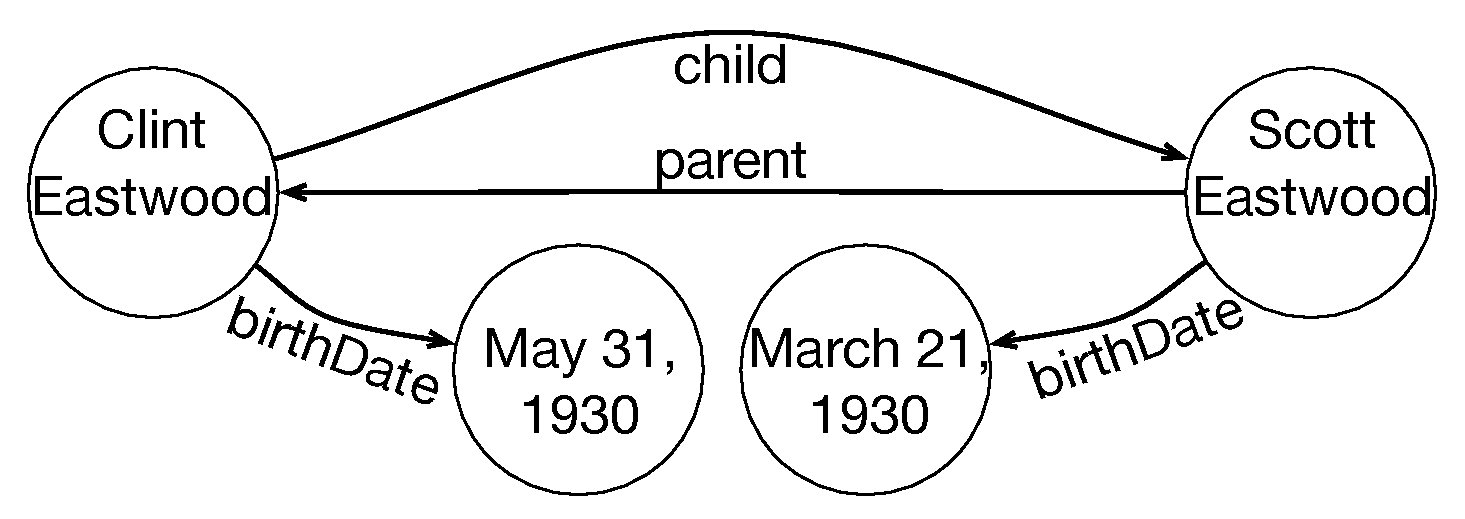
\includegraphics[width=0.8\columnwidth]{include/figure/graph_example.pdf}
	\vspace{-1ex}
	\caption{Graph example of \dbpedia for four triples.}
	\label{fig:krd_graph_example}
	\vspace{-3ex}
\end{figure}

%The data structure \krd leverages on is a straightforward translation of 
We translate a KB $\kb$ into a directed graph: entities and literals are the nodes, and there is a directed edge from node $a$ to node $b$ for each triple $\<a,rel,b\> \in \kb$. 
%IS THIS NOTATION NEW HERE???
Edges are labelled with the relation $rel$ that connects subject to object. Figure~\ref{fig:krd_graph_example} shows a portion of \dbpedia~\cite{bizer2009dbpedia} for four triples.
%that connects two person in child and parent relationships, along with their dates of birth. The graph represents information for four KB triples.
%(two birth dates, one parent, and one child relation).

The body of a rule can be seen as a path in the graph. In Figure~\ref{fig:krd_graph_example}, the body $\atom{child}{a}{b} \wedge \atom{parent}{b}{a}$ corresponds to the path \textit{Clint Eastwood} $\rightarrow$ \textit{Scott Eastwood} $\rightarrow$ \textit{Clint Eastwood}. 
As introduced in Section~\ref{sec:krd_language}, a valid body of a rule contains target variables $a$ and $b$ at least once, every other variable at least twice, and atoms are transitively connected. 
If we allow navigation of edges independently of the edge direction, we can translate bodies of valid rules to valid paths on the graph.
\begin{inparaenum}[(i)]
	Given a pair of entities $(x,y)$, a {\em valid body} corresponds to a valid path $p$ on the graph such that:
	\item $p$ starts at the node $x$;
	\item $p$ covers $y$ at least once;
	\item $p$ ends in $x$, in $y$, or in a different node that has been already visited.
\end{inparaenum}
%I DONT SEE CLEARLY THE TRANSLATION HERE, WHY IT HAS TO END in one of those? I would rather expect as third : p covers an incoming and out coming edge for each node different from x and y  %%%%%%%<<<<<<<<<<<<<<<
%NOT ESSENTIAL
%The transitive connection between atoms is always guaranteed by the construction property of a path $p$: for each node $n$ in $p$ there always exists a subpath that connects $n$ to every other node in $p$.
%
%In other words, 
Given the body of a rule $r_{body}$, $r_{body}$ covers a pair of entities $(x,y)$ iff there exists a valid path on the graph that corresponds to $r_{body}$. This implies that for a pair of entities $(x,y)$, we can generate bodies of all possible valid rules by computing all valid paths from $x$ to $y$ (and vice versa) with a standard BFS. The key point is the ability to navigate each edge in any direction by turning the original directed graph into an undirected one.
%is the VICE VERSA CORRECT?? <<<<
%Despite the navigation over an undirected graph
However, we need to keep track of the original direction of the edges. This is essential while translating paths to rule bodies. In fact, %if we navigate an edge \texttt{rel} between $a$ and $b$, going 
an edge directed from $a$ to $b$ produces the atom $\atom{rel}{a}{b}$, while $b$ to $a$ produces $\atom{rel}{b}{a}$. 
%The two atoms are different, as the facts exist in the KB only wrt the original direction of the edge (determined by the position of the variables).
%NOTICE A FEW CHANGES IN WORDING HERE

Since every node can be traversed multiple times, for two entities $x$ and $y$ there might exist infinite valid paths starting from $x$. This is avoided with a $maxPathLen$ parameter that constrains the search space by determining the maximum number of edges in the path. When translating paths to Horn Rules, $maxPathLen$ is the maximum number of atoms allowed in the body of the rule.
We will validate the use of this parameter in Section~\ref{sec:krd_experiments}. 
%This parameter is essential 
%to avoid the discovery of rules with infinite body length and 
%to constraint the search space.
We now describe the two main steps in our generation of the universe of all possible rules for $G$. 

\noindent \myparagraph{1. Create Paths}
%The main advantage of inspecting just the generation set $G$ is the capability of loading only a small portion of the graph that is currently needed. 
Given a pair of entities $(x,y)$, we retrieve from the KB all nodes at a distance smaller than $maxPathLen$ from $x$ or $y$, along with their edges. The retrieval is done recursively: we maintain a queue of entities, and for each entity in the queue we execute a SPARQL query against the KB to get all entities (and edges) at distance $1$ from the current entity -- we call these queries \emph{single hop queries}. At the $n$-th step, we add the new found entities to the queue iff they are at a distance less than $maxPathLen-n$ from $x$ or $y$ and they have not been visited before. The queue is initialized with $x$ and $y$. 
%By doing so we retrieve a small portion of the entire KB, the only one needed to discover rules that cover $(x,y)$. 
%We show in the experimental section that SPARQL engines are very fast at executing single hop queries. %DO WE REALLY SHOW IT?? <<<<
%
%\vspace{0.5ex}
%\myparagraph{Navigate Graph}
%The generation of the universe of all possible rules for $G$ is then straightforward: 
%For each element $(x,y) \in G$, we construct the 
Given the graph for every $(x,y)$, we then compute all valid paths starting from every $x$. 

\noindent \myparagraph{2. Evaluate Paths}
Computing paths for every example in $G$ implies also computing the coverage over $G$ for each rule. The {\em coverage} of a rule $r$ is the number of elements in $G$ for which there exists a path corresponding to $r_{body}$. 
%
%do we want to keep the following sentence ?? <<<<<<<<<<<<<<<<<<<<<<<< PAOLO REMOVED ACCORDING TO NEW SEC 3 $$$$$$$$$$$$$<<<<<<
%Our technique also generates single-instance rules: rules that cover only one example $(x,y) \in G$ by instantiating target variables $a$ and $b$ in the rule with $x$ and $y$. 
%
Once the universe of all possible rules has been generated (along with coverages over $G$), computing coverage and unbounded coverage over $V$ requires only the execution of two SPARQL queries against the KB for each rule in the universe (validation queries).
%REDUNDANT 
%We will show in Section~\ref{sec:krd_greedy} how some queries can be avoided, as well as there is no need of enumerating all possible rules in the universe as some of them will never be part of the final solution.

%Clearly, the size of $G$ has a direct impact on the search space and hence on the running time. Since we generate all valid rules for each example in $G$, the search space grows roughly linearly with the size of $G$. If we could know a-priori the minimum subset of examples that lead to the generation of all valid rules, then we could use only those few examples. 
%
%A future direction we are working on exploits exactly this point: how to select a small number of representative examples in order to reduce the size of $G$, without significantly affecting the quality of the output.
%\vspace{-1ex}

One of the goals is to discover more expressive rules. We therefore generate three new atom types as detailed next.

%\vspace{-1ex}
%\vspace{0.5ex}
\noindent \myparagraph{Literal comparison}
In Section~\ref{sec:krd_language} we defined our target language, which, other than predicate atoms, includes literal comparison. 
Their role is to enrich the language with comparisons among literal values other than equalities, such as ``greater than''. 
%or ``less than''. 
To discover such atoms, the graph representation must contain edges that connect literals with one (or more) symbol from $\{<,\leq,\neq,>,\geq\}$. As an example, Figure~\ref{fig:krd_graph_example} should contain an edge `$<$' from node ``\textit{March 31, 1930}'' to node ``\textit{March 21, 1986}". Unfortunately, the original KB does not contain this kind of information, and materializing such edges among all literals is infeasible.

%Once again, the use of a 
The generation set $G$ is the resource point to identify relevant literal comparison.
Since we discover paths for a pair of entities from $G$ in isolation, the size of a graph for a pair of entities is relatively small, thus we can afford to compare all literal values within a single example graph. 
%Since in a single example graph the number of literals is usually small, the creation of a quadratic number of edges w.r.t. the number of literals is affordable. 
%Despite this implies the creation of a quadratic number of edges w.r.t. the number of literals in the graph, within a single example graph the number of literals is usually small thus the quadratic comparison affordable. 
KBs include three types of literals: numbers, dates, and strings. Besides equality comparisons, we add `$>$',`$\geq$',`$<$',`$\leq$' relationships between numbers and dates, and $\neq$ between all literals. These new relationships are treated as normal atoms (edges): $x \geq y$ is equivalent to $\atom{rel}{x}{y}$, where \texttt{rel} is equal to $\geq$. 
%Once we added comparison edges for every input example graph, the discovery of literal comparisons is equivalent to discovering for predicate atoms.

\noindent \myparagraph{Not equal variables}
The ``not equal'' operator introduced for literals is useful for entities as well. 
Consider the rule:
$$ \atom{bornIn}{a}{x} \wedge x \neq b \Rightarrow \atom{notPresident}{a}{b} $$
It states that if a person $a$ is born in a country that is different from $b$, then $a$ cannot be the president of $b$.
%The rule holds for most of the countries in the world. 
One way to consider inequalities among entities is to add edges among all pairs of entities in the graph. However, this strategy is inefficient and would lead to many meaningless rules. To limit the search space while aiming at meaningful rules, we use the \texttt{rdf:type} triples associated to entities. We add an inequality edge in the input example graph only between those pairs of entities of the same type (as in the president example above). %, e.g., they belong to the same conceptual category. 
%As with the generation of $G$ and $V$, .  In the above rule it is reasonable to compare $x$ and $b$ because they are both countries.

\noindent \myparagraph{Constants}
Finally, we allow the discovery of rules with constant selections. % (entities). 
Suppose that for the above rule for president, all examples in $G$ are people born in the country ``\textit{U.S.A.}'', and there is at least one country for which this rule is not valid. According to our problem statement, the right rule is therefore:
%
$$ \atom{bornIn}{a}{x} \wedge x \neq \emph{U.S.A.} \Rightarrow \atom{notPresident}{a}{\emph{U.S.A.}} $$
%
To discover such atoms, %we introduce a refinement of the rule generation.
%For a given rule $r$, 
we promote a variable $v$ in a given rule $r$ to an entity $e$ iff for every $(x,y) \in G$ covered by $r$, $v$ can always be instantiated with the same value $e$. 
%In the example above, we promote variable $b$ to  ``\textit{U.S.A.}''.%}, generating the rule.

\vspace{-1ex}
\subsection{Input Example Generation} \label{sec:ex_generation}
\vspace{-1ex}
Given a KB $\kb$ and a predicate $rel \in \kb$, we automatically build a generation set $G$ and a validation set $V$ as follows. 
$G$ consists of positive examples for the target predicate $rel$, i.e., all pairs of entities $(x,y)$ such that $\<x,rel,y\> \in \kb$.
%, e.g., for target predicate is \texttt{child}, it consists of all pairs of entities in a child relation.
$V$ consists of counter (negative) examples for the target predicate.
These are more complicated to generate because of the open world assumption in KBs. 
Differently from classic databases, we cannot assume that what is not stated in a KB is false (closed world assumption), thus everything that is not stated is $unknown$. % rather than false. 
%This implies that 
However, since the likelihood of two randomly selected entities being a positive example is extremely low, one possible simple way of creating false facts is to randomly select pairs from the cartesian product of the entities~\cite{muggleton1994inductive}. While this process gives negative examples with a very high precision, only a very small fraction of these entity pairs are semantically related (something that is guaranteed for positive examples since pairs in $G$ are always connected at least by the target predicate). This semantic aspect has strong effects in the ultimate applications that use the generated negative examples. In fact, unrelated entities have less meaningful paths than semantically related entities and this is reflected in lower quality in the experimental results. 
%when we discover negative examples ($V$ is used as the generation set).
%We cannot take two entities that are not related by a property and assume that they form a negative example. 

To generate negative examples that are likely to be correct (true false facts) and that are semantically related in the KB, we mine the facts to identify the entities that are more likely to be complete (i.e., entities for which the KB contains every piece of information). This process is done exploiting and extending the popular notion of \emph{Local-Closed World Assumption} (\emph{LCWA})~\cite{dong2014data,galarraga2015fast}. 
%
LCWA states that if a KB contains one or more object values for a given subject and predicate, then it contains all possible values. For example, if a KB contains one or more children of Clint Eastwood, then it contains all his children. This is always true for \emph{functional} predicates (e.g., \texttt{capital}), 
% (predicates such as \texttt{capital} where the subject can have at most one object value), 
while it might not hold for non-functional ones (e.g., \texttt{child}). 
We extend this intuition also to predicates rather than entities. If a KB contains a relation between two entities $x$ and $y$, then it contains all relations between $x$ and $y$.

Now that we can identify entities that are likely to be complete, we generate negative examples taking the union of entities satisfying the LCWA: 
for a predicate $rel$, a negative example is a pair $(x,y)$ where either $x$ is the subject of one or more triples $\<x,rel,y'\>$ with $y \neq y'$, or $y$ is the object of one or more triples $\<x',rel,y\>$ with $x \neq x'$. 
For example, if $rel=\texttt{child}$, a negative example is a pair $(x,y)$ s.t. $x$ has some children in the KB who are not $y$, or $y$ is the child of someone who is not $x$. %By considering the union of the two LCWA aspects we do not restrict predicates to be functional (such as in~\cite{galarraga2015fast}). 
%not sure what is an aspect in the sentence above
Moreover, for a candidate negative example over entities $(x,y)$, $x$ must be connected to $y$ via a predicate that is different from the target predicate. In other words, given a KB $\kb$ and a target predicate $rel$, $(x,y)$ is a negative examples if $\<x,rel',y\> \in \kb$, with $rel' \neq rel$. 
These restrictions make the size of $V$ of the same order of magnitude of $G$ (see Section~\ref{sec:krd_experiments}), and guarantees that, for every $(x,y) \in V$, $x$ and $y$ are related by at least one predicate.



%% %%%%%%%%% COMMENTED BY PAOLO IN ICDE
%To mitigate this problem, and generate negative examples that are likely to be correct (true false facts), we are after entities that are more likely to be complete in their information. For this task, we %make use of a popular technique for KBs: 
%exploit the \emph{Local-Closed World Assumption} (\emph{LCWA})~\cite{dong2014data,galarraga2015fast}. LCWA states that if a KB contains one or more object values for a given subject and predicate, then it contains all possible values. For example, if a KB contains one or more children of Clint Eastwood, then it contains all his children. This is always true for \emph{functional} predicates (e.g., \texttt{capital}), 
%% (predicates such as \texttt{capital} where the subject can have at most one object value), 
%while it might not hold for non-functional ones (e.g., \texttt{child}). 
%%%%%%%%% COMMENTED BY PAOLO IN ICDE
%%KBs contain many non-functional predicates, we therefore extend the definition of LCWA by considering the dual aspect: if a KB contains one or more subject values for a given object and predicate, then it contains all values. 
%%NOT CLEAR WHY THE DUAL WILL HOLD, is this new? standard? why this depends on the large presence of "non-functional predicates"? <<<
%%check next sentence, rewritten heavily
%Given entities that are likely to be complete, we could generate negative examples taking the union of entities satisfying the LCWA: 
%for a predicate $rel$, a negative example is a pair $(x,y)$ where either $x$ is the subject of one or more triples $\<x,rel,y'\>$ with $y \neq y'$, or $y$ is the object of one or more triples $\<x',rel,y\>$ with $x \neq x'$. 
%For example, if $rel=\texttt{child}$, a negative example is a pair $(x,y)$ s.t. $x$ has some children in the KB who are not $y$, or $y$ is the child of someone who is not $x$. %By considering the union of the two LCWA aspects we do not restrict predicates to be functional (such as in~\cite{galarraga2015fast}). 
%%not sure what is an aspect in the sentence above
%
%The number of negative examples generated with the above technique is extremely large; for a target \texttt{child} predicate it is close to the cartesian product of all the people having a child with all the people having a parent. 
%% PROBLEM IN THE NEXT SENTENCE; I DON T BUY/UNDERSTAND THE JUSTIFICATION, WHY THEY NEED TO HAVE COMPARABLE SIZE? IS IT A REQUIREMENT OF THE ALGORITHM? IS IT RELATED TO THE WEIGHING SCHEME? WHAT HAPPENS IF THIS DOES NOT HAPPEN? <<<<<<<<<<<<<
%However, to apply the same approach for positive and negative rules discovery, we require $G$ and $V$ to be of comparable sizes. 
%%%%%%%%%%%%%%%%%%%%%%%%%%%%%%%%%%%%%%%%%%
%Instead of randomly selecting a subset, we introduce a further constraint that significantly reduces the size of $V$. 
%
%Given a candidate negative example over entities $(x,y)$, $x$ must be connected to $y$ via a predicate that is different from the target predicate. In other words, given a KB $\kb$ and a target predicate $rel$, $(x,y)$ is a negative examples if $\<x,rel',y\> \in \kb$, with $rel' \neq rel$. This intuition exploits the LCWA for predicates rather than for entities. If a KB contains a relation between two entities $x$ and $y$, then it contains all relations between $x$ and $y$.
%%. If $x$ and $y$ are in a relation that is not the target predicate, then 
%%and $x$ and $y$ are not connected by the target predicate. % in the real world. 
%This restriction makes the size of $V$ of the same order of magnitude of $G$ (see Section~\ref{sec:krd_experiments}), and guarantees the existence of a path between $x$ and $y$, for every $(x,y) \in V$. 
%%Since $V$ becomes the generation set in the negative rules discovery, $V$ should be small in size and it must guarantee the existence of a path between pairs of entities in each example. 
%Such a property is guaranteed in $G$, since pairs are always connected at least by the target predicate.
%%For positive examples, the existence of a path was already guaranteed since pairs in $G$ are always connected at least by the target predicate.
%
%Ultimately $V$ is generated by using both constraints. 
\begin{example}
	A negative example $(x,y)$ for the target predicate \texttt{child} has the following characteristics:
	\begin{inparaenum}[\itshape(i)]
		\item $x$ and $y$ are not connected by a \texttt{child} predicate;
		\item either $x$ has one or more children (different from $y$) or $y$ has one or more parents (different from $x$);
		\item $x$ and $y$ are connected by a predicate that is different from \texttt{child} (e.g., \texttt{colleague}).
	\end{inparaenum}
\end{example}

%STEFANO: WE CAN REMOVE THE NEXT IF WE DO NOT HAVE SPACE, NOT STRICTLY NECESSARY
%KBs use the same predicate to connect different types. For example, the \texttt{child} predicate is used to connect two entities of type person, but also two companies in an ownership relation. 
To enhance the quality of the input examples and avoid cases of mixed types, 
we require that for every example pair $(x,y)$ in either $G$ or $V$, $x$ and $y$ are always of the same \emph{type}. 
%ADDED BY STEFANO
Note that even when the LCWA does not hold, its negative impact is relatively low. In fact our negative examples are a subset of the cartesian product of all entities minus positive examples, and since the cartesian product contains very few positive examples (errors), also a subset of it will contain a limited amount of errors. We will validate this assumption in Section~\ref{sec:krd_int_evaluation}.
%we introduce the \emph{type} restriction when generating $G$ and $V$. The type restriction requires that for every example pair $(x,y)$ belonging to either $G$ or $V$, $x$ and $y$ are always of the same type across the pairs. 
%All KBs include entity types. % (often through the \texttt{rdf:type} statement), therefore we make use of this information. 
%For example, $G$ and $V$ for a target \texttt{child} predicate are two sets of pairs, where each pair consists in two entities of type person. The type information can be manually provided or, as we will see in Section~\ref{sec:krd_comparative}, we can automatically compute it from the KB.
%IS THE LAST SENTENCE NEEDED? can we just say that is there?



%NICE BUT MOVE TO RELATED
%To the best of our knowledge, \krd is the first approach that is capable of discovering both positive and negative rules in KBs. Previous works have put their focus either on the positive setting~\cite{abedjan2014amending,galarraga2015fast} (TODO: cite Ontological Pathfinding), or on the negative one (TODO: cite Data Lakes Sigmod). However, none of these techniques can be easily adapted to work in the dual scenario.

%\section{$A^*$ Greedy Algorithm} \label{sec:krd_greedy}
\section{Discovery Algorithm} \label{sec:krd_greedy}
We introduce a greedy approach to solve the approximate version of the discovery problem (Section~\ref{sec:krd_prob_def}). The algorithm combines two phases:
\begin{inparaenum}[\itshape(i)]
	\item it solves the set cover problem with a greedy strategy;
	\item it discovers new rules by navigating the graph in a $A^*$ search fashion.
	%, allowing the pruning of unpromising paths.	
\end{inparaenum}

\subsection{Marginal Weight}
%In Section~\ref{sec:krd_weight_fun}, we defined the weight associated with a set of rules $R$ with two components that model the role of positive and negative examples, respectively.
%as follows:
%\begin{equation*}
%w(R) = \alpha \cdot (1-\frac{\mid C_{R}(G)\mid}{\mid G \mid}) +\beta \cdot (\frac{\mid C_{R}(V) \mid}{\mid U_{R}(V)\mid})
%\end{equation*}
%Our goal is to discover a set of rules that covers as many elements as possible in $G$, and as few elements as possible in $V$. 
We follow the intuitions behind the greedy algorithm for weighted set cover by defining a \emph{marginal weight} for rules that are not yet included in the solution~\cite{chvatal1979greedy}.

\begin{definition}
	Given a set of rules $R$ and a rule $r$ such that $r \notin R$, the marginal weight of $r$ w.r.t. $R$ is defined as:
	\begin{equation*} \label{eq:mar_weight}
	w_m(r) = w(R \cup \{r\}) - w(R) 
	%- \alpha \cdot \frac{\mid C_{r}(G) \setminus C_{R}(G) \mid}{\mid G \mid} + \beta \cdot (\frac{\mid C_{R \cup \{r\}}(V) \mid}{\mid U_{R \cup \{r\}}(V) \mid} - \frac{\mid C_{R}(V) \mid}{\mid U_{R}(V) \mid})
		\vspace{-0.5ex}
	\end{equation*}
\end{definition}

The marginal weight quantifies the total weight increase of adding $r$ to an existing set of rules $R$. In other words, it indicates the contribution of $r$ to $R$ in terms of new elements covered in $G$ and new elements unbounded covered in $V$. Due to the first negative part of the weight, $w_m(r) \in [-\alpha,+\beta]$. Since the set cover problem aims at minimizing the total weight, we would never add a rule to the solution if its marginal weight is greater than or equal to $0$.

%%!TEX root = ../cleaning-vldb-16.tex
{\singlespacing
  \begin{algorithm}[t]\small
      \SetKwInOut{Input}{input}
      \SetKwInOut{Output}{output}
      
      \SetKwFunction{sinInRule}{singleInstanceRule}
      
	
      \SetKwData{mannot}{$\mathcal{M}_{annot}$}
	
      \Input{$G$ -- generation set}
      \Input{$V$ -- validation set}
      \Input{$R$ -- universe of rules}
      \Output{$R_{opt}$ -- greedy set cover solution}
      
      	$R_{opt} \gets \emptyset$\;
      	$r \gets \underset{w_m(r)}{\operatorname{argmin}}(r \in R)$\;
      	\Repeat{$R = \emptyset \vee C_{R_{opt}}(G) = G \vee w_m(r) \geq 0$}
      	{
      		$R_{opt} \gets R_{opt} \cup \{r\}$\;
      		$R \gets R \setminus \{r\}$\;
      		$r \gets \underset{w_m(r)}{\operatorname{argmin}}(r \in R)$\;
      	}
      	\If{$C_{R_{opt}}(G) \neq G$}{
      		$R_{opt} \gets R_{opt} \cup \sinInRule(G \setminus C_{R_{opt}}(G))$\;
      		
      	}
  
  \Return{$R_{opt}$}
  \caption{Greedy Rules Selection.}
  \label{alg:krd_greedy}
  \end{algorithm}
}

%Algorithm~\ref{alg:krd_greedy} shows the straightforward 
%In the greedy rule selection procedure. 
The algorithm for greedy rule selection is then straightforward:
given a generation set $G$, a validation set $V$, and the universe of all possible rules $R$, the algorithm picks at each iteration the rule $r$ with minimum marginal weight and add it to the solution $R_{opt}$.
%takes as input the generation set $G$, the validation set $V$, and the universe of all possible rules $R$. The set of output rules $R_{opt}$ is first assigned to an empty set. At each iteration, the algorithm picks from $R$ the rule $r$ with the minimum marginal weight, and it adds $r$ to $R_{opt}$, $r$ is then removed from $R$. 
The algorithm stops when one of the following termination conditions are met:
\begin{inparaenum} [\itshape1)]
	\item $R$ is empty -- all the rules have been included in the solution;
	\item $R_{opt}$ covers all elements of $G$;
	\item the minimum marginal weight is greater than or equal to $0$ -- among the remaining rules in $R$, none of them has a negative marginal weight.
	%, hence the current solution is the one with the minimum weight.
\end{inparaenum}
%WE CAN ELIMINATE THE NEXT SENTENCE IF WE NEED SPACE
If the second termination condition is not met, there may exist examples in $G$ that are not covered by $R_{opt}$. In such a case the algorithm will augment $R_{opt}$ with single-instance rules (rules that cover only one example), one for each element in $G$ not covered by $R_{opt}$.
%WILL? do we do it? <<<<<<<<

Since the coverage of a rule is always contained in its unbounded coverage, the marginal weight is greater than or equal to $0$ whenever the rule does not cover new elements in $G$ and does not unbounded cover new elements in $V$. 
%UNBOUND COVER? then below should be unbound covered, i guess <<<
%More specifically, a rule $r$ has a negative marginal weight iff the sum of its new elements covered in $G$ with its new elements unbounded covered in $V$ is strictly greater than its new elements covered in $V$ multiplied by some $\gamma$, where $\gamma$ depends on how we set $\alpha$ and $\beta$.

The greedy solution guarantees a \texttt{log($k$)} approximation
to the optimal solution~\cite{chvatal1979greedy}, where $k$ is the largest number of elements covered in $G$ by a rule in $R$ -- $k$ is at most $|G|$. If the output rules in the final solution cover disjoint sets of $G$, then the greedy solution coincides with the optimal one.

\subsection{$A^*$ Graph Traversal}
The greedy algorithm for weighted set cover assumes that the universe of rules $R$ has been generated.
%, so that we can iteratively pick the rule with minimum marginal weight. 
To generate $R$, we need to traverse all valid paths from a node $x$ to a node $y$, for every pair $(x,y) \in G$. But do we really need all possible paths for every example in $G$?
		\vspace{-1.5ex}

	\begin{figure}[htb]
		\centering
		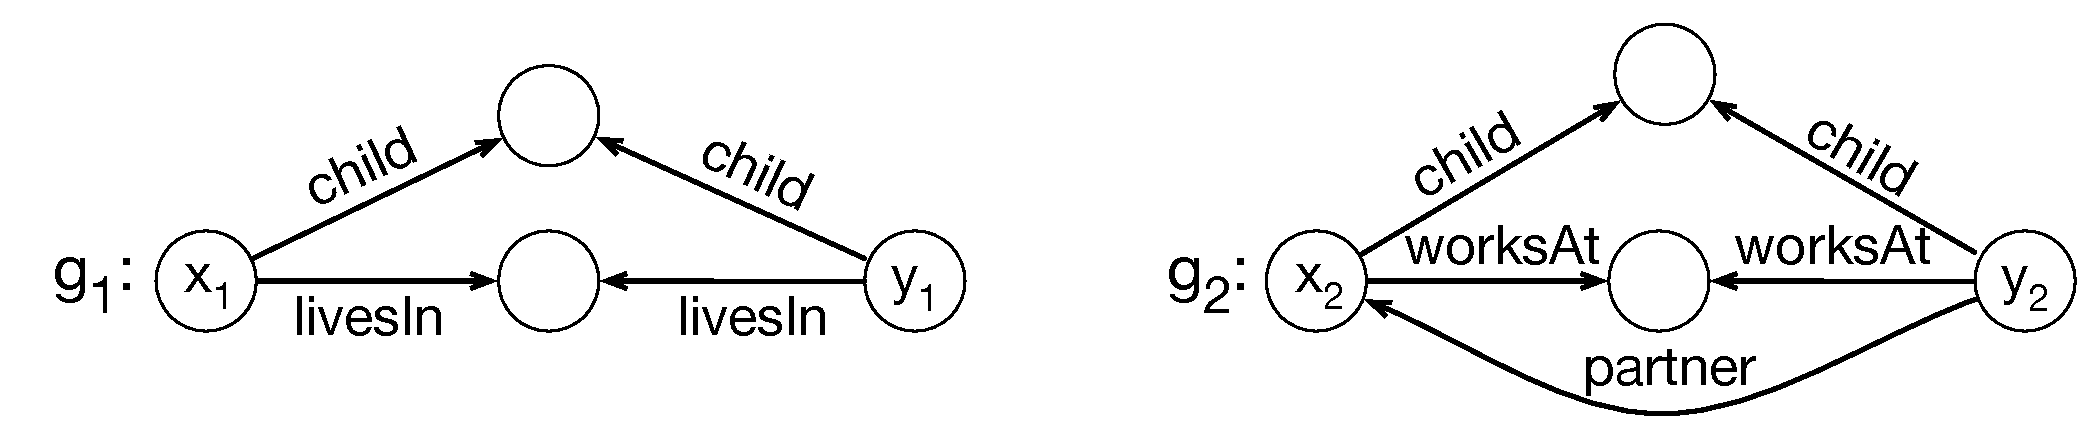
\includegraphics[width=0.99\columnwidth]{include/figure/a*_graph_example.pdf}	
		\vspace{-4ex}
		\caption{Two positive examples.}
	\label{fig:positive_examples}
\end{figure}
		\vspace{-1.5ex}

\begin{example}
	Consider the scenario where we are mining positive rules for the target predicate \texttt{spouse}. The generation set $G$ includes two examples $g_1$ and $g_2$, Figure~\ref{fig:positive_examples} shows the corresponding KB graphs. % for the two examples. 
	Assume for simplicity that all rules in the universe have the same coverage and unbounded coverage over the validation set $V$.
	One candidate rule is $r : \atom{child}{x}{v_0} \wedge \atom{child}{y}{v_0} \Rightarrow \atom{spouse}{x}{y}$, stating that entities $x$ and $y$ with a common child are married. Looking at the KB graph, $r$ covers both $g_1$ and $g_2$.
	%-- in both $g_1$ and $g_2$ there exists a path that corresponds to $r_{body}$. 
	Since all rules have the same coverage and unbounded coverage over $V$, 
	%if we include $r$ in the solution, %before inspecting other potential rules, then 
	there is no need to generate any other rule. In fact, any other candidate rule will not cover new elements in $G$, therefore their marginal weights will be greater than or equal to $0$. 
	%Hence any other rule will not be part of the solution. 
	Thus the creation and navigation of edges \texttt{livesIn} in $g_1$, \texttt{worksAt} in $g_2$, and \texttt{partner} in $g_2$ become worthless.
\end{example}

		\vspace{0.5ex}
Based on the above observation, we avoid the generation of the entire universe $R$, but rather consider at each iteration the most promising path on the graph. The same intuition  is behind 
the $A^*$ graph traversal algorithm~\cite{hart1968formal}. 
Given an input weighted graph, $A^*$ computes the smallest cost path from a starting node $s$ to an ending node $t$. At each iteration, $A^*$ maintains a queue of partial paths starting from $s$, and it expands one of these paths based on an \emph{estimation} of the cost to reach $t$. The path with the best estimation is expanded and added to the paths queue. The algorithm keeps iterating until one of the partial paths reaches $t$. 

We discover rules with a similar technique. For each example $(x,y) \in G$, we start the navigation from $x$. We keep a queue of not valid rules, % (Section~\ref{sec:krd_language}), 
and at each iteration we consider the rule with the minimum marginal weight, which corresponds to paths in the example graphs. 
We expand the rule by following the edges, and we add the new founded rules to the queue of not valid rules. Differently from $A^*$, we do not stop when a rule (path) reaches the node $y$. Whenever a rule becomes valid, we add the rule to the solution and we do not expand it any further. The algorithm keeps looking for plausible paths until one of the termination conditions of the greedy cover algorithm is met. %Algorithm~\ref{alg:krd_greedy} is met.

A crucial point in $A^*$ is the definition of the estimation cost. To guarantee the solution to be optimal, the estimation must be \emph{admissible}, i.e., the estimated cost must be less than or equal to the actual cost. 
For example, for the shortest route problem, an admissible estimation is the straight-line distance to the goal for every node, as it is physically the smallest distance between any two points. In our setting, given a rule that is not yet valid and needs to be expanded, we define an admissible estimation of the marginal weight.

\begin{definition}
	Given a rule $r : A_1 \wedge A_2 \cdots A_n \Rightarrow B$, we say that a rule $r'$ is an \emph{expansion} of $r$ iff $r'$ has the form $A_1 \wedge A_2 \cdots A_n \wedge A_{n+1} \Rightarrow B$. %In other words, $r'$ is generated by adding a new atom to the body of $r$.
\end{definition}
%WE ALREADY USED expand MULTIPLE TIMES ABOVE. Should this go earlier? is it needed? <<<<

In other words, expanding $r$ means adding a new atom to the body of $r$. In the graph traversal, expanding $r$ means traversing one further edge on the path defined by $r_{body}$. To guarantee the optimality condition, the estimated marginal weight for a rule $r$ that is not valid must be less than or equal to the actual weight of any valid rule that is generated by expanding $r$. Given a rule and some expansions of it, we can derive the following.

\begin{lemma} \label{lemma:krd_exp_cov}
	Given a rule $r$ and a set of pair of entities $E$, then for each $r'$ expansion of $r$, $C_{r'}(E) \subseteq C_r(E)$ and $U_{r'}(E) \subseteq U_r(E)$.
\end{lemma}
\vspace{0.5ex}

The above Lemma states that the coverage and unbounded coverage of an expansion $r'$ of $r$ are contained in the coverage and unbound coverage of $r$, respectively, and directly derives from the augmentation inference rule for functional dependencies~\cite{abiteboul1995foundations}. 
%In fact, expanding a rule with a new atom to its body makes the rule more selective. 
%This is equivalent of adding an `AND' condition to a SQL query $q$: the new result will obviously be a subset of the result obtained with $q$.
%Note that Lemma~\ref{lemma:krd_exp_cov} is equivalent to the 

%We recall that the merginal weight of a rule $r$ w.r.t. a solution $R$ is defined as follow:
%\begin{equation*}
%w_m(r) = - \alpha \cdot \frac{\mid C_{r}(G) \setminus C_{R}(G) \mid}{\mid G \mid} + \beta \cdot (\frac{\mid C_{R \cup \{r\}}(V) \mid}{\mid U_{R \cup \{r\}}(V) \mid} - \frac{\mid C_{R}(V) \mid}{\mid U_{R}(V) \mid})
%\end{equation*}
The only positive contribution to marginal weights is given by $|C_{R \cup \{r\}}(V)|$. $|C_{R \cup \{r\}}(V)|$ is equivalent to $|C_{R}(V)| + |C_r(V) \setminus C_R(V)|$, thus if we set $|C_r(V) \setminus C_R(V)|=0$ for any $r$ that is not valid, we guarantee an admissible estimation of the marginal weight. We therefore estimate the coverage over the validation set to be $0$ for any rule that can be further expanded, since expanding the rule may bring its coverage to $0$.
%CANNOT NOT NOTICE HOW BRUTAL IT"S THIS ESTIMATE!

\begin{definition}\label{def:est_res_wei}
	Given a \emph{not valid} rule $r$ and a set of rules $R$, we define the \emph{estimated marginal weight} of $r$ as:
	\begin{equation*}
	w_m^*(r) = - \alpha \cdot \frac{\mid C_{r}(G) \setminus C_{R}(G) \mid}{\mid G \mid} + \beta \cdot (\frac{\mid C_R(V) \mid}{\mid U_{R \cup \{r\}}(V) \mid} - \frac{\mid C_{R}(V) \mid}{\mid U_{R}(V) \mid})
	\end{equation*}
	%where a rule is valid iff it respects the language biases defined in Section~\ref{sec:krd_language}.
\end{definition}
%I AM A BIT CONFUSED BY THE FORMULA, i was expecting a 0 in the first case <<<<<

The estimated marginal weight for a valid rule instead is equal to the actual marginal weight defined in Equation~\ref{eq:mar_weight}. Valid rules are not considered for expansion, therefore we do not need to estimate their weights since we know the actual ones. Given Lemma~\ref{lemma:krd_exp_cov}, we can easily see that $w_m^*(r) \leq w_m^*(r')$, for any $r'$ expansion of $r$. Thus our marginal weight estimation is admissible.

We use the concept of \emph{frontier nodes} for a rule $r$ ($N_f(r)$). Given a rule $r$, $N_f(r)$ contains the last visited nodes in the paths that correspond to $r_{body}$ from every example graphs covered by $r$. As an example, given $r_{body} = \atom{child}{x}{v_0}$, $N_f(r)$ contains all the entities $v_0$ that are children of $x$, for every $(x,y) \in G$. 
%-- $v_0$ is the last visited node in the path. 
Expanding a rule $r$ implies navigating a single edge from any frontier node. Algorithm~\ref{alg:krd_a*} shows the modified set cover version that includes $A^*$-like rules generation. The set of frontier nodes is initialized with starting nodes $x$, for every $(x,y) \in G$ (Line~\ref{alg_line:front_nodes}). The algorithm maintains a queue of rules $Q_r$, from which it chooses at each iteration the rule with minimum approximated weight. 
%approximated?? <<
The function \texttt{expandFrontiers} retrieves from the KB all nodes (along with edges) at distance $1$ from frontier nodes and returns the set of all rules generated by this one hop expansion. Such expansions are computed with efficient single-hop SPARQL queries. $Q_r$ is therefore initialized with all rules of length $1$ starting at $x$ (Line~\ref{alg_line:sparql_1}). In the main loop, the algorithm checks if the current best rule $r$ is valid or not. If $r$ is valid, $r$ is added to the output and it is not expanded (Line~\ref{alg_line:valid_rule}). If $r$ is not valid, $r$ is expanded iff the length of its body is less than $maxPathLen$ (Line~\ref{alg_line:exp_condition}). 
%Rules with body greater than or equal to $maxPathLen$ are not expanded as they are not allowed in the output. 
The termination conditions and the last part of the algorithm are the same of the previously described greedy set-cover algorithm. % Algorithm~\ref{alg:krd_greedy}.

%to remove vertical space after algorithm
\setlength{\textfloatsep}{0pt}% Remove \textfloatsep
{\singlespacing
  \begin{algorithm}[t]\small
      \SetKwInOut{Input}{input}
      \SetKwInOut{Output}{output}
      
      \SetKwFunction{expFron}{expandFrontiers}
      \SetKwFunction{frontiers}{frontiers}
      \SetKwFunction{isValid}{isValid}
      \SetKwFunction{length}{length}
      \SetKwFunction{sinInRule}{singleInstanceRule}
      
	
      \SetKwData{mannot}{$\mathcal{M}_{annot}$}
	
      \Input{$G$ -- generation set}
      \Input{$V$ -- validation set}
      \Input{$maxPathLen$ -- maximum rule body length}
      \Output{$R_{opt}$ -- greedy set cover solution}
      
      	$R_{opt} \gets \emptyset$\;
      	$N_f \gets \{x | (x,y) \in G\}$\; \label{alg_line:front_nodes}
      	$Q_r \gets \expFron(N_f)$\; \label{alg_line:sparql_1}
      	%$\quad$\tcp{SPARQL}%
      	$r \gets \underset{w_m^*(r)}{\operatorname{argmin}}(r \in Q_r)$\; \label{alg_line:q_r_initialisation}
      	\Repeat{$Q_r = \emptyset \vee C_{R_{opt}}(G) = G \vee w_m^*(r) \geq 0$}
      	{
      		$Q_r \gets Q_r \setminus \{r\}$\;
      		\If{$\isValid(r)$}{
      			$R_{opt} \gets R_{opt} \cup \{r\}$\; \label{alg_line:valid_rule}
      		}
      		\Else{
      			\tcp{rules expansion}
      			\If{$\length(r_{body}) < maxPathLen$ \label{alg_line:exp_condition}}
      			{
      				$N_f \gets \frontiers(r)$\;
      				$Q_r \gets Q_r \cup \expFron(N_f)$\;  \label{alg_line:sparql_2}
	      			%$\quad$\tcp{SPARQL}
      			}
      		}
      		$r \gets \underset{w_m^*(r)}{\operatorname{argmin}}(r \in Q_r)$\;
      	}
      	\If{$C_{R_{opt}}(G) \neq G$}{
      		$R_{opt} \gets R_{opt} \cup \sinInRule(G \setminus C_{R_{opt}}(G))$\;
      		
      	}
  
  \Return{$R_{opt}$}
  \caption{\krd Rule Discovery.}
  \label{alg:krd_a*}
  \end{algorithm}
}
\vspace{-2ex}
%restablish some space
\setlength{\textfloatsep}{5pt}

The simultaneous rules generation and selection of Algorithm~\ref{alg:krd_a*} brings multiple benefits. First, we do not generate the entire graph for every example in $G$. Nodes and edges are generated \emph{on demand}, whenever the algorithm requires their navigation (Line~\ref{alg_line:sparql_2}). If the initial part of a path is not promising according to its estimated weight, the rest of the path will never be materialized. % since there is no need to navigate it. 
%Materializing the graph is an expensive task, since we need to query the disk to retrieve target nodes and edges. 
Rather than materializing the entire graph and then traversing it, our solution gradually materializes parts of the graph whenever they are needed for navigation (Lines~\ref{alg_line:sparql_1} and~\ref{alg_line:sparql_2}). 
Second, the weight estimation leads to pruning unpromising rules. If a rule does not cover new elements in $G$ and does not unbounded cover new elements in $V$, then its estimated marginal weight is $0$ and will be pruned away. 
%A rule with $0$ marginal weight is never picked for expansion.
%A BIT PUZZLED, we have tons of rules with estimated marginal weight, no? <<<<<<<<
%, and if it is the algorithm terminates (due to one of the termination conditions). This implies that a rule with $0$ estimated marginal weight is pruned away from the search space, as we will never generate rules from its expansion.

%FOLLOWING PARAGRAPH REMOVED for the sake of SPACE. TO BE RECYCLED somewhere else?? <<<<<
%The partial materialization of the graph and the pruning of the search space have a significant impact on the algorithm's resources. The running time is halved in the worst case and ten times faster in the best one. We also significantly decrease the amount of memory needed, since we load sub-portions of the graph. Consider the extreme case where there exists a rule $r$ that covers all elements in $G$, unbound covers all elements in $V$ and does not cover any element of $V$. In such a case, Algorithm~\ref{alg:krd_a*} will output the optimal solution by just materialising paths on the example graphs that correspond to $r_{body}$ with $\bigO{l \cdot |G|}$ SPARQL queries, where $l$ is the length of $r_{body}$.







\section{Experiments} \label{sec:krd_experiments}
We implemented the above techniques in \krd, our system for \underline{Ru}le \underline{Di}scovery in \underline{K}nowledge Bases.
We carried out an extensive experimental evaluation of our approach and grouped the results in four main sub-categories: 
\begin{inparaenum}[\itshape(i)]
	\item demonstrating the quality of our output for positive and negative rules;
	\item comparing our method with the state-of-the-art systems;
	\item showing the applicability of rule discovery in Machine Learning algorithms with representative training data;
	\item testing the role of the parameters in the system. % settings and some KB properties.
\end{inparaenum}
%DO WE EVALUATE SAMPLING ON A DIFFERENT SECTION?

\myparagraph{Settings}
%We evaluated our approach over several popular KBs. 
%For each KB, 
%We downloaded the most up-to-date core facts and loaded them into our SPARQL query engine. We experimented with several SPARQL engines, 
%not relevant discussing sparql engines
%including \system{Jena ARQ}\footnote{\url{https://jena.apache.org/documentation/query/}}, \system{OWLIM %Lite}\footnote{\url{https://confluence.ontotext.com/display/OWLIMv54/OWLIM-Lite+Installation}}, and %\system{RDF-3x}\footnote{\url{https://code.google.com/archive/p/rdf3x/}}. We also implemented a na\"ive %relational database solution with \system{PostgreSQL}. 
%and eventually we opted for \system{OpenLink Virtuoso},
%\footnote{\url{http://virtuoso.openlinksw.com/}}
%as it was the fastest among all the solutions. 
%\system{Virtuoso} took on average 20 minutes to load a medium size KB (i.e., 10 GB) into its store, and %around 100 milliseconds to execute a single hop query. 
We ran experiments over the latest core facts derived from several KBs. All experiments were run on a desktop with a quad-core i5 CPU at 2.80GHz and 16GB RAM. We used \system{OpenLink Virtuoso}, optimized for 8GB RAM, with its SPARQL query endpoint on the same machine.

%In the following, 
Parameters $\alpha$ and $\beta$ of Equation~\ref{eq:weight_fun} were set to  $\alpha=0.3$ and $\beta=0.7$ for positive rules, and to $\alpha=0.4$ and $\beta=0.6$ for negative rules. 
%We also use a $maxPathLen$ parameter indicating the maximum number of atoms in each of the rules to be discovered that is set to $3$. 
We set the maximum number of atoms 
admissible in the body of a rule ($maxPathLen$) to $3$.
We analyze the role of these parameters in Section~\ref{sec:krd_int_evaluation}. 
\begin{comment}
Our method needs the two input parameters $\alpha$ and $\beta$ of Equation~\ref{eq:weight_fun}. 
We set $\alpha=0.3$ and $\beta=0.7$ for positive rules, while $\alpha=0.4$ and $\beta=0.6$ for negative rules. We empirically justify this choice in Section~\ref{sec:krd_int_evaluation}.
%$\alpha$ measures the importance of the coverage over the generation set, while $\beta$ measures the coverage over the validation set. In other words, a high $\alpha$ privileges recall over precision, while a high $\beta$ gives more importance to precision. We can afford a high $\alpha$ and a low $\beta$ when the input KB is accurate and complete. We will show that KBs contain many errors and missing information, therefore we set $\alpha = 0.3$ and $\beta = 0.7$. Increasing $\alpha$ and decreasing $\beta$ means a higher number of output rules with a lower accuracy. 
We also set the $maxPathLen$ parameter to $3$. This number represents the maximum number of atoms that we can have in the body of a rule. We will outline in Section~\ref{sec:krd_int_evaluation} that increasing this parameter does not bring any benefits, as rules with a body longer than $3$ atoms start to be very complicated and not insightful.
\end{comment}

\myparagraph{Evaluation Metrics}
We evaluated the effectiveness of \krd in discovering both positive and negative rules. The set of predicates for evaluation were chosen separately in the case of positive and negative rules from each KB.
For every KB, we first ordered predicates according to descending popularity (i.e., number of triples having that predicate). We then picked the top $3$ predicates for which we knew there existed at least one meaningful rule, and other $2$ top predicates for which we did not know whether some meaningful rules existed or not. 
%: we picked $5$ popular predicates occurring in a majority of triples out of which the top $3$ are known to have at least one meaningful rule, while there is no prior knowledge about the rules for the next 2 predicates. 

The evaluation of the discovered rules 
%discovered by \krd and the baseline algorithms we compare against 
%was done for both positive and negative rules 
has been done according to the state of the art for rule quality evaluation~\cite{galarraga2015fast}. If a rule was clearly semantically correct, we marked all its results over triples as true. If a rule correctness was unknown, we randomly sampled 30 triples either among the new facts (for positive rules) or among the errors (for negative rules), 
%new predictions likely to be violating rule head 
and manually checked them. % against the Web. 
The \emph{precision} of a rule is then computed as the ratio of correct assertions out of all assertions. 
%The subtle difference is that the sample set of tentatively violating predictions to be evaluated are generated differently for positive and negative rules. As an example, for the positive rule $\atom{spouse}{a}{v0} \wedge \atom{child}{v0}{b} \Rightarrow \atom{child}{a}{b}$, we retrieve all those pairs  $(a,b)$ such that $b$ is the child of $v0$ and $v0$ is the spouse of $a$ but $b$ is not the child of $a$. In the case of the negative rule, $\atom{child}{a}{b} \Rightarrow \neg \atom{spouse}{a}{b}$, we retrieve all those pairs $(a,b)$ such that $b$ is \texttt{child} of $a$ and $a$ is \texttt{spouse} with $b$.
\begin{comment}
\krd discovers rules for a given target predicate. For each KB, we chose $5$ representative predicates as follows: we first ordered predicates according to descending popularity (i.e., number of triples having that predicate), and then we picked the top $3$ predicates for which we knew there existed at least one meaningful rule, and other $2$ top predicates for which we did not know whether some meaningful rules existed or not. We repeated the procedure for each input KB, and for both positive and negative rules. Despite working with one predicate at a time, \krd can also discover rules for the entire KB by enumerating all the predicates in the KB, and discovering rules for each of them. We will show in Section~\ref{sec:krd_comparative} how this can be achieved.

Positive rules are very useful to enrich the KB by discovering new facts. 
%Since we are generating new data, we cannot evaluate the output over the existing data. 
Inspired by~\cite{galarraga2015fast}, we proceed as follows: we run the algorithm over the KB, and for each output rule we generate all new predictions that are not already in the KB (we execute the body of the rule against the KB and remove all those pairs that are already connected by the target predicate in the KB). 
%As an example, for the rule $\atom{spouse}{b}{a} \Rightarrow \atom{spouse}{a}{b}$, we retrieve all pairs %$(b,a)$ such that $b$ is \texttt{spouse} with $a$ but $a$ is not \texttt{spouse} with $b$ in the KB. 
If a rule is universally correct 
%(like the previous example)
, we mark all its new predictions as true. If a rule is unknown, we randomly sampled 30 new predictions and manually checked them against the Web. The \emph{precision} of a rule is then computed as the ratio of true predictions out of true and false predictions.

Negative rules are slightly more complicated to evaluate. In fact, despite KBs being usually incomplete, a large percentage of the data not stated in a KB is false. 
%-- a very small fraction of the cartesian product of all the people in a KB will be actually married.
Therefore negative rules will always discover many correct negative facts. However, negative rules are a great means to discover errors in the KB, and we leverage this aspect to evaluate them. For each discovered rule, we retrieve from the KB the pairs of entities for which the body of the rule can be instantiated over the KB and that are also connected by the target predicate. As an example, for the rule $\atom{child}{a}{b} \Rightarrow \neg \atom{spouse}{a}{b}$, we retrieve all those pairs $(a,b)$ such that $b$ is \texttt{child} of $a$ and $a$ is \texttt{spouse} with $b$. We call these generated pairs of entities \emph{potential errors}. Similar to positive rules, whenever a rule is universally correct we mark all its potential errors as true, whereas if the rule is unknown we manually check 30 sampled potential errors. The final precision of a rule is computed as actual errors divided by potential errors.


%The following can be skipped
%Furthermore, a potential error is evaluated as actual error whenever a single atom in the rule is incorrect, no matter if the atom is in the body or the head of the rule. For the negative rule $\atom{child}{a}{b} \Rightarrow \neg \atom{spouse}{a}{b}$, a specific instantiation $(a,b)$ is an actual error if either $b$ is not an actual \texttt{child} of $a$, or $b$ is not an actual \texttt{spouse} of $a$. As we will explain further below, negative rules cannot point exactly where the error is, but they give a hint that something is wrong and needs to be further inspected.
\end{comment}

Full test results, including KBs, induced rules, annotated examples and rules are available at \url{http://bit.ly/2csROsc}.


%\vspace{-1ex}
{\small
\begin{table}[thb]
	\centering
	\caption{Dataset characteristics.}
	\label{tab:krdDatasetDescr}
	\begin{small}
		\begin{tabular}
			{|>{\centering}m{1.2cm}|>{\centering}m{1.1cm}|>{\centering}m{1.15cm}|c|>{\centering}m{1.5cm}|}
			\hline
			\hline
			{\it KB}&{\it Version}&{\it Size}&{\it  \#Triples}&{\it \#Predicates} \tabularnewline
			\hline
			\dbpedia & 3.7 & 10.056GB & 68,364,605 & 1,424 \tabularnewline
			\yago & 3.0.2 & 7.82GB & 88,360,244 & 74 \tabularnewline
			\wikidata & 20160229 & 12.32GB & 272,129,814 & 4,108 \tabularnewline
			\hline
		\end{tabular}
	\end{small}
\end{table}
}

\vspace{-1ex}
\subsection{Quality of Rule Discovery in \krd} \label{sec:gen_evaluation}
\vspace{-1ex}
The first set of experiments aimed at evaluating the accuracy of discovered rules over three popular KBs: \dbpedia~\cite{bizer2009dbpedia}, \yago~\cite{suchanek2007yago}, and \wikidata~\cite{vrandevcic2014wikidata}. 
%For each KB we downloaded the most recent version and selected core facts, facts about people, geolocations and transitive \texttt{rdf:type} facts. \wikidata provides the entire dump alone; therefore we just eliminated from it all the non-English literal values. 
Table~\ref{tab:krdDatasetDescr} shows the characteristics of the KBs.

%As the figure shows, 
The size of the KB is important as loading the entire KB in memory is not feasible unless we either have HW with large amount of memory~\cite{Chen:2016,DBLP:conf/sigmod/FaridRIHC16}, or we shrink the KB by eliminating all the literals~\cite{galarraga2015fast}. In our approach, only a small portion of the KB is loaded in memory, thus we can afford to (i) discover rules with commodity HW resources, (ii) retain the literals, which are crucial for the value comparison in our rules. While \krd mines rules for a given target predicate at a time, it discovers rules over the entire KB given its set of predicates. This is further elaborated in Section~\ref{sec:krd_comparative}.

\begin{table}[ht]
%\vspace{-2ex}
	\centering
	\caption{\krd Positive Rule Accuracy.}
	\label{tab:pos_rules_acc}
	\begin{small}
	\begin{tabular}{|c|c|c|c|c|}
		\hline
		\hline
		{\it KB}&{\it Avg. Run Time}&{\it Avg. Precision}&{\it \# Annotations} \tabularnewline
		\hline
		\dbpedia & 34min, 56sec & \textbf{63.99}\% & 139\tabularnewline
		\yago &  59min, 25sec & \textbf{62.86}\% & 150\tabularnewline
		\wikidata &  2h, 21min, 34sec & \textbf{73.33}\% & 180\tabularnewline
		\hline
	\end{tabular}
	\end{small}
\end{table}
\vspace{-1ex}


\myparagraph{Positive Rules \krd} 
We first evaluate the precision for the positive rules on the top 5 predicates for each KBs. 
The number of new induced facts varies significantly from rule to rule.
% -- a rule with literals comparison produces a very high number of facts. In order 
To avoid the overall precision to be dominated by such rules, we first compute the precision for each rule as explained above, and then average values over all induced rules.
 Table~\ref{tab:pos_rules_acc} reports precision values, along with predicates average running time.
 Column \emph{\# Annotations}  reports the size of the sample of manually annotated triples.



Results show that the more accurate is the KB, the better is the quality of the induced rules. \wikidata contains very few errors, since it is manually curated, while
%and every triple is manually checked by different individuals before being inserted
 \dbpedia and \yago are automatically generated by extracting information from the Web, hence their quality is significantly lower. 
\begin{comment}
Discovering perfect positive rules is a hard task, mostly because there is no guarantee of the existence of valid negative examples. A striking example in this direction is one of the rule induced for \texttt{founder} in \dbpedia. Our approach discovers that if a person is born in the same place where a company is founded, then the person is the founder. The rule is obviously wrong
%, as there are many people who are born in the same place of a company and have not founded the company
. However this rule has a very high coverage over the generation set (many companies' founders founded their company in their birth place), and a very low coverage over the validation set -- among the cartesian product of all the people and companies, a very small fraction includes people and companies born and founded in the same place. Despite such hard cases, our approach is always capable of producing correct rules for those predicates for which we knew there existed some valid rules. 
\end{comment}
Some predicates, such as \texttt{academicAdvisor}, \texttt{child}, and \texttt{spouse}, have a precision above $95\%$ in all KBs, but average precision values are brought down by few predicates, such as \texttt{founder}, where meaningful positive rules probably do not exist at all. In other terms, when a rule exists, the system was able to find, but it was not able to recognize cases where no positive rules exist (indeed it is not possible to derive a founder from the information on persons and company in the KBs). 

The running time is influenced by the size of the KB with the number of triples and the number of predicates. %\krd is slower in \wikidata, which is the biggest KB.
 The more predicates we have in the KB, the more alternative paths we test while traversing the graph.
% thus resulting in a bigger search space. 
Another relevant aspect is the target predicate involved. Some entities have a huge number of outgoing and incoming edges, entity ``\textit{United States}'' in \wikidata has more than $600$K. When the generation set includes such entities, the navigation of the graph is slower as we traverse a large number of edges. 
%This is what happens in \yago, where the most popular predicates are \texttt{isLeaderOf} and \texttt{exports}. 
Parameter $maxPathLen$  also impacts the running time. The longer the rule, the bigger is the search space, as we discuss in Section~\ref{sec:krd_int_evaluation}. 
%We will show in the next Section how we can be much faster if we set to 2 atoms the maximum length of the rule. In the next chapter we will discuss some future directions to significantly cut down the running time based on the above observations.


%\vspace{1ex}
\begin{table}[htb]
	\centering
	\caption{\krd Negative Rule Accuracy.}
	\label{tab:neg_rules_acc}
	\begin{small}
	\begin{tabular}{|c|c|c|c|}
		\hline
		\hline
		{\it KB}&{\it Avg. Run Time}&{\it \# Pot. Errors} & {\it Precision} \tabularnewline
		\hline
		\dbpedia & 19min, 40sec& 499 (84) & \textbf{92.38}\%\tabularnewline
		\yago & 10min, 40sec & 2,237 (90) & \textbf{90.61}\%\tabularnewline
		\wikidata & 1h, 5min, 38sec & 1,776 (105)& \textbf{73.99}\%\tabularnewline
		\hline
	\end{tabular}
	\end{small}
\end{table}

\myparagraph{Negative Rules \krd} 
%Negative rules are very useful to discover inconsistencies in the KB. 
We evaluated negative rules as the percentage of correct errors discovered for the top 5 predicates in each KB. Table~\ref{tab:neg_rules_acc} shows, for each KB, the total number of potential erroneous triples discovered with the rules, whereas the precision is computed as the percentage of actual errors among potential errors. Numbers in brackets show the sample of unknown triples manually annotated.

Negative rules have better accuracy than positive ones. 
This is due to the fact that negative rules exist more often then positive rules.
% completeness of the validation set: for negative rules the validation set is the universe of all possible counter examples stated in the KB, whereas for positive rules the validation set is a small fraction of it. %Therefore negative rules are usually better validated than positive ones. 
%As expected, for the manually curated \wikidata, the precision of the rules is higher, and the absolute number of errors identified is lower because it does not contain as many errors as \dbpedia and \yago.
%For example, we identify the same rule that two people with same gender cannot be married both in \yago and \wikidata. Such a rule has a 94\% precision in \yago, while the accuracy in \wikidata is 57\%.
 \yago has the highest number of errors; for example, there are $9,057$ cases in the online \yago where a child is born before the parent. 
%We cannot point exactly where the error is -- there could be an error in one of the birth dates or an error in the parent relation -- but we can affirm that at least one of these values is wrong and send them to human evaluators to spot the inconsistency.
%
Differently from positive rules, literals play a key role in negative rules. In fact, several correct negative rules rely on temporal aspects in which something cannot happen before/after something else. Temporal information are usually expressed through dates, years, or other primitive types that are represented as literal values in KBs.

Discovering negative rules is faster than discovering positive rules
%.This is due to the time spent executing 
because of the different nature of the examples covered by validation queries. 
Whenever we identify a candidate rule, we execute the body of the rule against the KB with a SPARQL query to compute its coverage over the validation set. 
These queries are faster for negative rules since the validation set is simply all the entities directly connected by the target predicate, whereas in the positive case the validation set corresponds to counter examples that do not have this property and are more expensive to evaluate for SPARQL engines.
%, as discussed in Section~\ref{sec:ex_generation}.

%DO NOT SHOW RULES EXAMPLES
%Table~\ref{tab:neg_rules_acc} shows some interesting cases, for both correct and incorrect rules.
%The example rules show the full power of our language, including literals, smart literals comparisons, entities inequalities and constants. As previously mentioned, the extension including literals comparisons and entities inequalities gives a significant boost in accuracy for negative rules, while it is rarely used in discovery positive rules. The full set of discovered rules can be inspected online (TODO: footnote online appendix).
%
%\begin{table}[htb]
%	\centering
%	\label{tab:krd_rules_example}
%	\begin{small}
%		\begin{tabular}{>{\centering}m{10cm}|c|c}
%			{\it Rule}&{\it KB}&{\it Precision} \tabularnewline
%			\hline
%			$\atom{notableWork}{b}{a} \Rightarrow \atom{creator}{a}{b}$ & \wikidata & \textbf{100}\% \tabularnewline
%			$\atom{nationality}{a}{v_0} \wedge \atom{nationality}{b}{v_0} \wedge \atom{notableStudent}{b}{a} \Rightarrow \atom{academicAdvisor}{a}{b} $ & \dbpedia & \textbf{100}\% \tabularnewline
%			$\atom{hasChild}{v_0}{b} \wedge \atom{isMarriedTo}{a}{v_0} \Rightarrow \atom{hasChild}{a}{b}$ & \yago & 50\% \tabularnewline
%			$\atom{activeYearsEndDate}{a}{v_0} \wedge \atom{activeYearsStartDate}{b}{v_0} \Rightarrow \atom{successor}{a}{b}$ & \dbpedia & 0\% 
%			\tabularnewline 
%			$\atom{inception}{a}{v_0} \wedge \atom{dateOfBirth}{b}{v_1} \wedge v_1 > v_0 \Rightarrow \neg \atom{founder}{a}{b} $  & \wikidata & \textbf{100}\% 
%			\tabularnewline 
%			$\atom{country}{a}{England} \wedge \atom{country}{b}{United\_Kingdom} \wedge England \neq United\_Kingdom \Rightarrow \neg \atom{county}{a}{b}$ & \dbpedia & \textbf{100}\% \tabularnewline
%			$\atom{actedIn}{a}{b} \Rightarrow \neg \atom{wroteMusicFor}{a}{b}$ & \yago & 40\% \tabularnewline
%			$\atom{birthYear}{a}{v_0} \wedge \atom{birthDate}{b}{v_1} \wedge v_0 < v_1 \Rightarrow \neg \atom{academicAdvisor}{a}{b} $  & \dbpedia & 28.6\% 
%		\end{tabular}
%	\end{small}
%	\caption{Interesting Output Rules.}
%\end{table}

\vspace{-1ex}
\subsection{Comparative Evaluation} \label{sec:krd_comparative}
\vspace{-1ex}
We compared our methods against \amie~\cite{galarraga2015fast}, the state-of-the-art positive rule discovery system for KBs.
%
\amie loads the entire KB into memory and discovers positive rules for every predicate. % in the KB. 
%\amie lists all the predicates in the KB and inserts each of them as head of the rule. Once the head is filled, the system tries to expand the rule by pivoting on one of the variables of the current predicate and looks for predicates sharing the same variable with high coverage in the KB. 
%The coverage of a rule is penalized with the partial closed world assumption, where the set of negative examples for a given pair $(x,y)$ and a target predicate $p$ is all those pairs where $x$ is connected through $p$ to an entity different from $y$. 
%Differently from us, 
It then outputs all possible rules that exceed a given threshold and ranks them according to a coverage function.

\begin{table}[htb]
%\vspace{-3ex}
	\centering
	\caption{\amie Dataset characteristics.}
	\label{tab:AmieDatasetDescr}
	\begin{small}
		\begin{tabular}{|c|c|c|c|c|c|}
			\hline
			\hline
			{\it KB}&{\it Size}&{\it  \#Triples}&{\it \#Predicates}&{\it \#}\texttt{rdf:type}\tabularnewline
			\hline
			\dbpedia & 551M & 7M & 10,342 & 22.2M \tabularnewline
			\yago & 48M & 948.3K & 38 & 77.9M  \tabularnewline
			\hline
		\end{tabular}
	\end{small}
\end{table}

Given its in-memory implementation, \amie went out of memory for the KBs of Table~\ref{tab:krdDatasetDescr} on our machine. Thus, we used the modified versions of \yago and \dbpedia from the \amie paper~\cite{galarraga2015fast}, which are devoid of literals and \texttt{rdf:type} facts.
%~\footnote{\url{www.mpi-inf.mpg.de/departments/databases-and-information-systems/research/yago-naga/amie/}}
%These versions consist of the core facts of the KB, without literals and \texttt{rdf:type} facts. Table~\ref{tab:AmieDatasetDescr} summarizes the characteristics of these datasets.
%
Removing literals and \texttt{rdf:type} triples drastically reduce the size of the KB. Since our approach needs type information (for the generation of $G$ and $V$ and for the discovery of inequality atoms), we run \amie on its original dataset, while for our algorithm we used the \amie dataset plus \texttt{rdf:type} triples. Last column of Table~\ref{tab:AmieDatasetDescr} reports the number of triples added to the original \amie dataset.

\myparagraph{Positive Rules Comparison} We first compared against \amie on its natural setting: positive rule discovery. \amie takes as input an entire KB, and discovers rules for every predicate in the KB. We adapted \krd to this setting as follows: we first list all the predicates in the KB, and for each predicate that connects a \emph{subject} to an \emph{object}. We then computed %the most common type 
for both subject and object %. The most common type is 
the most popular \texttt{rdf:type} that is not super class of any other most popular type. We finally ran our approach sequentially on every predicate, with $maxPathLen=2$ (\amie default setting).

%After computing type domain and co-domain for each predicate, we run our approach sequentially on every predicate. Furthermore we set the $maxPathLen$ parameter to 2, since this is the default setting for \amie.

\begin{figure}[htb]
	\centering
	\vspace{1ex}
	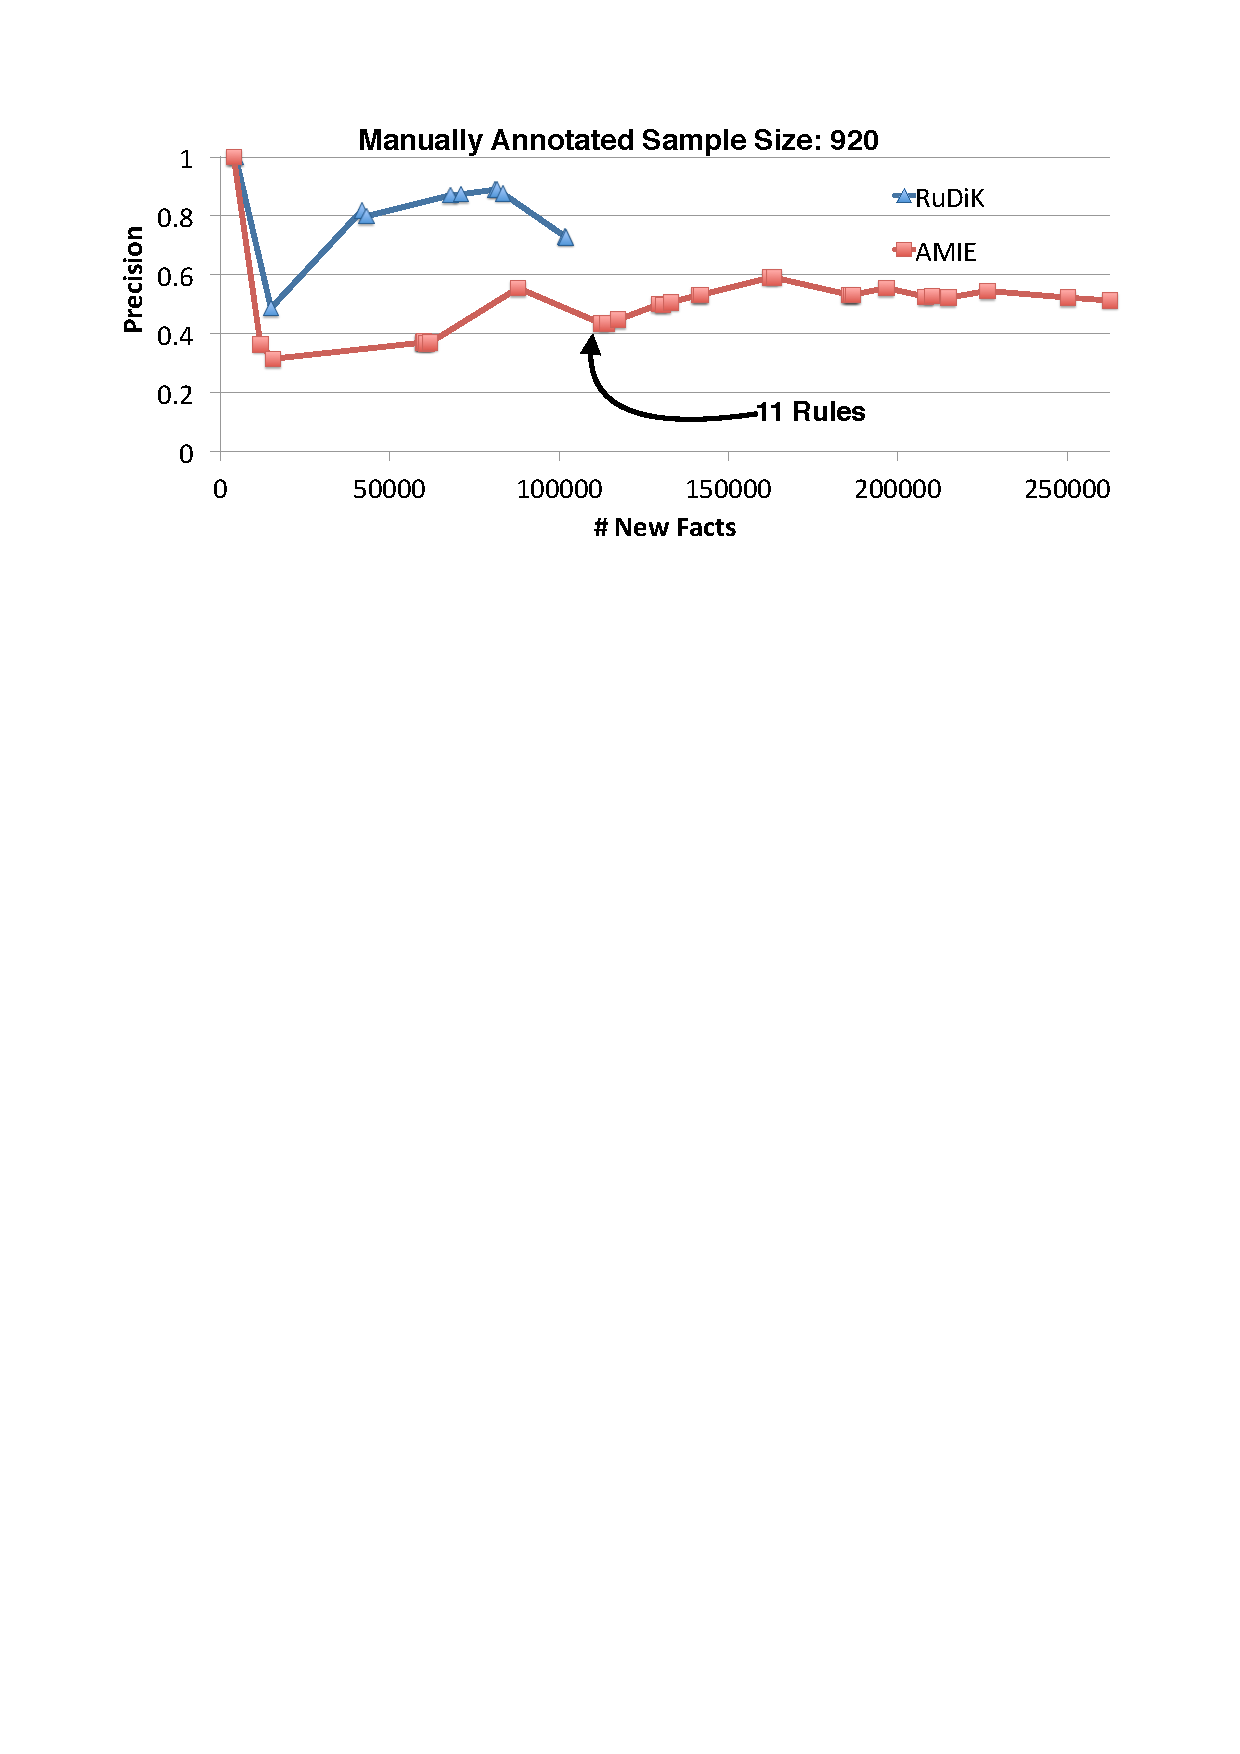
\includegraphics[width=.9\columnwidth]{include/figure/vsAmieYago.pdf}
	\vspace{-2ex}
	\caption{Accuracy for new facts identified by executing rules according to descending score on  \yago (no literals).}
	\label{fig:vs_amie_yago}
\end{figure}


\amie discovers 
%a huge amount of rules 
%along with their scores 
75 output rules in \yago, and 6090 in \dbpedia. We followed their experimental setting and picked the first 30 best rules according to their score. We then picked the rules produced by our approach on the same head predicate of the 30 best rules in the output of \amie. 
%I DON T UNDERSTAND LAST SENTENCE

\begin{figure}[ht]
	\centering
	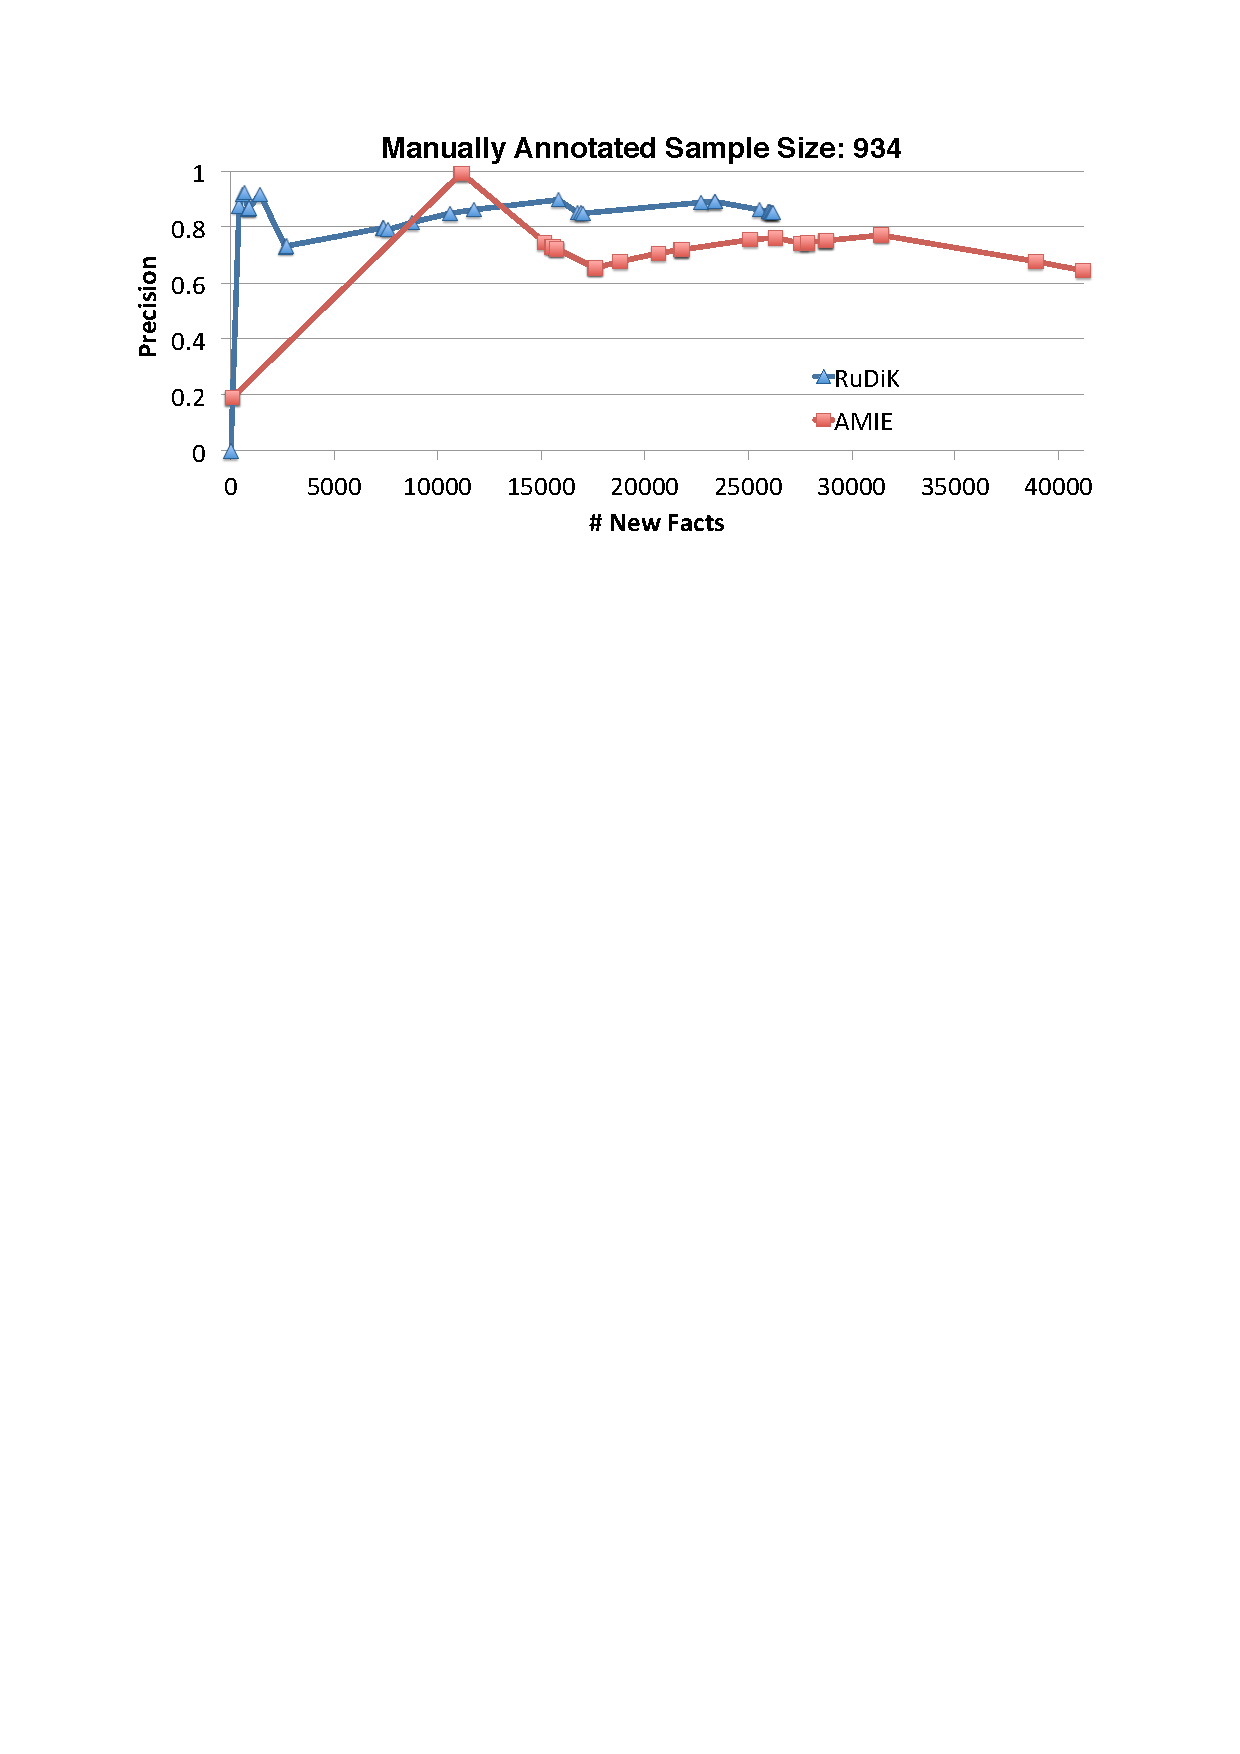
\includegraphics[width=.9\columnwidth]{include/figure/vsAmieDBPedia.pdf}
	\vspace{-2ex}
	\caption{Accuracy for errors identified by executing rules according to descending score on \dbpedia (no literals).}
	\label{fig:vs_amie_dbpedia}
\end{figure}

For this evaluation, we plot the total cumulative number of new unique predictions (x-axis) versus the aggregated precision (y-axis) when incrementally including in the solution the rules according to their descending score. Figures~\ref{fig:vs_amie_yago} and \ref{fig:vs_amie_dbpedia} report the results
on \yago and \dbpedia, respectively. 
Rules from \amie produce more predictions, but with a significant lower accuracy in both KBs. This is because, many good rules are preceded by meaningless ones in the ranking, and it is not clear how to set a proper $k$ to get the best top $k$ rules. 
In \krd, instead of the conventional ranking mechanism, we use a scoring function that discovers only inherently meaningful rules with enough support. 
%This approach is beneficial for the discovery, as shown  by the high precision we obtain %with a concise rule set 
%in both \yago and \dbpedia.
%
%\krd does not rely on a threshold and its algorithm identifies some of the cases when meaningful rules do not exist. % and it outputs a rule only when it has a strong confidence.
%is more conservative and produces much less rules than \amie. We noticed that for every predicate \amie always discovers more than one rule, while there are several predicates where the output of our algorithm is empty since none of the plausible rules has enough support. 
As a consequence, \krd outputs just 11 rules for 8 target predicates on the entire \yago -- for the remaining predicates \krd does not find any rule with enough support. If we limit the output of \amie to the best 11 rules in \yago (same output as our approach), its final accuracy is still 29\% below our approach, with just 10K more predictions.
%The only point where \amie outperforms our approach is upon \dbpedia when we consider the top $3$ rules: the third rule discovered by \amie is indeed a universally true rule that produces more than 11K correct predictions.
%NOT ESSENTIAL
%The precision of each rule is computed as described above with a minor modification: whenever a rule is unknown with its new predictions, we first check the existence of the new induced facts in a newer version of the KB. This is possible because the \amie dataset does not contain the most up to date versions. If a new fact does not appear neither in a newer version nor on the Web, it is evaluated as false.




%The $n$-th point from the left represents the total number of predictions and the total precision of these predictions, computed over the first $n$ rules (sorted according to \amie's score). 
%\amie produces many more predictions (262K vs 102K), but with a significant lower accuracy contrary to \krd which maintains a precision above 85\% before the last rule, with more than 80K predictions. This is due to the high number of rules in output of \amie, but also to the way these rules are ranked.

%NOT ESSENTIAL
%Moreover, our approach can also simulate \amie if we are more interested in recall. By modifying the $\alpha$ and $\beta$ parameters, we can obtain a higher number of predictions in output, at the expense of accuracy. 



%Figure~\ref{fig:vs_amie_dbpedia} shows the same evaluation on \dbpedia. \dbpedia has a richer set of relations, therefore also \krd is capable of producing 30 rules in output. Despite the same number of rules, once again our approach leads to a lower number of predictions (26K vs 41K) with a significant higher accuracy (85\% vs 74\%). The only point where \amie outperforms our approach is when we consider the top $3$ rules: the third rule discovered by \amie is indeed a universally true rule that produces more than 11K correct predictions.

\myparagraph{Negative Rules Comparison}
%We used \amie also to discover negative rules. 
\amie is not designed to discover negative rules, and can mine rules only for predicates explicitly stated in the KB. To use it as a baseline, we created a set of negative examples as explained in Section~\ref{sec:ex_generation} for each predicate in the top-5. To let \amie mine this information, for each negative example we added a new fact to the KB by connecting the two entities with the \emph{negation} of the predicate. 
For example, we added a \texttt{notSpouse} predicate connecting each pair of people who are not married according to our generation technique. We then run \amie on these new predicates. 
%The evaluation of negative rules is then carried out as explained before: we generate potential errors in the KB, and we manually evaluated the precision of such errors. 

\begin{table}[htb]
%\vspace{-3ex}
	\centering
	\caption{Negative Rules vs \amie.}
	\label{tab:vs_amie_neg}
	\begin{small}
		\begin{tabular}{c|c|c|c|c|}
			\cline{2-5}
			& \multicolumn{2}{c|}{{\amie}} & \multicolumn{2}{c|}{{\krd} (no literals)} \tabularnewline
			\hline
			\multicolumn{1}{ |c| }{\it KB}&{\it \# Errors} & {\it Precision} &{\it \# Errors} & {\it Precision} \tabularnewline
			\hline
			\multicolumn{1}{ |c| }{\dbpedia} & 457 (157) & 38.85\% & 148 (73) & \textbf{57.76}\%\tabularnewline
			\multicolumn{1}{ |c| }{\yago} & 633 (100) & 48.81\% & 550 (35) & \textbf{68.73}\%\tabularnewline
			\hline
		\end{tabular}
	\end{small}
\end{table}


Table~\ref{tab:vs_amie_neg} shows that \krd outperforms \amie in both cases with a precision gain of almost 20\%. The drop in quality for \krd w.r.t. the ones showed in Section~\ref{sec:gen_evaluation} is because we are using %the \amie modified 
KBs without literals.
Numbers in brackets show the number of triples manually annotated. 
% This is because for the negation of a predicate, we use the actual predicate as counter examples. \amie instead is not aware that the actual predicate provides counter examples for the negation of it, hence it is much less precise. In fact the output of \amie consists in a high number of rules for each predicate (often more than 30), and in many cases \amie produces same rules for both positive and negative scenarios. 
%As an example, \amie outputs that if a country $a$ exports a good $b$, then $a$ imports $b$ and $a$ does not import $b$. 

%NOT ESSENTIAL
%Despite clearly outperforming \amie, numbers look significantly lower that the ones showed in Section~\ref{sec:gen_evaluation}. This is because we are using the \amie modified KBs which do not contain literals. As explained earlier, literals play a vital role when discovering negative rules, both in terms of total errors discovered and in terms of precision. Excluding literals is a big disadvantage, and we will emphasise this aspect in detail in Section~\ref{sec:krd_int_evaluation}. (TO DO: check if the internal evaluation actually exists)

\myparagraph{Running Time}
%We report the running time of \amie compared to our approach. 
Running times for \amie are different from~\cite{galarraga2015fast}, where it was run on a 48GB RAM server. On our machine, \amie could finish the computation  on \yago 2, while for other KBs it got stuck after some time. For these cases, we stopped the computation if there were no changes in the output for more than 2 hours.

%HERE WE DO NOT REPORT THE KB SIZE OTHERWISE THE TABLE IS TOO BIG
%\begin{table}[t]
%	\centering
%	\caption{Run Time vs \amie.}
%	\label{tab:amie_runtime}
%	\begin{small}
%		\begin{tabular}
%			{|c|c|c|c|c|c|}
%			\hline
%			\hline
%			{\it KB}&{\it\#Triple}&{\it\#Predicates}&{\it\amie}&{\it\krd}&{\it Types}\tabularnewline
%			\hline
%			\yago 2& 948.3K & 20 & 30s & 18m,15s & 12s \tabularnewline
%			\yago 2s& 4.1M & 26 (38)& $>8$h & 47m,10s & 11s  \tabularnewline
%			\dbpedia 2.0& 7M & 904 (10342)& $>10$h & 7h,12m & 77s  \tabularnewline
%			\dbpedia 3.8& 11M & 237 (649) & $>15$h & 8h,10m & 37s  \tabularnewline
%			\wikidata & 8.4M & 118 (430) & $>25$h & 8h,2m & 11s  \tabularnewline
%			\yago 3*& 88.3M & 72 & - & 2h,35m & 128s  \tabularnewline
%			\hline
%		\end{tabular}
%	\end{small}
%\end{table}
\begin{table}[htb]
%\vspace{-3ex}
	\centering
	\caption{Run Time vs \amie.}
	\label{tab:amie_runtime}
	\begin{small}
		\begin{tabular}
			{|c|c|c|c|c|}
			\hline
			\hline
			{\it KB}&{\it\#Predicates}&{\it\amie}&{\it\krd}&{\it Types}\tabularnewline
			\hline
			\yago 2& 20 & 30s & 18m,15s & 12s \tabularnewline
			\yago 2s& 26 (38)& $>8$h & 47m,10s & 11s  \tabularnewline
			\dbpedia 2.0& 904 (10342)& $>10$h & 7h,12m & 77s  \tabularnewline
			\dbpedia 3.8& 237 (649) & $>15$h & 8h,10m & 37s  \tabularnewline
			\wikidata & 118 (430) & $>25$h & 8h,2m & 11s  \tabularnewline
			\hline
			\yago 3*& 72 & - & 2h,35m & 128s  \tabularnewline
			\hline
		\end{tabular}
	\end{small}
\end{table}

Table~\ref{tab:amie_runtime} reports the running time on different KBs. The first five KBs are \amie modified versions, while \yago 3* is complete \yago, including literals and \texttt{rdf:type}. 
The second column shows the total number of predicates for which \amie produced at least one rule before getting stuck, while in brackets we report the total number of predicates in the KB.
%????analyzed<<<<<<<<CORRECT?<<<<<<<<<<'
%
%for which \amie was able to produce at least one rule. In some cases \amie got stuck without producing any rules for some predicates, hence we report the total number of predicates in brackets. 
%For a fair comparison we run our algorithm only on those predicates for which \amie could produce at least one rule. 
The third and fourth columns report the total running time of the two approaches. Despite being disk-based, \krd successfully completes the task faster than \amie in all cases, except for \yago 2. This is because of the very small size of this KB, which fits in 
%main 
memory. However, when we deal with complete KBs (\yago 3*), the KB could not even be loaded due to out of memory errors. The last column reports the running time to compute \texttt{rdf:type} information for all predicates in the KB. 
%This time is negligible w.r.t. the total running time. 
%The running time justifies our disk-based strategy: \krd can successfully discover rules for any size KB on any machine.

\myparagraph{Other Systems}
We found other available systems to discover rules in KBs. In~\cite{abedjan2014amending}, the system discovers %new facts at the instance level, hence 
rules that are less general than our approach; on \yago 2, it discovers 2K new facts with a precision lower than 70\%, while the best rule we discover on \yago 2 already produces more than 4K facts with a 100\% precision. 
%are we using the same KB? 
A recent system~\cite{Chen:2016} implements \amie algorithm with a focus on scalability. They do not modify the mining part, but split the KB into multiple cluster nodes to run in parallel. The output is the same as \amie. We did not compare with classic Inductive Logic Programming systems~\cite{dehaspe1999discovery}, as these are already significantly outperformed by \amie both in accuracy and running time.

\vspace{-1ex}
\subsection{Machine Learning Application} \label{sec:krd_deep_dive}
\vspace{-1ex}
The main goal of this set of experiments is to demonstrate the applicability of our approach in providing Machine Learning (ML) algorithms meaningful training examples.
We chose \deepdive~\cite{shin2015incremental}, a ML framework to construct KBs. \deepdive extracts entities and relations from text articles via distant supervision. The key idea behind distant supervision is to use an external source of information (e.g., a KB) to provide training examples for a supervised algorithm. For example, \deepdive can extract mentions of married couples from text documents. In such a scenario \deepdive uses as a first step \dbpedia to label some pairs of entities as \emph{true} positive (those pairs of married couples that can be found in \dbpedia). 
%These labelled examples are then used to construct a factor graph, similar to Markov Logic, that will predict labels on the rest of candidates. 
Unfortunately, KBs directly provide positive examples only. Hence in \deepdive the burden of creating negative examples is left to the user. % through manual rules definition.

\begin{figure}[b]
	\centering
	\vspace{1ex}
	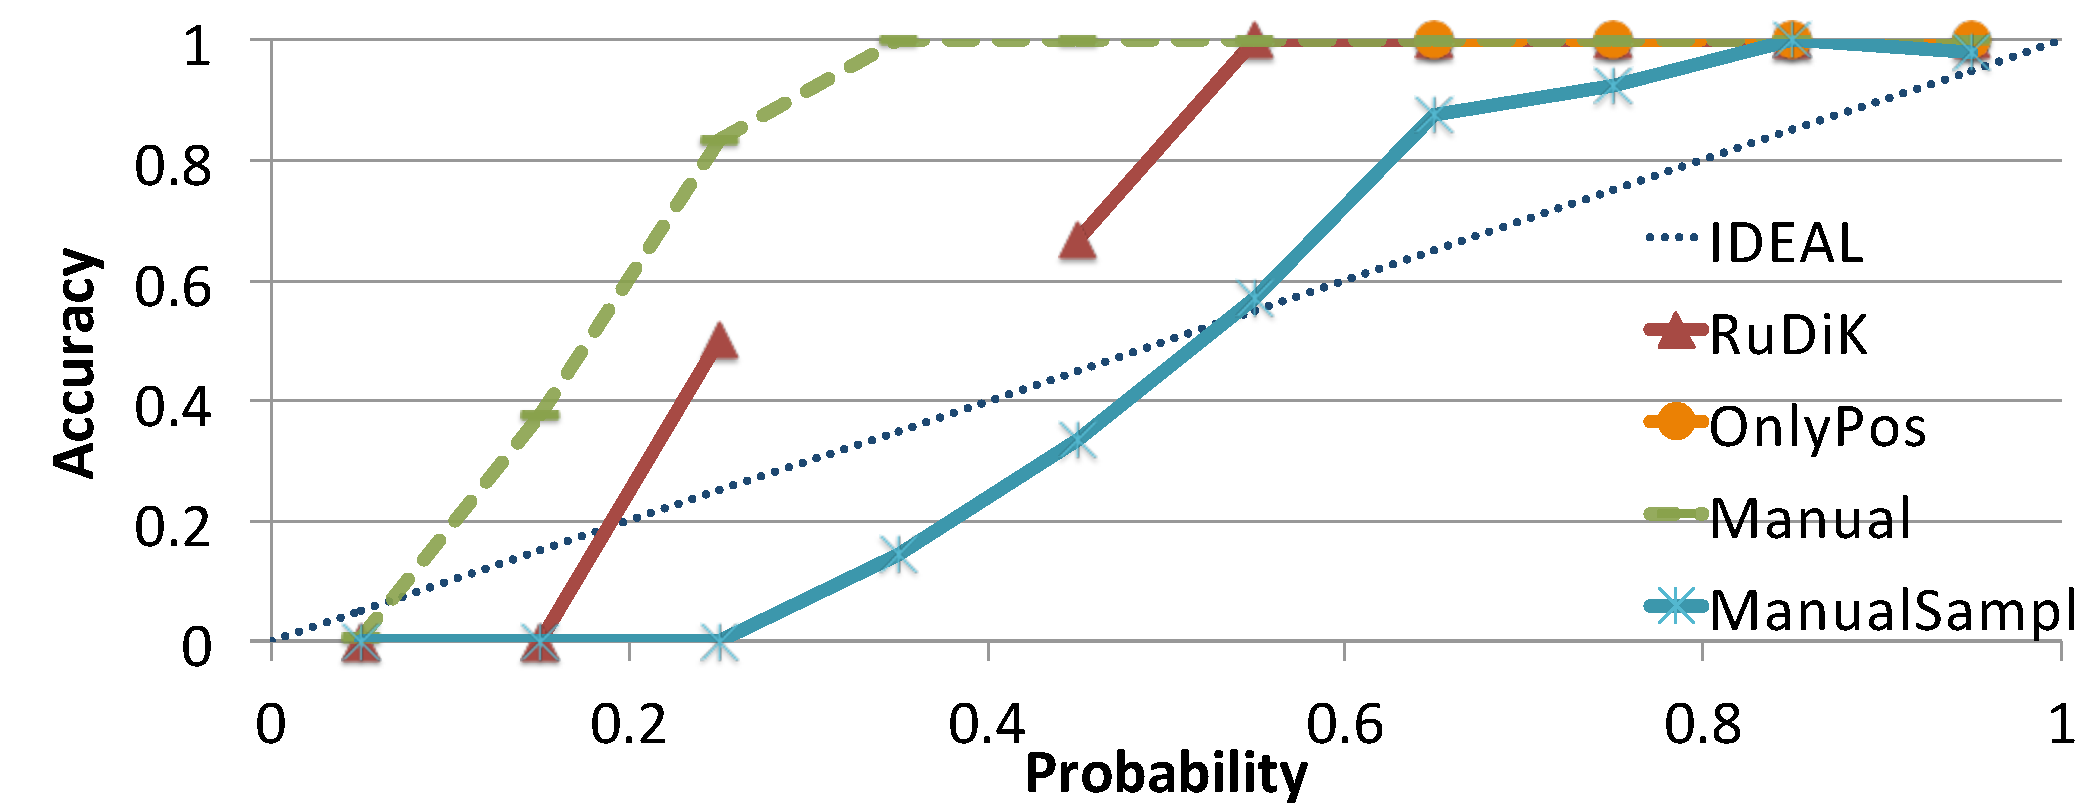
\includegraphics[width=.95\columnwidth]{include/figure/deepDive1K.pdf}
	\vspace{-1ex}
	\caption{\deepdive execution with 1K articles.}
	\label{fig:deep_dive_1k}
\end{figure}

In this set of experiments, we created negative examples with the rules obtained on \dbpedia with \krd. We then compared the output of \deepdive upon its spouse example trained with different sets of negative examples.
%\footnote{\url{http://deepdive.stanford.edu/}}, where the goal is to extract mentions of married people from text articles
 %We used \deepdive spouse showcase example. \deepdive already provides some negative rules to generate negative examples (e.g., if two people appear in a sentence connected by the words \textit{brother} or \textit{sister} then they are not married). We therefore compare the output of \deepdive using our generated negative examples and the ones generated with \deepdive rules. 

Figure~\ref{fig:deep_dive_1k} shows \deepdive accuracy plot run on 1K input documents. The accuracy plot shows the fraction of correct positive predictions over total predictions (y-axis), for each output probability value (x-axis). The perfect algorithm, marked by the dotted blue line, would predict all facts with a probability of 1 and zero facts with an output probability of 0.
% which is the idealistic expected behavior marked by the dotted blue line. 
The best algorithm deflects the least from the blue dotted line, and this is our evaluation metric.
%The dotted blue line represents the ideal situation, where the system finds high number of evidence positive predictions for higher probability output values -- when the output probability is 0 there should not be positive predictions. 
%The plot is computed over a test set, while the system is trained over a separated training set. 
The figure shows 4 lines other than the ideal one. \krd is the output of \deepdive using our approach to generate negative examples. \texttt{OnlyPos} uses only positive examples from \dbpedia, \texttt{Manual} uses positive examples from \dbpedia and manually defined rules to generate negative examples, while \texttt{ManualSampl} uses only a sample of the manually generated negative examples in size equal to positive examples. We observe that \texttt{OnlyPos} and \texttt{Manual} do not provide valid training, as the former has only positive examples and labels everything as true, while the latter has many more negative examples than positive and labels everything as false. \texttt{ManualSampl} is the clear winner, while our approach suffers from the absence of data: over the input 1K articles, we could find only 20 positive and 15 negative examples from \dbpedia.
The lack of evidence in the training data also explains the missing points for \krd in the chart, where there were no predictions in the probability range 25-45\%.

\begin{figure}[t]
	\centering
	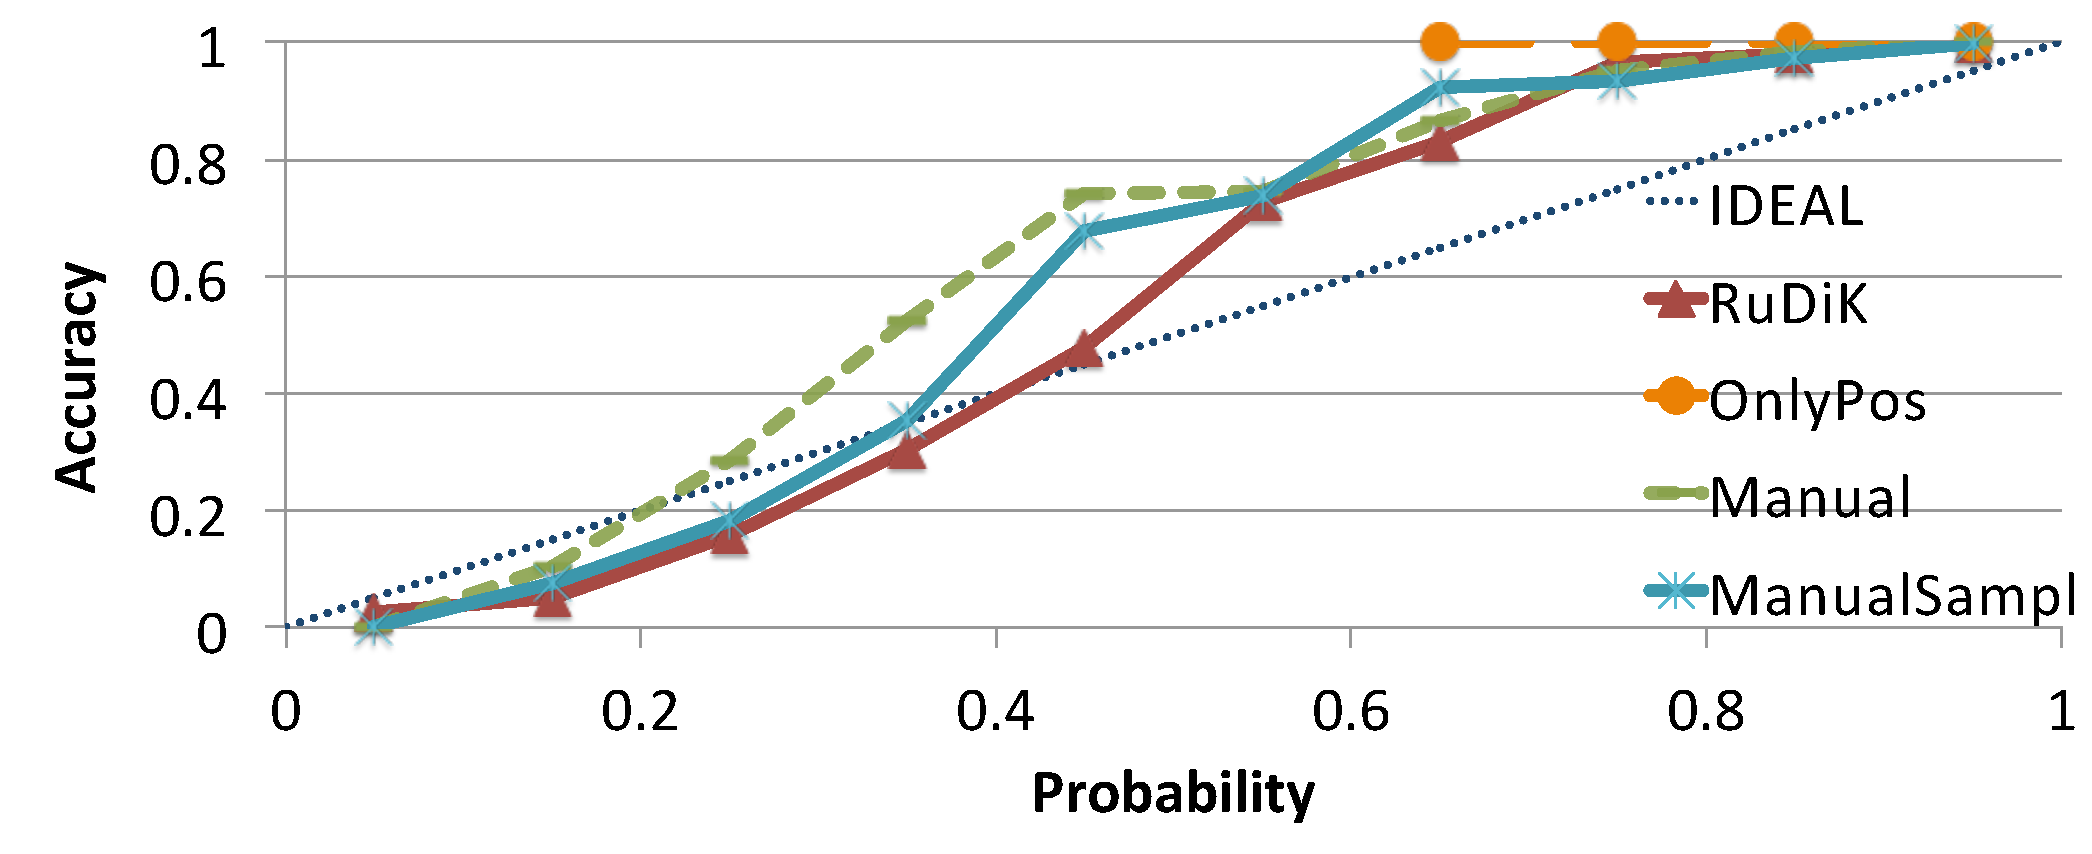
\includegraphics[width=.95\columnwidth]{include/figure/deepDive1M.pdf}
		\vspace{-1ex}
	\caption{\deepdive execution with 1M articles.}
	\label{fig:deep_dive_1M}
\end{figure}

When we extend the input to 1M articles, things change drastically (Figure~\ref{fig:deep_dive_1M}). All the three approaches except \texttt{OnlyPos} can successfully drive \deepdive in the training, with the examples provided with \krd leading to a slightly better result. This is because of the quality of the negative examples: our rules generate representative examples that help \deepdive in understanding discriminatory features between positive and negative labels.
The output of \texttt{ManualSampl} and \krd are very similar, meaning that we can use our approach to simulate user behaviour and provide negative examples at zero cost. 
%NOT ESSENTIAL
%With manually defined rules the number of generated examples is significantly higher ($23$K vs $5$K generated with \krd), however the results are very similar since a small number of significant examples is enough to provide complete evidence for the training. 
%This confirms the main finding of this experiment: as long as we have an external source of information with a decent coverage over the input articles, users do not need to worry about providing rules to generate negative examples.

\vspace{-1ex}
\subsection{Internal Evaluation} ~\label{sec:krd_int_evaluation}
In this last section we sketch the impact of individual components in \krd.
Full results on the internal evaluation are not reported due to space reasons but can be found in the technical report online at \url{http://bit.ly/2bDZO9F}.

Here we briefly outline some of the most relevant findings. 
\begin{inparaenum}[\itshape 1)]
	\item We show the benefits of including literals in the mining especially for negative rules, where we double the number of errors discovered with a 10\% increase in precision.
	\item We show that $3$ is the optimal value for the $maxPathLen$ parameter: with smaller values we lose several meaningful rules, and with bigger values we do not gain in precision. % or errors detected.
	\item We empirically validate the choices of $\alpha$ and $\beta$ for both positive and negative settings.
	\item We demonstrate the validity of our LCWA-based generation of negative examples, which clearly outperforms random generation strategies in terms of accuracy.
	\item We quantify the benefits of $A^*$ search algorithm and pruning, where on an average the running time is halved with peaks of an order of magnitude.
	\item We show the increase in precision of our set cover problem formulation w.r.t. a ranking based solution. Correct rules oftentimes are not among the top-10 ranked, and we show cases where meaningful rules are below the 100$^{th}$ position.
	
	%there exist good rules ranked as low as the hundreds (e.g., a good rule 120$^{th}$ in the ranking). 
	%stefano please check this number <<<<
	%This emphasize upon the fragility in ranking mechanisms.
\end{inparaenum}
%CANNOT AFFORD TO INCLUDE ALL INTERNATAL EVALUATION
%In this last set of experiments we measured the impact of \krd relevant features in order to quantify the benefit of three main aspects in rule discovery. 
%We run \krd on \dbpedia with different settings than the standard ones.
%We report results on the same top-5 predicates of Section~\ref{sec:gen_evaluation} for both positive and negative rules.
%
%\myparagraph{Effect of Literals}
%Since previous KB rule discovery approaches exclude literals from the mining~\cite{abedjan2014amending,galarraga2015fast} (TODO: cite Sigmod ontological), we wanted to quantify the impact of having literal rules. Thus we run \krd excluding all literal values. Table~\ref{tab:literals_effect} reports the output precision with and without literals.
%\begin{table}[b]
%	\centering
%	
%	\begin{small}
%		\begin{tabular}{c|c|c|c|c|}
%			\cline{2-5}
%			& \multicolumn{2}{c|}{\textbf{With Literals}} & \multicolumn{2}{c|}{\textbf{Without Literals}} \tabularnewline
%			\hline
%			\multicolumn{1}{ |c| }{\it Type}&{\it Run Time} & {\it Precision} &{\it Run Time} & {\it Precision} \tabularnewline
%			\hline
%			\multicolumn{1}{ |c| }{Positive Rules} & $\sim$35min & \textbf{63.99}\% & $\sim$54min & 60.49\%\tabularnewline
%			\multicolumn{1}{ |c| }{Negative Rules} &  $\sim$20min & \textbf{92.38}\% (499) &$\sim$25min &84.85\% (235) \tabularnewline
%			\hline
%		\end{tabular}
%	\end{small}
%	\caption{Rules Accuracy without Literals on \dbpedia.}
%	\label{tab:literals_effect}
%\end{table}
%Including literal values in the mining has a considerable impact on final accuracy, both for positive and negative rules. The effect is particularly evident for negative rules, where excluding literals involves finding less than half potential errors (numbers in brackets) with a lower precision. \texttt{founder} is the most evident example: \krd discovers 79 potential errors with a 95\% precision with literal rules, while there are not output errors with rules without literals.
%
%Surpisingly, including literals reduces also the running time. This is due to the pruning effect of the $A^*$ search: if we include literals the algorithm can find rather soon valid literal rules, which causes the pruning of several paths on the graph. If we exulted literals instead these paths cannot be pruned and needs to be inspected by the algorithm, which entails a bigger search space.
%
%\myparagraph{Rules Length Impact}
%The $maxPathLen$ parameter fixes the maximum number of atoms allowed in the body of a rule. Low values for $maxPathLen$ may exclude from the search space meaningful rules, while high values may exponentially increase the search space and consequently the running time. Table~\ref{tab:rules_len_impact} reports
%\begin{table}[htt]
%	\centering
%	\caption{$maxPathLen$ Parameter Impact on \dbpedia.}
%	\label{tab:rules_len_impact}
%	\begin{small}
%		\begin{tabular}{c|c|c|c|c|c|c|}
%			\cline{2-7}
%			& \multicolumn{2}{c|}{$MaxPathLen$ = \textbf{2}} & \multicolumn{2}{c|}{$MaxPathLen$ = \textbf{3}} & \multicolumn{2}{c|}{$MaxPathLen$ = \textbf{4}}\tabularnewline
%			\hline
%			\multicolumn{1}{ |c| }{\it Type}&{\it Run Time} & {\it Precision} &{\it Run Time} & {\it Precision} &{\it Run Time} & {\it Precision} \tabularnewline
%			\hline
%			\multicolumn{1}{ |c| }{Positive} & \textbf{$\sim$3min}& 49.17\% & $\sim$35min & \textbf{63.99}\% & & \tabularnewline
%			\multicolumn{1}{ |c| }{Negative} & \textbf{$\sim$56sec} & 90\% (131) & $\sim$20min & \textbf{92.38}\% (499)& & \tabularnewline
%			\hline
%		\end{tabular}
%	\end{small}
%\end{table}
%accuracy values and run times for different $maxPathLen$ settings. If we set $maxPathLen=2$ we observe a significant improvement in running time, at the expense of loosing several meaningful rules. In particular we loose all the rules that involve literals comparison, as these require a minimum of three atoms in the body. This is particularly evident for negative rules, where we spot a fewer number of errors (in round brackets) with a lower precision. At the other side of the spectrum, with $maxPathLen=4$ the search space explodes and \krd was not capable of finishing the computation within 24 hours for each predicate. We therefore report the accuracy of rules discovered in 24 hours of computation. The results are comparable to those computed with $maxPathLen=3$, provided the absence of rules that might have been discovered after 24 hours. Furthermore, we did not notice any new discovered correct rule with body length equal to 4. Rules with length 4 are usually very complex to understand, and when executed over the KB they often return an empty result (i.e., they are useless both for discovering additional information and for identifying inconsistencies). Here a couple of examples of output rules with length 4:
%
%%NOT ESSENTIAL
%%\vspace{-5ex}
%%{\scriptsize
%%	\begin{gather*}
%%		\atom{birthPlace}{a}{v_0} \wedge \atom{areaTotal}{v_0}{v_1} \wedge \atom{viafId}{b}{v_2} \wedge v_1 < v_2 \Rightarrow \neg \atom{academicAdvisor}{a}{b} \\
%%		\atom{foundingYear}{a}{v_2} \wedge \atom{birthPlace}{b}{v_0} \wedge \atom{foundingYear}{v_1}{v_2}  \wedge \atom{foundationPlace}{v_1}{v_0} \Rightarrow \atom{founder}{a}{b}
%%	\end{gather*}
%%}
%%We therefore decided that $maxPathLen=3$ is a good compromise between a reasonable running time and a good output accuracy.
%
%\myparagraph{Negative Examples Generation}
%A key point in \krd is the generation of negative examples with a modified version of the LCWA (Section~\ref{sec:ex_generation}). We therefore evaluate two different strategies to generate negative examples. Given a target predicate $p$ from a KB $\kb$, we call $t_a$ the most common type of entities that are subject of $p$, and $t_b$ the most common type for the object. As an example, if $p=$\texttt{founder}, $t_a=Company$ and $t_b=Person$. We define $k$ as the number of triples having $p$ as predicate in $\kb$ -- $k$ is the cardinality of the positive examples set. The first alternative negative examples generation strategy is \emph{Random}: we randomly select $k$ pairs $(x,y)$ from the cartesian product of all entities $x$ of type $t_a$ and all entities $y$ of type $t_b$, such that the triple $\<x,p,y\> \notin \kb$. The second generation strategy, named ${LCWA}\_Random$, leverages on the LCWA. In $LCWA\_Random$ we randomly pick $k$ pairs $(x,y)$ from the cartesian product of all entities $x$ of type $t_a$ and all entities $y$ of type $t_b$, such that:
%\begin{inparaenum}[\itshape(i)]
%	\item $\<x,p,y'\> \in \kb$, with $y' \neq y$;
%	\item $\<x',p,y\> \in \kb$, with $x' \neq x$;
%	\item $\<x,p,y\> \notin \kb$.
%\end{inparaenum}
%$LCWA\_Random$ is equivalent to \krd generation strategy, minus the constriction that $x$ and $y$ must be connected by a predicate different from $p$. The constraint of having $k$ examples aims at reducing the size of the cartesian product that can easily explode otherwise.
%
%Table~\ref{tab:random_neg_examples} reports the accuracy of discovering negative rules with the three different generation strategies (\krd is our modified LCWA strategy).
%\begin{table}[t]
%	\centering
%	\caption{Effect of Negative Examples Generation Strategy on \dbpedia.}
%	\label{tab:random_neg_examples}
%	\begin{tabular}{|c|c|c|c|c|}
%		\hline
%		\hline
%		{\it Strategy}&{\it \# Potential Errors} & {\it Precision} \tabularnewline
%		\hline
%		\emph{Random} & 247 & \textbf{95.95}\%\tabularnewline
%		\emph{LCWA\_Random} & 263 & 95.82\% \tabularnewline
%		\krd & \textbf{499} & 92.38\%\tabularnewline
%		\hline
%	\end{tabular}
%\end{table}
%\emph{Random} and \emph{LCWA\_Random} strategies show very similar behaviours, with a slightly better precision than \krd. This is because whenever we randomly pick examples from the cartesian product of subject and object, the likelihood of picking entities from a different time period is very high, and negative rules pivoting on time constraints are usually correct.
%As an example, a correct rule for the target predicate \texttt{child} is $\atom{birthDate}{a}{v_0} \wedge \atom{birthDate}{b}{v_1} \wedge v_0 > v_1 \Rightarrow \neg \atom{child}{a}{b}$, stating that whenever a person $a$ is born after a person $b$, then $b$ cannot be child of $a$.
%The likelihood of randomly picking some pairs of persons $(x,y)$ where $x$ is born after $y$ is very high, hence such kind of rules will often be discovered. However these are the \emph{only} kind of rules that random generation strategies are able to find, as shown from the smaller number of errors that they can identify. 
%Instead, the constriction of forcing $x$ and $y$ to be connected by a different predicate generates  negative examples with heterogeneous properties that lead to different results. Rules such as $\atom{parent}{a}{b} \Rightarrow \neg \atom{spouse}{a}{b}$ are very unlikely to be generated with random strategies, since the likelihood of picking two people that are in a parent relation is very low. The generation strategy we adopt in \krd allows the discovery of more types of rules, and not only rules involving time constraints. This has multiple benefits: on the one hand, we discover more rules, which entails discovering a higher number of errors (Table~\ref{tab:random_neg_examples}); on the other hand, different rule types lead to high quality negative examples, that can be used in several applications such as training Machine Learning algorithms (see Section~\ref{sec:krd_deep_dive}).
%
%\myparagraph{Effect of Weight Parameters}
%\begin{figure}[t]
%	\centering
%	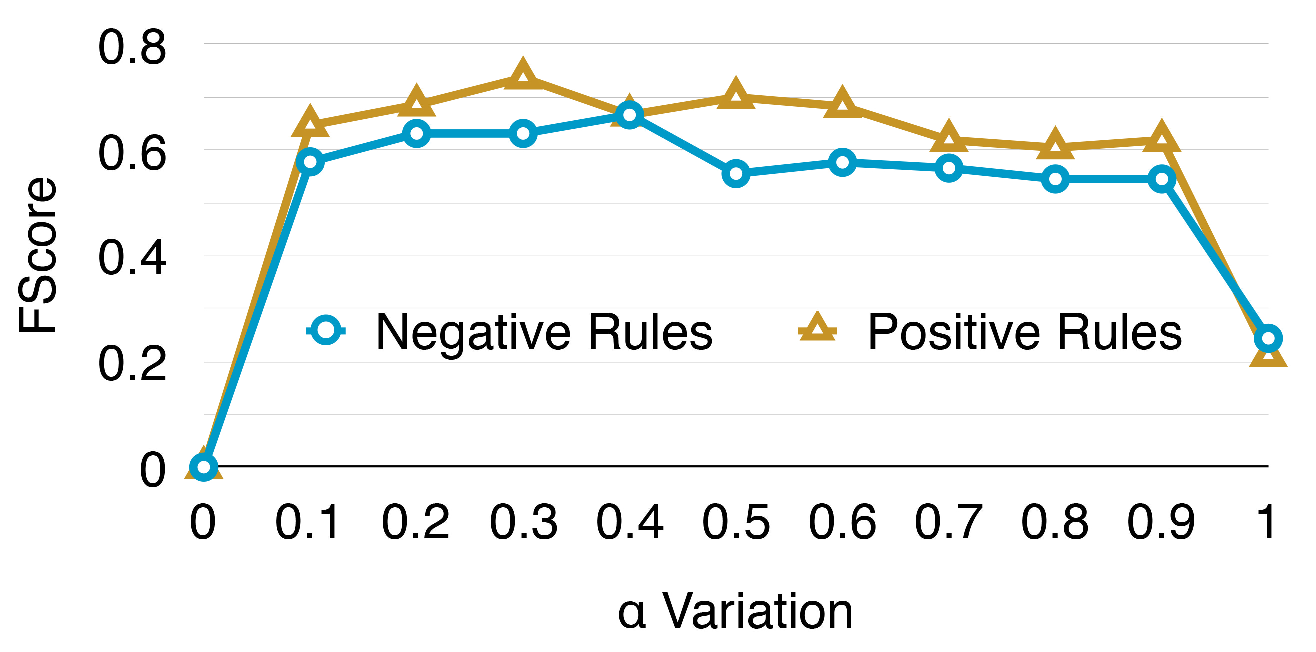
\includegraphics[width=0.9\columnwidth]{include/figure/alpha_impact.pdf}
%	\caption{$\alpha$ Parameter Performance Impact}
%	\label{fig:alpha_impact}
%\end{figure}
%Our weight function is ruled by two different parameters: $\alpha$ and $\beta$, with $\alpha \in [0,1]$ and $\beta=1-\alpha$ (Section~\ref{sec:krd_weight_fun}). This experiment aims at establishing the optimal value to assign to $\alpha$ and $\beta$, and to quantify the impact of the two parameters on the overall performance. We recall that $\alpha$ quantifies the relevance of the coverage over the generation set, while $\beta$ is the importance of the coverage over the validation set. In other words, a high $\alpha$ supports high recall over precision, while a high $\beta$ supports a high precision over recall. Figure~\ref{} shows the variation of \textsf{$F_1$-Score} with different values of $\alpha$ for both positive and negative rules on \dbpedia. For each different run, we manually label each output rule as true or false, where the total number of correct rules for each predicate is the union of all possible correct rules over all the runs. We then compute \textsf{Precision}, \textsf{Recall}, and \textsf{$F_1$-Score} at rule level. On the one hand, setting $\alpha=0$ produces an empty output, since we neglect the coverage over the generation set and we are just after rules that do not cover any element of the validation set. On the other hand, setting $\alpha=1$ means chasing rules just based on the coverage over the generation set, no matter what the coverage over the validation set is. This strategy ends up in producing a huge amount of rules (high recall), with very few correct rules (low precision). Correct values lie somewhere in between. For positive rules, the best assignment is $\alpha=0.3$ and $\beta=0.7$. Since discovering correct positive rules is more challenging than negative ones, favoring precision over recall gives the best accuracy. For negative rules instead, the best assignment is $\alpha=0.4$ and $\beta=0.6$. Since negative rules are often correct, we can relax the constraint over precision and be slightly more recall oriented. In both cases, the variation in performance for $\alpha \in [0.1,0.9]$ is anyway limited ($\leq 12\%$), showing the robustness of the set cover problem formulation.
%
%\myparagraph{$A^*$ pruning impact}
%\begin{figure}[b]
%	\centering
%	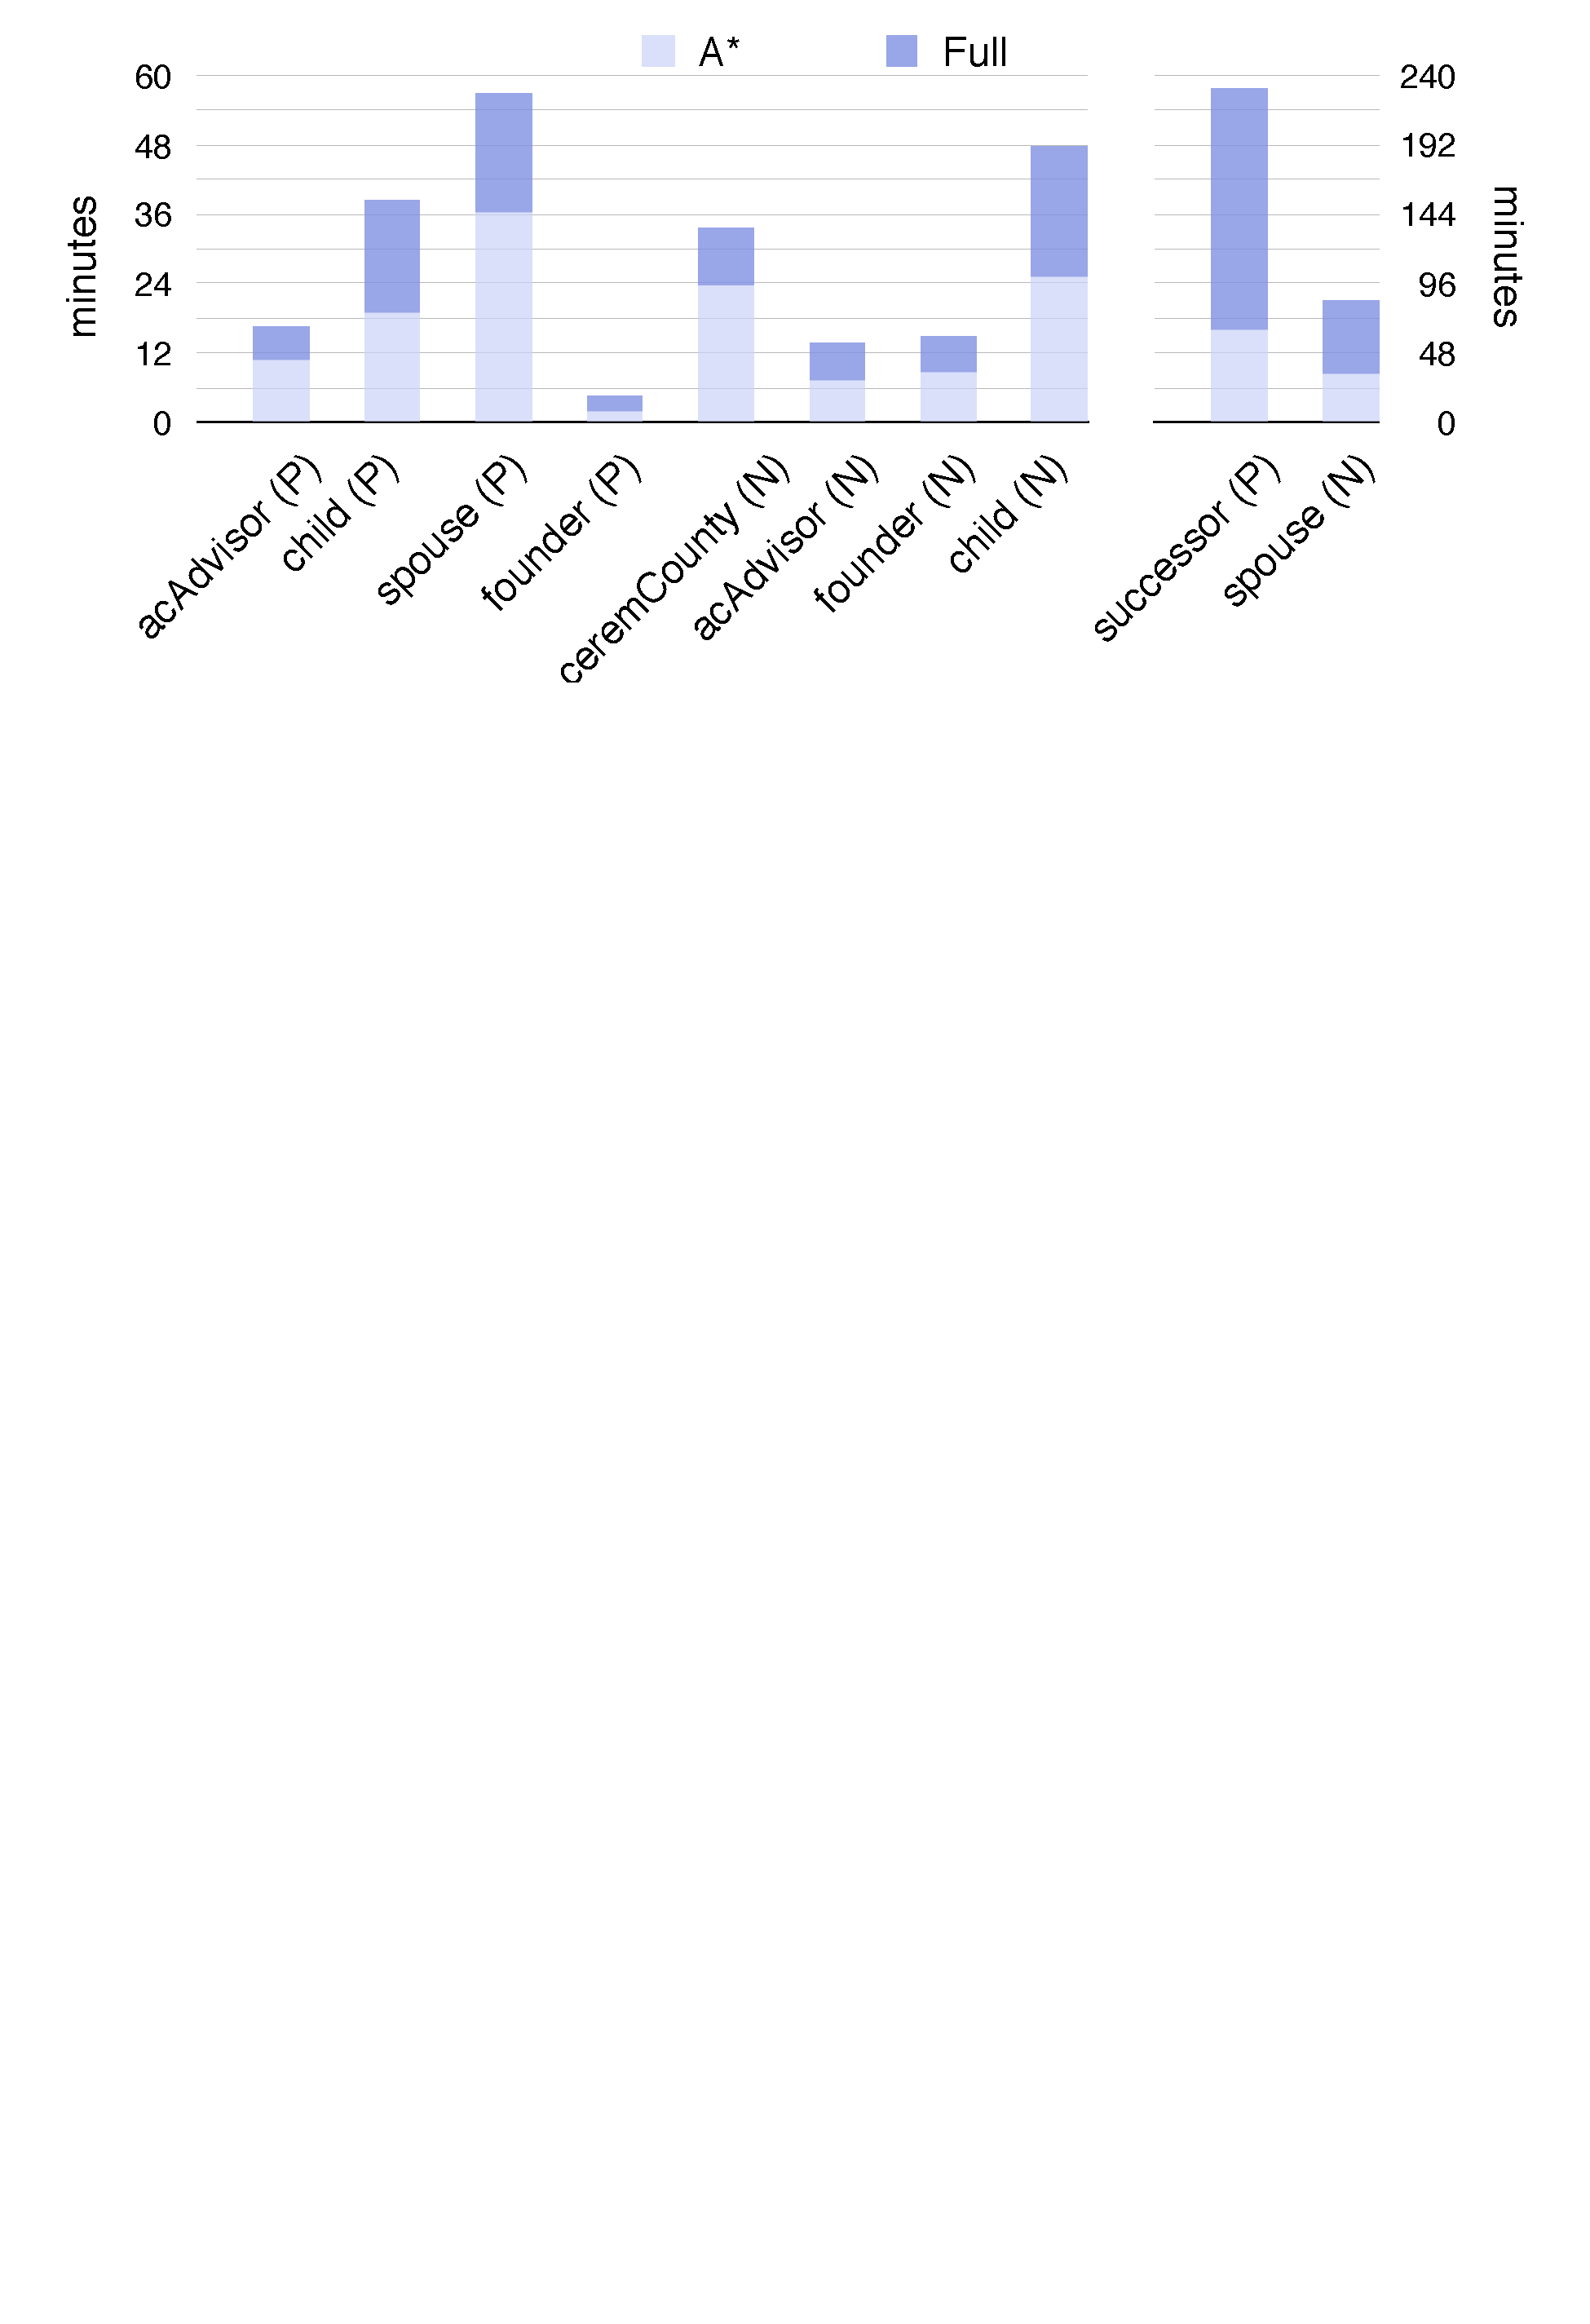
\includegraphics[width=\columnwidth]{include/figure/a*_runtime_improv.pdf}
%	\caption{$A^*$ Pruning Runtime Improvement}
%	\label{fig:pruning_impact}
%\end{figure}
%Another aspect we wanted to quantify is the benefit brought by the $A^*$ algorithm on the overall running time. Figure~\ref{fig:pruning_impact} shows the running time, for each target predicate, of the $A^*$ algorithm (light-colored bars) against a modified version that first generates the universe of all possible rules, and then apply the greedy set cover algorithm on such a universe (dark-colored bars). For the last two predicates refer to the y-axis labels on the right hand side, as these predicates have a significant higher running time. In the figure \texttt{(P)} refers to positive rules, while \texttt{(N)} to negative rules.
%The $A^*$ strategy allows the pruning of several unpromising paths and avoids the generations of such paths from the disk. This is directly reflected on running times, where we notice an average 50\% improvement. When there exist rules that cover many examples from the generation set (e.g., \texttt{successor (P)}, \texttt{founder (P)}), the algorithm is capable of identifying such rules rather early, thus pruning several unpromising paths that cover a subset examples from the generation set. In such cases the running time improvement is above 70\%.


\section{Related Work} \label{sec:krd_related}

Our work %is inspired by Inductive Logic Programming, but 
uses techniques from dependencies discovery in relational databases, KBs construction, and mining graph patterns. 
We review some of the most relevant works below.

%\myparagraph{Relational Database Constraints} 
A significant body of work has addressed the problem of discovering constraints over relational data. 
Due to the presence of a pre-defined schema, dependencies are discovered over the attributes and encoded into formalisms such as 
Functional Dependencies (FDs)~\cite{abiteboul1995foundations,huhtala1999tane,wyss2001fastfds}, Conditional FDs~\cite{fan2011discovering} 
and Denial Constraints (DCs)~\cite{chu2013discovering}. 
%
%It is interesting to note that the Our positive rules  to FDs while a close parallel can be drawn between our negative rules and DCs.
%
%Functional Dependencies (FDs), a formalism to express relations and dependencies among attributes, has been studied in constraints discovery literature for more than 20 years~\cite{abiteboul1995foundations}, with a recent focus on performance~\cite{abedjan2014dfd}. FDs can be grouped into two strands: the schema-level approaches~\cite{huhtala1999tane} (similar to our positive rules discovery), and the instance-driven approaches~\cite{wyss2001fastfds}. More recently, Conditional FDs extend standard FDs by enforcing patterns of semantically related constants~\cite{fan2011discovering}. In the context of inconsistencies discovery for relational data, Denial Constrains (DCs) are the current state-of-the-art techniques~\cite{chu2013discovering}. DCs are a universally quantified first order logic formalism to express constraints over relational data, and they are directly related to our negative output rules. Efficient DCs algorithms have been proposed for data cleaning and consistent query answering~\cite{bertossi2011database,chu2013holistic}. 
%Despite being directly related to our output and expressing a richer language, 
However, techniques for FDs and DCs discovery cannot be applied to RDF databases for three main reasons:
\begin{inparaenum}[\itshape(i)]
	\item the schema-less nature of RDF data and the open world assumption; % which no longer holds on RDF KBs;
	\item traditional approaches rely on the assumption that data is either clean or has a negligible amount of errors, which is not the case with KBs;
	\item even when the algorithms are designed to support more errors~\cite{abedjan2015temporal,kivinen1995approximate}, scalability issues on large RDF dataset: a direct application of relational database techniques on RDF KBs requires the materilization of all possible predicate combinations into relational tables.
\end{inparaenum}

%A few FD mining approaches like~\cite{abedjan2015temporal,kivinen1995approximate} that can work with erroneous datasets are still inapplicable to RDF data due to scalability problems.
Recently, Fan et. al.~\cite{FanFDGraphs} laid the theoretical foundations of Functional Dependencies on Graphs (GFDs). 
%They also propose parallel algorithms for GFDs computation and evaluate the accuracy on \yago and \dbpedia. Despite existing a natural correlation between FDs and Horn Rules, 
However, the language they propose covers only a portion of our negative rules to detect inconsistencies and does not include smart literals comparisons, which we have shown to be useful when detecting errors in KBs.

To the best of our knowledge, \krd is the first approach that is generic enough %to use the same algorithm 
to discover both positive and negative rules in RDF KBs.
Rule mining approaches specifically designed for positive rule discovery in RDF KBs, such as \amie~\cite{galarraga2015fast} and OP algorithm~\cite{Chen:2016}, load the entire KB into memory prior to 
the graph traversal step. %connecting the predicates incrementally to form the full-fledged rule. In addition to this, 
This is a strong constraints for their applicability over large KBs, and neither of these two approaches can afford smart literal comparison. 
In contrast to them, \krd is disk-based. By generating the graph on-demand, it can discover rules on a small fraction of the KB examples. This makes our approach scalable and the low memory footprint enables a bigger search space with rules that can have literal comparisons. % from a language perspective. 
%however it requires a powerful cluster of several machines to split the KB into multiple nodes. 
We showed in the experimental section how \krd outperforms \amie both in final accuracy and running time.
In contrast with recent approaches~\cite{DBLP:conf/sigmod/FaridRIHC16}, our algorithm was designed to run on a single node in a commodity machine. We therefore have not tested our running time against a distributed environment. %~\cite{Chen:2016} because we could not find an implementation for it and 
Finally, \cite{abedjan2014amending} recommends new facts to be added to the KB by using association rule mining techniques. Their rules are made only of constants and are therefore less general than the rules generated by \krd.
% are generic and can be instantiated with several instances thus being capable of generating several highly precise facts.

%Our example generation strategy leverages the Local Closed World Assumption (LCWA) to handle incompleteness in KBs, as done in previous works~\cite{dong2014data,dong2015knowledge}, \amie~\cite{Chen:2016,galarraga2015fast}.
%. LCWA has been used in Google Knowledge Vault
%~\cite{dong2014data,dong2015knowledge}, \amie~\cite{galarraga2015fast} and helps us run with input example set of all sizes.
%Our example generation strategy leverages on the Local Closed World Assumption (LCWA). When dealing with incomplete KBs, the LCWA is a popular technique that replaces the canonical Closed World Assumption of standard relational databases. The LCWA has been used in Google Knowledge Vault to estimate the quality of extracted triples~\cite{dong2014data,dong2014knowledge}, \amie~\cite{galarraga2015fast} uses the LCWA to penalise discovered rules, and sometimes the LCWA is used to evaluate the quality of a target KB~\cite{dong2015knowledge}. We see our examples generation strategy as complementary to our approach. It is possible to run \krd with any input examples, no matter how such examples have been generated.

%\myparagraph{KBs Rule Mining} Recently, the focus for constraints and rules discovery is moving towards RDF databases. The closest works to ours are \amie~\cite{galarraga2015fast} and OP algorithm (TODO: cite Ontological Path Finding), which discover positive Horn Rules from RDF KBs with same language biases. They both uses the same discovery algorithm: it first loads the entire KB into memory and then, working one predicate at time, tries to expand rules by connecting a predicate to others that share common variables. Rules are ranked according to a confidence measure that leverages on KBs partial closed world assumption. Our graph generation and navigation technique is similar to their approach, however our examples generation allows us to discover rules on just a small fraction of the KB. This is beneficial not only from a scalability point of view (see Section~\ref{sec:krd_comparative}), but also from the language perspective: neither of the two approaches can afford smart literals comparisons. We have not tested our running time against (TODO: cite Ontological Path Finding) because we could not find an implementation of it, however it requires a powerful cluster of several machines to split the KB into multiple nodes. We showed in the experimental section how \krd outperforms \amie both in final accuracy and running time.

%~\cite{DBLP:conf/sigmod/FaridRIHC16} is a modern system to discover Conditional Denial Constraints (CDCs) from RDF Data. Differently from other systems, it includes literals in its language. CDCs can be directly mapped to our negative rules, however there is not a general correlation between CDCs and positive rules. Another major difference of our setting is the hardware: our disk-based approach is designed to handle large KBs with limited resources, while ~\cite{DBLP:conf/sigmod/FaridRIHC16} works on a distributed environment with a total of 832 GB RAM memory.


%\myparagraph{Inductive Logic Programming} 
%Inductive Logic Programming (ILP) is a sub-field of Machine Learning and Logic Programming which investigates the inductive construction of first-order Horn Rules from examples and background knowledge, usually expressed through logic formalisms~\cite{muggleton1994inductive}. \krd can be seen as an ILP system where the KB is the background knowledge, and the generation and validation sets correspond to positive and negative training examples.

%\system{WARMR} is an ILP system that discovers frequent patterns (expressed through DATALOG queries) that succeed with respect to a sufficient number of examples~\cite{dehaspe1999discovery}. When translated to databases, such patterns correspond to conjunctive queries. \system{ALEPH}\footnote{\url{http://www.cs.ox.ac.uk/activities/machinelearning/Aleph/aleph}} is an available ILP system that is based on Prolog Inverse Entailment~\cite{muggleton1995inverse}. \system{ALEPH} works iteratively, by selecting examples from the background knowledge. It first constructs the most specific clause that entails the example selected (\emph{bottom clause}), and then searches for some subset of the literals in the bottom clause that has the \emph{best score} in order to define more general rules. The system allows the user to choose among several scoring functions. 

ILP systems such as \system{WARMR}~\cite{dehaspe1999discovery} and \system{ALEPH}\footnote{\url{https://www.cs.ox.ac.uk/activities/machinelearning/Aleph/aleph}} are designed to work under the closed world assumption and require the definition of positive and negative examples. \amie outperforms these two systems~\cite{galarraga2015fast}, but shows scalability issues when dealing medium-size KBs. Moreover, %one of the main limitations of 
classic ILP systems assume high-quality, error-free training examples as input. 
We showed how this assumption does not hold in KBs. \system{Sherlock}~\cite{schoenmackers2010learning} is an ILP system that extracts first-order Horn Rules 
from Web text. While making \krd extensible to free text rather than relying on a well-defined KB is an interesting future work, 
the statistical significance estimate used by 
\system{Sherlock} needs a threshold to discover meaningful rules. Several ILP systems inspired from Association Rule Mining~\cite{agrawal1993mining} also use thresholds for support and confidence that are non-trivial to set (Section~\ref{sec:krd_comparative}). We avoid the use of a threshold in \krd and rely on a weighted set cover problem formulation that outputs only rules contributing to the coverage of the generation set while minimizing the coverage of the validation set.

%\system{Sherlock}~\cite{schoenmackers2010learning} is an interesting ILP system that learns first-order Horn Rules from Web text. One of the key advantage of \system{Sherlock} is being unsupervised: it does not require negative training examples. It uses statistical significance and statistical relevance in order to discover rules that exceeds a given threshold. Differently from our setting, \system{Sherlock} is specifically designed to learn Horn Rules from open domain facts that are extracted from the Web. An interesting future direction is to adapt \krd to discover rules from relations extracted from free text rather than on a well-defined KB.

%ILP systems take inspiration from Association Rule Mining~\cite{agrawal1993mining}, where given a database of costumer transactions the goal is to discover all frequent itemsets, i.e., all combinations of items that are found together with some minimum confidence. A well known example in a supermarket database could state that 90\% of transactions that purchase bread and butter also purchase milk. As previously mentioned, adapting such a relational database setting to KBs would require the materialisation of all possible predicates combinations into relational tables.

%Eventually, most of the ILP and KBs rules discovery systems rank rules according to a support value, and output only those rules that exceed a given threshold. We showed in Section~\ref{sec:krd_comparative} that properly setting such thresholds is not trivial, as often good rules are preceded in rank by meaningless ones. \krd does not use any threshold and outputs rules only when coverages over generation and validation sets are considered acceptable.

%\myparagraph{Relation to other areas} 

%Our graph-based rules discovery approach is close in spirit to mining graph patterns~\cite{elseidy2014grami,zou2009distance}, where given a (big) input graph the goal is to discover the most frequent patterns (subgraphs) according to some scoring functions. Our setting presents a key difference: we primary look at edge labels and we are not interested in node labels, since nodes are mapped to variables when translating subgraphs to Horn Rules. Moreover, given the portion of the graph between two entities $x$ and $y$, we are interested in discovery \emph{all} possible subgraphs between $x$ and $y$, which makes the problem easily solvable with BFS-like techniques.

%Another interesting setting is the one of \system{SpiderMine}~\cite{zhu2011mining}. \system{SpiderMine} looks for the top-$K$ largest patterns in a graph, where each node in the pattern is at most at distance $r$ from a head vertex $u$. In our setting we do not have a single head vertex, but rather many vertexes (starting nodes) from which we begin the path computation. Furthermore our goal is not to find graph patterns (subgraphs), but we are simply interested in all possible paths between a pair of vertexes.



\section{Conclusion}

%\noindent {{\bf Acknowledgement}. This work was partly supported by.}


{\small
\vspace*{-1ex}
\bibliographystyle{abbrv}
\bibliography{DA}
}

%\input{sec-appendix}

\end{document}